\documentclass[a4paper]{book}
\usepackage{a4wide}
\usepackage{makeidx}
\usepackage{graphicx}
\usepackage{multicol}
\usepackage{float}
\usepackage{listings}
\usepackage{color}
\usepackage{textcomp}
\usepackage{alltt}
\usepackage{times}
\usepackage{ifpdf}
\ifpdf
\usepackage[pdftex,
            pagebackref=true,
            colorlinks=true,
            linkcolor=blue,
            unicode
           ]{hyperref}
\else
\usepackage[ps2pdf,
            pagebackref=true,
            colorlinks=true,
            linkcolor=blue,
            unicode
           ]{hyperref}
\usepackage{pspicture}
\fi
\usepackage[utf8]{inputenc}
\usepackage{doxygen}
\lstset{language=C++,inputencoding=utf8,basicstyle=\footnotesize,breaklines=true,breakatwhitespace=true,tabsize=8,numbers=left }
\makeindex
\setcounter{tocdepth}{3}
\renewcommand{\footrulewidth}{0.4pt}
\begin{document}
\hypersetup{pageanchor=false}
\begin{titlepage}
\vspace*{7cm}
\begin{center}
{\Large CHEMTABLE }\\
\vspace*{1cm}
{\large Generated by Doxygen 1.6.3}\\
\vspace*{0.5cm}
{\small Mon Sep 28 00:13:59 2015}\\
\end{center}
\end{titlepage}
\clearemptydoublepage
\pagenumbering{roman}
\tableofcontents
\clearemptydoublepage
\pagenumbering{arabic}
\hypersetup{pageanchor=true}
\chapter{CHEMTABLE GENERATOR -\/ Beta Version}
\label{index}\hypertarget{index}{}Emmet Cleary, Daniel Floryan, Jeffry Lew, Bruce Perry, Emre Turkoz

APC524 -\/ Fall 2014

-\/-\/-\/-\/-\/-\/-\/-\/-\/-\/-\/-\/-\/-\/-\/-\/-\/-\/-\/-\/-\/-\/-\/-\/-\/-\/-\/-\/-\/-\/-\/-\/-\/-\/-\/-\/-\/-\/-\/-\/-\/-\/-\/-\/-\/-\/-\/-\/-\/-\/-\/-\/-\/-\/-\/-\/-\/-\/-\/-\/-\/-\/-\/-\/-\/-\/\hypertarget{index__1_}{}\section{INTRODUCTION}\label{index__1_}
This file includes instructions for building and running the chemtable generator software. This software processes .kg data files produced by FlameMaster to create a table of chemical source terms (chemtable) and various plots for visualizing the data. The program is run by executing a single Python script (chemtable\_\-io.py) as described below.

-\/-\/-\/-\/-\/-\/-\/-\/-\/-\/-\/-\/-\/-\/-\/-\/-\/-\/-\/-\/-\/-\/-\/-\/-\/-\/-\/-\/-\/-\/-\/-\/-\/-\/-\/-\/-\/-\/-\/-\/-\/-\/-\/-\/-\/-\/-\/-\/-\/-\/-\/-\/-\/-\/-\/-\/-\/-\/-\/-\/-\/-\/-\/-\/-\/-\/\hypertarget{index__2_}{}\section{BETA DIRECTORY CONTENTS}\label{index__2_}
This directory contains the following files:
\begin{DoxyItemize}
\item README
\item Makefile -\/ generates C++ code
\item Makefile.in -\/ called by Makefile
\item Doxyfile -\/ generates documentation
\item chemtable\_\-io.py -\/ Python script which executes the program
\item chemtable\_\-inputs -\/ stores user inputs for chemtable\_\-io.py
\end{DoxyItemize}

The contents of the subdirectories are:
\begin{DoxyItemize}
\item src -\/ all C++ source code including .cc, .h and .i (SWIG) files
\item python -\/ contains Python files with helper functions for chemtable\_\-io.py
\item obj -\/ object files are stored here after building
\item mod -\/ SWIG-\/generated Python modules are stored here after building
\item alglib -\/ source code for the external library, AlgLib v. 3.9cpp
\item test -\/ tests for classes and functions used in the program
\item data -\/ sample data sets to be processed by the program
\item profiling -\/ results of profiling studies
\item output -\/ generated when chemtable\_\-io.py is run, stores program outputs
\item doc -\/ contains Doxygen generated documentation
\end{DoxyItemize}

-\/-\/-\/-\/-\/-\/-\/-\/-\/-\/-\/-\/-\/-\/-\/-\/-\/-\/-\/-\/-\/-\/-\/-\/-\/-\/-\/-\/-\/-\/-\/-\/-\/-\/-\/-\/-\/-\/-\/-\/-\/-\/-\/-\/-\/-\/-\/-\/-\/-\/-\/-\/-\/-\/-\/-\/-\/-\/-\/-\/-\/-\/-\/-\/-\/-\/\hypertarget{index__3_}{}\section{INSTALLATION}\label{index__3_}
The user interface for this version of the software (and a few helper functions) is written in Python and is ready to use. However, the Python code also contains calls to C++ functions (connected through SWIG) which must be compiled and wrapped before the software can be run, as described below. Building the program generates a variety of shared libraries containing the C++ functions which can be called from Python.

NOTE: when building the program the compiler may issue warnings due to AlgLib and SWIG, but the original code does not generate warnings.

Building the program (compiling and wrapping C++ functions):
\begin{DoxyItemize}
\item From the current (home) directory, type \char`\"{}make\char`\"{}.
\item \char`\"{}make cleanall\char`\"{} removes all files generated by make.
\item \char`\"{}make cleanlib\char`\"{} removes all external library object files.
\item \char`\"{}make clean\char`\"{} removes all compiled source code/modules.
\end{DoxyItemize}

External libraries/Modules/Files needed ($\ast$denotes files included with this software):
\begin{DoxyItemize}
\item Python v. 2.6
\item $\ast$AlgLib v. 3.9.0 C++ version (for glquad.cc and hermiteinterp.cc)
\item SWIG
\item MatPlotLib
\item Numpy
\item $\ast$Numpy.i for SWIG
\end{DoxyItemize}

Generated shared libraries:
\begin{DoxyItemize}
\item \_\-convolute.so
\item \_\-fittogrid.so
\item \_\-integrator.so
\item \_\-interpolator.so
\item \_\-leastnonmono.so
\item \_\-matrix3d.so
\item \_\-matrix4d.so
\item \_\-matrix.so
\item \_\-maxslope.so
\item \_\-monocheck.so
\item \_\-pdf.so
\item \_\-sorting.so
\end{DoxyItemize}

Capabilities of shared library functions:
\begin{DoxyItemize}
\item Monotonicity checks and slope tests
\item \hyperlink{classSorting}{Sorting}
\item Probability Density Functions (PDFs)
\item Convolution with delta or beta PDFs
\item Grid fitting
\item Interpolation
\end{DoxyItemize}

-\/-\/-\/-\/-\/-\/-\/-\/-\/-\/-\/-\/-\/-\/-\/-\/-\/-\/-\/-\/-\/-\/-\/-\/-\/-\/-\/-\/-\/-\/-\/-\/-\/-\/-\/-\/-\/-\/-\/-\/-\/-\/-\/-\/-\/-\/-\/-\/-\/-\/-\/-\/-\/-\/-\/-\/-\/-\/-\/-\/-\/-\/-\/-\/-\/-\/-\/-\/\hypertarget{index__4_}{}\section{RUNNING THE PROGRAM}\label{index__4_}
After building, the chemtable generation program is run by executing a single Python script (chemtable\_\-io.py) as described below. The program (fittogrid function) has been parallelized using OpenMP and can be run on multiple cores by changing the appropriate value in the input file.

Command: ./chemtable\_\-io.py OR python chemtable\_\-io.py

Inputs:
\begin{DoxyItemize}
\item 'chemtable\_\-inputs' text file (must be in same directory as chemtable\_\-io.py)
\item '$\ast$.kg' datafiles (in directory as specified in chemtable\_\-inputs file)
\end{DoxyItemize}

Outputs (written to /output/ directory):
\begin{DoxyItemize}
\item text data file (name specified in chemtable\_\-inputs file) containing tabulated source terms as a function of Cmean, Zmean, and Zvar (4 columns of data)
\item 'CvsTemp.pdf' plot of the chosen progress variable vs. temperature to verify monotonicity
\item 'contour\_\-zvar\_\-XXX.pdf' contour plots of the chemical source term vs. Cmean and Zmean for up to 10 values of Zvar
\item Several status messages, including the identity of the best progress variable, are printed to the terminal
\end{DoxyItemize}

DETAILED INPUT FILE DESCRIPTION:

Inputs are specified with the following syntax: $<$inputname:$>$$<$inputvalue1$>$$<$inputvalue2$>$$<$inputvalue3$>$...

Each input name must appear on only one line. A value for every input must be specified unless it has a DEFAULT value specified. The table below lists the possible inputs and indicates which have default values. Setting 'extrapolate in fittogrid' to 'yes' populates all elements of the final chemtable, but may greatly increase run time. If this option is set to 'no' then values which would require extrapolation are set to -\/1.

INPUT: DEFAULT $<$NOTES$>$
\begin{DoxyItemize}
\item data file directory: data $<$can specify a path, eg data/C2H4$>$
\item test species: Y-\/H2O Y-\/H2 Y-\/CO2
\item output file name: data\_\-output
\item plot all progress variables: yes $<$options: yes, no$>$
\item skip progress variable optimization: no $<$options: yes, no$>$
\item extrapolate in fittogrid: no $<$options: yes, no$>$
\item number of threads: 1 $<$integer$>$
\item Zpdf: \mbox{[}none\mbox{]} $<$options: delta, beta$>$
\item sort method: bubble $<$other options: standard, brute$>$
\item interp method: linear $<$other options: hermite, cubic$>$
\item least nonmonotonic check: simple $<$other options: advanced$>$
\item max slope test: linear regression $<$other options: endpointslope$>$
\item integrator: trapezoid $<$other options: glquad, simpson$>$
\item StoichMassFrac: 0.055
\item glq Number of Nodes: 50 $<$integer, only required when using glquad inter.$>$
\item length Cgrid: 20 $<$integer$>$
\item Zvar\_\-max: \mbox{[}none\mbox{]} $<$integer, only required for beta \hyperlink{classPDF}{PDF}$>$
\item Zvar\_\-grid: \mbox{[}none\mbox{]} $<$integer, only required for beta \hyperlink{classPDF}{PDF}$>$
\item Zmean\_\-grid: Z $<$if Z, set to be same as the Zgrid in Flamelet files, otherwise, an integer$>$
\end{DoxyItemize}

DETAILED DATAFILE DESCRIPTION:

The program is designed specifically to run on .kg datafiles. The first line of each datafile is expected to be blank and is ignored. The following requirements exist for processing the datafiles:
\begin{DoxyItemize}
\item All files in the data file directory specified by the user must be .kg files
\item No file may be repeated
\item All files must have the same column headers and the same number of rows of data
\item 2nd line contains column headers, 3rd line and on contain data
\item Column headers for production rate should be: 'ProdRate$<$SPECIES$>$ \mbox{[}kg/m$^\wedge$3s\mbox{]}'
\end{DoxyItemize}

Two sets of sample data files are included:
\begin{DoxyItemize}
\item data/C2H4: full output from FlameMaster for a C2H4 flame
\item data/C2H4truncated: a subset of the above selected to be a well-\/behaved test case
\end{DoxyItemize}

-\/-\/-\/-\/-\/-\/-\/-\/-\/-\/-\/-\/-\/-\/-\/-\/-\/-\/-\/-\/-\/-\/-\/-\/-\/-\/-\/-\/-\/-\/-\/-\/-\/-\/-\/-\/-\/-\/-\/-\/-\/-\/-\/-\/-\/-\/-\/-\/-\/-\/-\/-\/-\/-\/-\/-\/-\/-\/-\/-\/-\/-\/-\/-\/-\/-\/-\/-\/\hypertarget{index__5_}{}\section{TESTING}\label{index__5_}
Several test functions for both the Python and C++ portions of the code are available in the /test/ directory. All tests are run using Python unites (C++ functions are tested through their SWIG wrappers). The following test functions are available:

combinations\_\-test.py findprogvar\_\-test.py iofuncs\_\-test.py sorting\_\-test.py maxslope\_\-test.py convolute\_\-test.py integrator\_\-test.py pdf\_\-test.py monotonic\_\-test.py leastnonmono\_\-test.py interpolator\_\-test.py fittogrid\_\-test.py

Command: python XXXX\_\-test.py (runs individual tests)

In addition, there is a Bash script \char`\"{}test\_\-all\char`\"{} which can be used to run all tests with one command.

Command: ./test\_\-all (runs all tests)

-\/-\/-\/-\/-\/-\/-\/-\/-\/-\/-\/-\/-\/-\/-\/-\/-\/-\/-\/-\/-\/-\/-\/-\/-\/-\/-\/-\/-\/-\/-\/-\/-\/-\/-\/-\/-\/-\/-\/-\/-\/-\/-\/-\/-\/-\/-\/-\/-\/-\/-\/-\/-\/-\/-\/-\/-\/-\/-\/-\/-\/-\/-\/-\/-\/-\/-\/-\/\hypertarget{index__6_}{}\section{DETAILED DOCUMENTATION}\label{index__6_}
For detailed documentation of all classes and functions used by this program, see the Doxygen-\/generated HTML documentation. 
\chapter{Namespace Index}
\section{Namespace List}
Here is a list of all documented namespaces with brief descriptions:\begin{DoxyCompactList}
\item\contentsline{section}{\hyperlink{namespacechemtable__io}{chemtable\_\-io} (Executable Python script for chemtable generation, including calling findprogvar to determine the best progress variable )}{\pageref{dc/dad/namespacechemtable__io}}{}
\item\contentsline{section}{\hyperlink{namespacecombinations}{combinations} (Module containing functions necessary for creating matrices for calculating all possible combinations of elements of a vector/matrix )}{\pageref{d7/d2b/namespacecombinations}}{}
\item\contentsline{section}{\hyperlink{namespacefindprogvar}{findprogvar} (Package containing findC, a function which selects the best progress variable based on the given data files )}{\pageref{dd/d50/namespacefindprogvar}}{}
\item\contentsline{section}{\hyperlink{namespaceiofuncs}{iofuncs} (Module containing text file processing functions used by other python scripts )}{\pageref{d7/dcd/namespaceiofuncs}}{}
\end{DoxyCompactList}

\chapter{Class Index}
\section{Class Hierarchy}
This inheritance list is sorted roughly, but not completely, alphabetically:\begin{DoxyCompactList}
\item \contentsline{section}{convolute::\_\-object}{\pageref{d8/d53/classconvolute_1_1__object}}{}
\item \contentsline{section}{fittogrid::\_\-object}{\pageref{d4/dd1/classfittogrid_1_1__object}}{}
\item \contentsline{section}{interpolator::\_\-object}{\pageref{d9/d1b/classinterpolator_1_1__object}}{}
\begin{DoxyCompactList}
\item \contentsline{section}{interpolator::Interpolator}{\pageref{db/dc2/classinterpolator_1_1Interpolator}}{}
\begin{DoxyCompactList}
\item \contentsline{section}{interpolator::CubicInterp}{\pageref{d6/dab/classinterpolator_1_1CubicInterp}}{}
\item \contentsline{section}{interpolator::HermiteInterp}{\pageref{db/dc6/classinterpolator_1_1HermiteInterp}}{}
\item \contentsline{section}{interpolator::LinInterp}{\pageref{df/d7e/classinterpolator_1_1LinInterp}}{}
\end{DoxyCompactList}
\end{DoxyCompactList}
\item \contentsline{section}{matrix::\_\-object}{\pageref{d8/ddb/classmatrix_1_1__object}}{}
\begin{DoxyCompactList}
\item \contentsline{section}{matrix::Matrix}{\pageref{dd/db9/classmatrix_1_1Matrix}}{}
\end{DoxyCompactList}
\item \contentsline{section}{matrix3d::\_\-object}{\pageref{d7/d99/classmatrix3d_1_1__object}}{}
\begin{DoxyCompactList}
\item \contentsline{section}{matrix3d::Matrix3D}{\pageref{d4/dbb/classmatrix3d_1_1Matrix3D}}{}
\end{DoxyCompactList}
\item \contentsline{section}{matrix4d::\_\-object}{\pageref{d5/df5/classmatrix4d_1_1__object}}{}
\begin{DoxyCompactList}
\item \contentsline{section}{matrix4d::Matrix4D}{\pageref{d8/d2d/classmatrix4d_1_1Matrix4D}}{}
\end{DoxyCompactList}
\item \contentsline{section}{maxslope::\_\-object}{\pageref{d1/d92/classmaxslope_1_1__object}}{}
\begin{DoxyCompactList}
\item \contentsline{section}{maxslope::MaxSlope}{\pageref{d8/deb/classmaxslope_1_1MaxSlope}}{}
\begin{DoxyCompactList}
\item \contentsline{section}{maxslope::EndPointSlope}{\pageref{d5/d36/classmaxslope_1_1EndPointSlope}}{}
\item \contentsline{section}{maxslope::LinRegression}{\pageref{d4/dbe/classmaxslope_1_1LinRegression}}{}
\end{DoxyCompactList}
\end{DoxyCompactList}
\item \contentsline{section}{monocheck::\_\-object}{\pageref{d8/dec/classmonocheck_1_1__object}}{}
\begin{DoxyCompactList}
\item \contentsline{section}{monocheck::Matrix}{\pageref{d3/d15/classmonocheck_1_1Matrix}}{}
\item \contentsline{section}{monocheck::MonoCheck}{\pageref{d7/de1/classmonocheck_1_1MonoCheck}}{}
\end{DoxyCompactList}
\item \contentsline{section}{integrator::\_\-object}{\pageref{d6/d0c/classintegrator_1_1__object}}{}
\begin{DoxyCompactList}
\item \contentsline{section}{integrator::Integrator}{\pageref{dc/da1/classintegrator_1_1Integrator}}{}
\begin{DoxyCompactList}
\item \contentsline{section}{integrator::GLQuad}{\pageref{d0/de8/classintegrator_1_1GLQuad}}{}
\item \contentsline{section}{integrator::Simpson}{\pageref{d0/d4a/classintegrator_1_1Simpson}}{}
\item \contentsline{section}{integrator::Trapz}{\pageref{db/dc8/classintegrator_1_1Trapz}}{}
\end{DoxyCompactList}
\end{DoxyCompactList}
\item \contentsline{section}{leastnonmono::\_\-object}{\pageref{d0/dee/classleastnonmono_1_1__object}}{}
\begin{DoxyCompactList}
\item \contentsline{section}{leastnonmono::LeastNonMono}{\pageref{da/d81/classleastnonmono_1_1LeastNonMono}}{}
\begin{DoxyCompactList}
\item \contentsline{section}{leastnonmono::AdvancedLNM}{\pageref{db/d0a/classleastnonmono_1_1AdvancedLNM}}{}
\item \contentsline{section}{leastnonmono::SimpleLNM}{\pageref{d8/df0/classleastnonmono_1_1SimpleLNM}}{}
\end{DoxyCompactList}
\end{DoxyCompactList}
\item \contentsline{section}{pdf::\_\-object}{\pageref{df/d35/classpdf_1_1__object}}{}
\begin{DoxyCompactList}
\item \contentsline{section}{pdf::PDF}{\pageref{dd/d66/classpdf_1_1PDF}}{}
\begin{DoxyCompactList}
\item \contentsline{section}{pdf::BetaPDF}{\pageref{d4/dae/classpdf_1_1BetaPDF}}{}
\item \contentsline{section}{pdf::DeltaPDF}{\pageref{dc/d18/classpdf_1_1DeltaPDF}}{}
\end{DoxyCompactList}
\end{DoxyCompactList}
\item \contentsline{section}{sorting::\_\-object}{\pageref{da/d16/classsorting_1_1__object}}{}
\begin{DoxyCompactList}
\item \contentsline{section}{sorting::Sorting}{\pageref{db/d89/classsorting_1_1Sorting}}{}
\begin{DoxyCompactList}
\item \contentsline{section}{sorting::BruteSort}{\pageref{d3/dc2/classsorting_1_1BruteSort}}{}
\item \contentsline{section}{sorting::BubbleSort}{\pageref{d2/df3/classsorting_1_1BubbleSort}}{}
\item \contentsline{section}{sorting::StandardSort}{\pageref{d2/d3e/classsorting_1_1StandardSort}}{}
\end{DoxyCompactList}
\end{DoxyCompactList}
\item \contentsline{section}{CompVec}{\pageref{d7/d1f/classCompVec}}{}
\item \contentsline{section}{Integrator}{\pageref{da/d05/classIntegrator}}{}
\begin{DoxyCompactList}
\item \contentsline{section}{GLQuad}{\pageref{db/d06/classGLQuad}}{}
\item \contentsline{section}{Simpson}{\pageref{d7/d99/classSimpson}}{}
\item \contentsline{section}{Trapz}{\pageref{d8/da8/classTrapz}}{}
\end{DoxyCompactList}
\item \contentsline{section}{Interpolator}{\pageref{d3/df3/classInterpolator}}{}
\begin{DoxyCompactList}
\item \contentsline{section}{CubicInterp}{\pageref{dd/de9/classCubicInterp}}{}
\item \contentsline{section}{HermiteInterp}{\pageref{dd/d1b/classHermiteInterp}}{}
\item \contentsline{section}{LinInterp}{\pageref{d8/dee/classLinInterp}}{}
\end{DoxyCompactList}
\item \contentsline{section}{LeastNonMono}{\pageref{d9/da9/classLeastNonMono}}{}
\begin{DoxyCompactList}
\item \contentsline{section}{AdvancedLNM}{\pageref{dd/d1d/classAdvancedLNM}}{}
\item \contentsline{section}{SimpleLNM}{\pageref{d8/dfe/classSimpleLNM}}{}
\end{DoxyCompactList}
\item \contentsline{section}{Matrix}{\pageref{d3/d3f/classMatrix}}{}
\item \contentsline{section}{Matrix3D}{\pageref{d0/dcb/classMatrix3D}}{}
\item \contentsline{section}{Matrix4D}{\pageref{d7/d9c/classMatrix4D}}{}
\item \contentsline{section}{MaxSlope}{\pageref{d0/d39/classMaxSlope}}{}
\begin{DoxyCompactList}
\item \contentsline{section}{EndPointSlope}{\pageref{da/d7d/classEndPointSlope}}{}
\item \contentsline{section}{LinRegression}{\pageref{de/d89/classLinRegression}}{}
\end{DoxyCompactList}
\item \contentsline{section}{MonoCheck}{\pageref{d8/ddf/classMonoCheck}}{}
\item \contentsline{section}{PDF}{\pageref{dc/d2d/classPDF}}{}
\begin{DoxyCompactList}
\item \contentsline{section}{BetaPDF}{\pageref{de/d4f/classBetaPDF}}{}
\item \contentsline{section}{DeltaPDF}{\pageref{dd/d98/classDeltaPDF}}{}
\end{DoxyCompactList}
\item \contentsline{section}{iofuncs::ProcFile}{\pageref{d3/d16/classiofuncs_1_1ProcFile}}{}
\item \contentsline{section}{SequenceGen}{\pageref{d4/d99/classSequenceGen}}{}
\item \contentsline{section}{Sorting}{\pageref{da/d2c/classSorting}}{}
\begin{DoxyCompactList}
\item \contentsline{section}{BruteSort}{\pageref{d7/d98/classBruteSort}}{}
\item \contentsline{section}{BubbleSort}{\pageref{d9/d2a/classBubbleSort}}{}
\item \contentsline{section}{StandardSort}{\pageref{d0/d94/classStandardSort}}{}
\end{DoxyCompactList}
\end{DoxyCompactList}

\chapter{Class Index}
\section{Class List}
Here are the classes, structs, unions and interfaces with brief descriptions:\begin{DoxyCompactList}
\item\contentsline{section}{\hyperlink{classconvolute_1_1__object}{convolute::\_\-object} }{\pageref{d8/d53/classconvolute_1_1__object}}{}
\item\contentsline{section}{\hyperlink{classfittogrid_1_1__object}{fittogrid::\_\-object} }{\pageref{d4/dd1/classfittogrid_1_1__object}}{}
\item\contentsline{section}{\hyperlink{classinterpolator_1_1__object}{interpolator::\_\-object} }{\pageref{d9/d1b/classinterpolator_1_1__object}}{}
\item\contentsline{section}{\hyperlink{classmatrix_1_1__object}{matrix::\_\-object} }{\pageref{d8/ddb/classmatrix_1_1__object}}{}
\item\contentsline{section}{\hyperlink{classmatrix3d_1_1__object}{matrix3d::\_\-object} }{\pageref{d7/d99/classmatrix3d_1_1__object}}{}
\item\contentsline{section}{\hyperlink{classmatrix4d_1_1__object}{matrix4d::\_\-object} }{\pageref{d5/df5/classmatrix4d_1_1__object}}{}
\item\contentsline{section}{\hyperlink{classmaxslope_1_1__object}{maxslope::\_\-object} }{\pageref{d1/d92/classmaxslope_1_1__object}}{}
\item\contentsline{section}{\hyperlink{classmonocheck_1_1__object}{monocheck::\_\-object} }{\pageref{d8/dec/classmonocheck_1_1__object}}{}
\item\contentsline{section}{\hyperlink{classintegrator_1_1__object}{integrator::\_\-object} }{\pageref{d6/d0c/classintegrator_1_1__object}}{}
\item\contentsline{section}{\hyperlink{classleastnonmono_1_1__object}{leastnonmono::\_\-object} }{\pageref{d0/dee/classleastnonmono_1_1__object}}{}
\item\contentsline{section}{\hyperlink{classpdf_1_1__object}{pdf::\_\-object} }{\pageref{df/d35/classpdf_1_1__object}}{}
\item\contentsline{section}{\hyperlink{classsorting_1_1__object}{sorting::\_\-object} }{\pageref{da/d16/classsorting_1_1__object}}{}
\item\contentsline{section}{\hyperlink{classAdvancedLNM}{AdvancedLNM} }{\pageref{dd/d1d/classAdvancedLNM}}{}
\item\contentsline{section}{\hyperlink{classleastnonmono_1_1AdvancedLNM}{leastnonmono::AdvancedLNM} }{\pageref{db/d0a/classleastnonmono_1_1AdvancedLNM}}{}
\item\contentsline{section}{\hyperlink{classBetaPDF}{BetaPDF} (Evaluates beta \hyperlink{classPDF}{PDF} and stores values in a \hyperlink{classMatrix3D}{Matrix3D} object )}{\pageref{de/d4f/classBetaPDF}}{}
\item\contentsline{section}{\hyperlink{classpdf_1_1BetaPDF}{pdf::BetaPDF} }{\pageref{d4/dae/classpdf_1_1BetaPDF}}{}
\item\contentsline{section}{\hyperlink{classBruteSort}{BruteSort} }{\pageref{d7/d98/classBruteSort}}{}
\item\contentsline{section}{\hyperlink{classsorting_1_1BruteSort}{sorting::BruteSort} }{\pageref{d3/dc2/classsorting_1_1BruteSort}}{}
\item\contentsline{section}{\hyperlink{classBubbleSort}{BubbleSort} }{\pageref{d9/d2a/classBubbleSort}}{}
\item\contentsline{section}{\hyperlink{classsorting_1_1BubbleSort}{sorting::BubbleSort} }{\pageref{d2/df3/classsorting_1_1BubbleSort}}{}
\item\contentsline{section}{\hyperlink{classCompVec}{CompVec} (Comparator for the standard sorting algorithm )}{\pageref{d7/d1f/classCompVec}}{}
\item\contentsline{section}{\hyperlink{classinterpolator_1_1CubicInterp}{interpolator::CubicInterp} }{\pageref{d6/dab/classinterpolator_1_1CubicInterp}}{}
\item\contentsline{section}{\hyperlink{classCubicInterp}{CubicInterp} }{\pageref{dd/de9/classCubicInterp}}{}
\item\contentsline{section}{\hyperlink{classpdf_1_1DeltaPDF}{pdf::DeltaPDF} }{\pageref{dc/d18/classpdf_1_1DeltaPDF}}{}
\item\contentsline{section}{\hyperlink{classDeltaPDF}{DeltaPDF} (Evaluates delta \hyperlink{classPDF}{PDF} and stores values in a \hyperlink{classMatrix3D}{Matrix3D} object )}{\pageref{dd/d98/classDeltaPDF}}{}
\item\contentsline{section}{\hyperlink{classEndPointSlope}{EndPointSlope} }{\pageref{da/d7d/classEndPointSlope}}{}
\item\contentsline{section}{\hyperlink{classmaxslope_1_1EndPointSlope}{maxslope::EndPointSlope} }{\pageref{d5/d36/classmaxslope_1_1EndPointSlope}}{}
\item\contentsline{section}{\hyperlink{classintegrator_1_1GLQuad}{integrator::GLQuad} }{\pageref{d0/de8/classintegrator_1_1GLQuad}}{}
\item\contentsline{section}{\hyperlink{classGLQuad}{GLQuad} (Calculates integral using Gauss-\/Legendre quadrature )}{\pageref{db/d06/classGLQuad}}{}
\item\contentsline{section}{\hyperlink{classHermiteInterp}{HermiteInterp} }{\pageref{dd/d1b/classHermiteInterp}}{}
\item\contentsline{section}{\hyperlink{classinterpolator_1_1HermiteInterp}{interpolator::HermiteInterp} }{\pageref{db/dc6/classinterpolator_1_1HermiteInterp}}{}
\item\contentsline{section}{\hyperlink{classIntegrator}{Integrator} }{\pageref{da/d05/classIntegrator}}{}
\item\contentsline{section}{\hyperlink{classintegrator_1_1Integrator}{integrator::Integrator} }{\pageref{dc/da1/classintegrator_1_1Integrator}}{}
\item\contentsline{section}{\hyperlink{classInterpolator}{Interpolator} }{\pageref{d3/df3/classInterpolator}}{}
\item\contentsline{section}{\hyperlink{classinterpolator_1_1Interpolator}{interpolator::Interpolator} }{\pageref{db/dc2/classinterpolator_1_1Interpolator}}{}
\item\contentsline{section}{\hyperlink{classLeastNonMono}{LeastNonMono} }{\pageref{d9/da9/classLeastNonMono}}{}
\item\contentsline{section}{\hyperlink{classleastnonmono_1_1LeastNonMono}{leastnonmono::LeastNonMono} }{\pageref{da/d81/classleastnonmono_1_1LeastNonMono}}{}
\item\contentsline{section}{\hyperlink{classinterpolator_1_1LinInterp}{interpolator::LinInterp} }{\pageref{df/d7e/classinterpolator_1_1LinInterp}}{}
\item\contentsline{section}{\hyperlink{classLinInterp}{LinInterp} }{\pageref{d8/dee/classLinInterp}}{}
\item\contentsline{section}{\hyperlink{classmaxslope_1_1LinRegression}{maxslope::LinRegression} }{\pageref{d4/dbe/classmaxslope_1_1LinRegression}}{}
\item\contentsline{section}{\hyperlink{classLinRegression}{LinRegression} }{\pageref{de/d89/classLinRegression}}{}
\item\contentsline{section}{\hyperlink{classmatrix_1_1Matrix}{matrix::Matrix} }{\pageref{dd/db9/classmatrix_1_1Matrix}}{}
\item\contentsline{section}{\hyperlink{classMatrix}{Matrix} }{\pageref{d3/d3f/classMatrix}}{}
\item\contentsline{section}{\hyperlink{classmonocheck_1_1Matrix}{monocheck::Matrix} }{\pageref{d3/d15/classmonocheck_1_1Matrix}}{}
\item\contentsline{section}{\hyperlink{classMatrix3D}{Matrix3D} }{\pageref{d0/dcb/classMatrix3D}}{}
\item\contentsline{section}{\hyperlink{classmatrix3d_1_1Matrix3D}{matrix3d::Matrix3D} }{\pageref{d4/dbb/classmatrix3d_1_1Matrix3D}}{}
\item\contentsline{section}{\hyperlink{classMatrix4D}{Matrix4D} }{\pageref{d7/d9c/classMatrix4D}}{}
\item\contentsline{section}{\hyperlink{classmatrix4d_1_1Matrix4D}{matrix4d::Matrix4D} }{\pageref{d8/d2d/classmatrix4d_1_1Matrix4D}}{}
\item\contentsline{section}{\hyperlink{classmaxslope_1_1MaxSlope}{maxslope::MaxSlope} }{\pageref{d8/deb/classmaxslope_1_1MaxSlope}}{}
\item\contentsline{section}{\hyperlink{classMaxSlope}{MaxSlope} }{\pageref{d0/d39/classMaxSlope}}{}
\item\contentsline{section}{\hyperlink{classMonoCheck}{MonoCheck} }{\pageref{d8/ddf/classMonoCheck}}{}
\item\contentsline{section}{\hyperlink{classmonocheck_1_1MonoCheck}{monocheck::MonoCheck} }{\pageref{d7/de1/classmonocheck_1_1MonoCheck}}{}
\item\contentsline{section}{\hyperlink{classPDF}{PDF} }{\pageref{dc/d2d/classPDF}}{}
\item\contentsline{section}{\hyperlink{classpdf_1_1PDF}{pdf::PDF} }{\pageref{dd/d66/classpdf_1_1PDF}}{}
\item\contentsline{section}{\hyperlink{classiofuncs_1_1ProcFile}{iofuncs::ProcFile} }{\pageref{d3/d16/classiofuncs_1_1ProcFile}}{}
\item\contentsline{section}{\hyperlink{classSequenceGen}{SequenceGen} (Sequence generator for the standard sorting algorithm )}{\pageref{d4/d99/classSequenceGen}}{}
\item\contentsline{section}{\hyperlink{classSimpleLNM}{SimpleLNM} }{\pageref{d8/dfe/classSimpleLNM}}{}
\item\contentsline{section}{\hyperlink{classleastnonmono_1_1SimpleLNM}{leastnonmono::SimpleLNM} }{\pageref{d8/df0/classleastnonmono_1_1SimpleLNM}}{}
\item\contentsline{section}{\hyperlink{classSimpson}{Simpson} (Calculates integral using Simpson's rule )}{\pageref{d7/d99/classSimpson}}{}
\item\contentsline{section}{\hyperlink{classintegrator_1_1Simpson}{integrator::Simpson} }{\pageref{d0/d4a/classintegrator_1_1Simpson}}{}
\item\contentsline{section}{\hyperlink{classSorting}{Sorting} }{\pageref{da/d2c/classSorting}}{}
\item\contentsline{section}{\hyperlink{classsorting_1_1Sorting}{sorting::Sorting} }{\pageref{db/d89/classsorting_1_1Sorting}}{}
\item\contentsline{section}{\hyperlink{classStandardSort}{StandardSort} }{\pageref{d0/d94/classStandardSort}}{}
\item\contentsline{section}{\hyperlink{classsorting_1_1StandardSort}{sorting::StandardSort} }{\pageref{d2/d3e/classsorting_1_1StandardSort}}{}
\item\contentsline{section}{\hyperlink{classTrapz}{Trapz} (Calculates integral using the trapezoidal method )}{\pageref{d8/da8/classTrapz}}{}
\item\contentsline{section}{\hyperlink{classintegrator_1_1Trapz}{integrator::Trapz} }{\pageref{db/dc8/classintegrator_1_1Trapz}}{}
\end{DoxyCompactList}

\chapter{File Index}
\section{File List}
Here is a list of all documented files with brief descriptions:\begin{DoxyCompactList}
\item\contentsline{section}{src/{\bfseries advancedlnm.h} }{\pageref{d7/da2/advancedlnm_8h}}{}
\item\contentsline{section}{src/{\bfseries betaPDF.h} }{\pageref{da/d9e/betaPDF_8h}}{}
\item\contentsline{section}{src/{\bfseries brutesort.h} }{\pageref{da/d21/brutesort_8h}}{}
\item\contentsline{section}{src/{\bfseries bubblesort.h} }{\pageref{d6/d43/bubblesort_8h}}{}
\item\contentsline{section}{src/\hyperlink{convolute_8cc}{convolute.cc} }{\pageref{d4/db1/convolute_8cc}}{}
\item\contentsline{section}{src/{\bfseries convolute.h} }{\pageref{d9/d2d/convolute_8h}}{}
\item\contentsline{section}{src/{\bfseries cubicinterp.h} }{\pageref{d8/d53/cubicinterp_8h}}{}
\item\contentsline{section}{src/{\bfseries deltaPDF.h} }{\pageref{d4/d96/deltaPDF_8h}}{}
\item\contentsline{section}{src/{\bfseries endpointslope.h} }{\pageref{d3/d1a/endpointslope_8h}}{}
\item\contentsline{section}{src/\hyperlink{fittogrid_8cc}{fittogrid.cc} }{\pageref{d0/dc2/fittogrid_8cc}}{}
\item\contentsline{section}{src/{\bfseries fittogrid.h} }{\pageref{dc/de8/fittogrid_8h}}{}
\item\contentsline{section}{src/{\bfseries glquad.h} }{\pageref{da/d86/glquad_8h}}{}
\item\contentsline{section}{src/{\bfseries hermiteinterp.h} }{\pageref{d7/d2d/hermiteinterp_8h}}{}
\item\contentsline{section}{src/{\bfseries integrator.h} }{\pageref{de/d1c/integrator_8h}}{}
\item\contentsline{section}{src/{\bfseries interpolator.h} }{\pageref{d6/d18/interpolator_8h}}{}
\item\contentsline{section}{src/{\bfseries leastnonmono.h} }{\pageref{dc/d29/leastnonmono_8h}}{}
\item\contentsline{section}{src/{\bfseries lininterp.h} }{\pageref{d9/d1d/lininterp_8h}}{}
\item\contentsline{section}{src/{\bfseries linregression.h} }{\pageref{d6/d9e/linregression_8h}}{}
\item\contentsline{section}{src/{\bfseries matrix.h} }{\pageref{dd/df4/matrix_8h}}{}
\item\contentsline{section}{src/{\bfseries matrix3d.h} }{\pageref{df/dbd/matrix3d_8h}}{}
\item\contentsline{section}{src/{\bfseries matrix4d.h} }{\pageref{d7/dcd/matrix4d_8h}}{}
\item\contentsline{section}{src/{\bfseries maxslope.h} }{\pageref{d0/de1/maxslope_8h}}{}
\item\contentsline{section}{src/{\bfseries monocheck.h} }{\pageref{d5/da3/monocheck_8h}}{}
\item\contentsline{section}{src/{\bfseries pdf.h} }{\pageref{d4/d88/pdf_8h}}{}
\item\contentsline{section}{src/{\bfseries simplelnm.h} }{\pageref{dc/d50/simplelnm_8h}}{}
\item\contentsline{section}{src/{\bfseries simpson.h} }{\pageref{d8/d14/simpson_8h}}{}
\item\contentsline{section}{src/{\bfseries sorting.h} }{\pageref{d1/d73/sorting_8h}}{}
\item\contentsline{section}{src/{\bfseries standardsort.h} }{\pageref{de/d0f/standardsort_8h}}{}
\item\contentsline{section}{src/{\bfseries trapz.h} }{\pageref{d3/ddd/trapz_8h}}{}
\end{DoxyCompactList}

\chapter{Namespace Documentation}
\hypertarget{namespacechemtable__io}{
\section{chemtable\_\-io Namespace Reference}
\label{dc/dad/namespacechemtable__io}\index{chemtable\_\-io@{chemtable\_\-io}}
}


Executable Python script for chemtable generation, including calling findprogvar to determine the best progress variable.  


\subsection*{Variables}
\begin{DoxyCompactItemize}
\item 
\hypertarget{namespacechemtable__io_a214567a7d60f61727b590c79db510a87}{
tuple {\bfseries fin1} = open('chemtable\_\-inputs')}
\label{dc/dad/namespacechemtable__io_a214567a7d60f61727b590c79db510a87}

\item 
\hypertarget{namespacechemtable__io_a8ca5e5bfec786b71c5ee3559dffe2752}{
list {\bfseries inputs} = \mbox{[}line.strip().split('$\backslash$t') for line in fin1\mbox{]}}
\label{dc/dad/namespacechemtable__io_a8ca5e5bfec786b71c5ee3559dffe2752}

\item 
\hypertarget{namespacechemtable__io_aebf013d138d62646abe4efe970a5f0d8}{
tuple {\bfseries datafiledir} = iof.read\_\-input(\char`\"{}data file directory:\char`\"{}, inputs, default=\mbox{[}'data'\mbox{]})}
\label{dc/dad/namespacechemtable__io_aebf013d138d62646abe4efe970a5f0d8}

\item 
\hypertarget{namespacechemtable__io_a9a54c24292e5f373096ead6dcc53b8e6}{
tuple {\bfseries datafiles} = glob.glob(\char`\"{}\char`\"{}.join(\mbox{[}\char`\"{}\char`\"{}.join(datafiledir), \char`\"{}/$\ast$.kg\char`\"{}\mbox{]}))}
\label{dc/dad/namespacechemtable__io_a9a54c24292e5f373096ead6dcc53b8e6}

\item 
\hypertarget{namespacechemtable__io_a8a3a48b139f89f140ff129a19095fb54}{
tuple {\bfseries testspecies} = iof.read\_\-input(\char`\"{}test species:\char`\"{}, inputs, minargs=0, default=\mbox{[}\char`\"{}Y-\/CO2\char`\"{},\char`\"{}Y-\/CO\char`\"{},\char`\"{}Y-\/H2O\char`\"{}\mbox{]})}
\label{dc/dad/namespacechemtable__io_a8a3a48b139f89f140ff129a19095fb54}

\item 
\hypertarget{namespacechemtable__io_a9225d452d2efd4ea64e851408eb0651e}{
dictionary {\bfseries options} = \{\}}
\label{dc/dad/namespacechemtable__io_a9225d452d2efd4ea64e851408eb0651e}

\item 
\hypertarget{namespacechemtable__io_af63e8f6f0192a989c612d87284afffa1}{
list {\bfseries bestC} = \mbox{[}$\,$\mbox{]}}
\label{dc/dad/namespacechemtable__io_af63e8f6f0192a989c612d87284afffa1}

\item 
\hypertarget{namespacechemtable__io_a3215db09f5c5375c0cf4217d1fc60018}{
tuple {\bfseries nofiles} = len(datafiles)}
\label{dc/dad/namespacechemtable__io_a3215db09f5c5375c0cf4217d1fc60018}

\item 
\hypertarget{namespacechemtable__io_ab4d4f8b2606406aee953c949c733ff23}{
tuple {\bfseries filesmatC} = fpv.findC(datafiles, testspecies, bestC, options)}
\label{dc/dad/namespacechemtable__io_ab4d4f8b2606406aee953c949c733ff23}

\item 
\hypertarget{namespacechemtable__io_a134a8ef10c96afb595621e53edc37a46}{
tuple {\bfseries sorter} = \hyperlink{classsorting_1_1BubbleSort}{sorting.BubbleSort}(filesmatC)}
\label{dc/dad/namespacechemtable__io_a134a8ef10c96afb595621e53edc37a46}

\item 
\hypertarget{namespacechemtable__io_ad6c61ec8edbd2fb268dea3beeccf73b3}{
tuple {\bfseries Z} = np.genfromtxt(datafiles\mbox{[}0\mbox{]}, unpack=False, skip\_\-header=2, delimiter = \char`\"{}$\backslash$t\char`\"{}, usecols = 0)}
\label{dc/dad/namespacechemtable__io_ad6c61ec8edbd2fb268dea3beeccf73b3}

\item 
\hypertarget{namespacechemtable__io_aa3a55a311e9923d278d9900a1e0375fb}{
{\bfseries Zmean} = Z}
\label{dc/dad/namespacechemtable__io_aa3a55a311e9923d278d9900a1e0375fb}

\item 
\hypertarget{namespacechemtable__io_ab1ad0cbbab901d493909ee312a088775}{
list {\bfseries Zpdf} = options\mbox{[}\char`\"{}Zpdf\char`\"{}\mbox{]}}
\label{dc/dad/namespacechemtable__io_ab1ad0cbbab901d493909ee312a088775}

\item 
\hypertarget{namespacechemtable__io_a57dc94c99e2353aa2176d3171b482007}{
list {\bfseries Zvar\_\-grid} = \mbox{[}1\mbox{]}}
\label{dc/dad/namespacechemtable__io_a57dc94c99e2353aa2176d3171b482007}

\item 
\hypertarget{namespacechemtable__io_a4a17b346df8f018f30b94d7b33e3ee04}{
list {\bfseries Zvar\_\-max} = \mbox{[}0\mbox{]}}
\label{dc/dad/namespacechemtable__io_a4a17b346df8f018f30b94d7b33e3ee04}

\item 
\hypertarget{namespacechemtable__io_ace8e791769d023de99174257cedfdb5f}{
tuple {\bfseries Zvar} = np.linspace(0, float(Zvar\_\-max\mbox{[}0\mbox{]}), int(Zvar\_\-grid\mbox{[}0\mbox{]}))}
\label{dc/dad/namespacechemtable__io_ace8e791769d023de99174257cedfdb5f}

\item 
\hypertarget{namespacechemtable__io_a56545484288b58088acf84b5275aeaaa}{
tuple {\bfseries d} = \hyperlink{classpdf_1_1DeltaPDF}{pdf.DeltaPDF}(Zmean)}
\label{dc/dad/namespacechemtable__io_a56545484288b58088acf84b5275aeaaa}

\item 
\hypertarget{namespacechemtable__io_ace5df4033fc35f3e8aed40f5f6ee89b0}{
tuple {\bfseries ZPoints} = len(Z)}
\label{dc/dad/namespacechemtable__io_ace5df4033fc35f3e8aed40f5f6ee89b0}

\item 
\hypertarget{namespacechemtable__io_a78a16806aac907a787c3fffcd3e13597}{
tuple {\bfseries ZvarPoints} = len(Zvar)}
\label{dc/dad/namespacechemtable__io_a78a16806aac907a787c3fffcd3e13597}

\item 
\hypertarget{namespacechemtable__io_ab3cfeac33d3218dcc4930f879e03c13c}{
tuple {\bfseries ZmeanPoints} = len(Zmean)}
\label{dc/dad/namespacechemtable__io_ab3cfeac33d3218dcc4930f879e03c13c}

\item 
\hypertarget{namespacechemtable__io_ae2ba489f5e7a51ab83f6e4c9a8525d0a}{
tuple {\bfseries pdfValM} = \hyperlink{classmatrix3d_1_1Matrix3D}{matrix3d.Matrix3D}(ZvarPoints, ZmeanPoints, ZPoints)}
\label{dc/dad/namespacechemtable__io_ae2ba489f5e7a51ab83f6e4c9a8525d0a}

\item 
\hypertarget{namespacechemtable__io_a8a896397eb470a39119083c8e49fb164}{
tuple {\bfseries pdfValReturn} = d.pdfVal(Z, pdfValM)}
\label{dc/dad/namespacechemtable__io_a8a896397eb470a39119083c8e49fb164}

\item 
\hypertarget{namespacechemtable__io_aeb71c57d6d074ae0d184320d30db5725}{
tuple {\bfseries dataobj} = iof.ProcFile(datafiles\mbox{[}0\mbox{]})}
\label{dc/dad/namespacechemtable__io_aeb71c57d6d074ae0d184320d30db5725}

\item 
\hypertarget{namespacechemtable__io_af7f8849bcbb13db397d5ce46c978d529}{
tuple {\bfseries titles} = dataobj.gettitles()}
\label{dc/dad/namespacechemtable__io_af7f8849bcbb13db397d5ce46c978d529}

\item 
\hypertarget{namespacechemtable__io_afec0d7a789e8729bee99990ada6c8e28}{
tuple {\bfseries rxn\_\-rate\_\-locs} = range(len(bestC\mbox{[}0\mbox{]}))}
\label{dc/dad/namespacechemtable__io_afec0d7a789e8729bee99990ada6c8e28}

\item 
\hypertarget{namespacechemtable__io_ab30790126193db5e0889e9c620ddaf47}{
int {\bfseries locflag} = 0}
\label{dc/dad/namespacechemtable__io_ab30790126193db5e0889e9c620ddaf47}

\item 
\hypertarget{namespacechemtable__io_ae2fe2eb46ed6687f408b68e6eba4dc42}{
tuple {\bfseries species} = list(bestC\mbox{[}1\mbox{]}\mbox{[}ii\mbox{]})}
\label{dc/dad/namespacechemtable__io_ae2fe2eb46ed6687f408b68e6eba4dc42}

\item 
\hypertarget{namespacechemtable__io_aab8b364a0614af5494b8e2d056eed851}{
list {\bfseries speciesprodrate} = species\mbox{[}2:\mbox{]}}
\label{dc/dad/namespacechemtable__io_aab8b364a0614af5494b8e2d056eed851}

\item 
\hypertarget{namespacechemtable__io_a5260348aee3d26a355c5a06e04490029}{
list {\bfseries integ} = options\mbox{[}\char`\"{}Integrator\char`\"{}\mbox{]}}
\label{dc/dad/namespacechemtable__io_a5260348aee3d26a355c5a06e04490029}

\item 
\hypertarget{namespacechemtable__io_a76530767a345cd2f4e75e025caa17a1d}{
tuple {\bfseries Intgr} = \hyperlink{classintegrator_1_1Trapz}{integrator.Trapz}()}
\label{dc/dad/namespacechemtable__io_a76530767a345cd2f4e75e025caa17a1d}

\item 
\hypertarget{namespacechemtable__io_a20004bc7ee51aa97410e2fc1e5c5b63d}{
tuple {\bfseries NumberNodes} = iof.read\_\-input(\char`\"{}glq Number of Nodes:\char`\"{}, inputs, minargs=0, default=\mbox{[}50\mbox{]})}
\label{dc/dad/namespacechemtable__io_a20004bc7ee51aa97410e2fc1e5c5b63d}

\item 
\hypertarget{namespacechemtable__io_a31b3f64ef13f79527c755e739e885180}{
list {\bfseries convolutedC} = \mbox{[}0\mbox{]}}
\label{dc/dad/namespacechemtable__io_a31b3f64ef13f79527c755e739e885180}

\item 
\hypertarget{namespacechemtable__io_a53a99e5fa8820bd0773297db7439676b}{
list {\bfseries convolutedST} = \mbox{[}0\mbox{]}}
\label{dc/dad/namespacechemtable__io_a53a99e5fa8820bd0773297db7439676b}

\item 
\hypertarget{namespacechemtable__io_a645cd8efb888bfb4dbe872f6c047ee6d}{
int {\bfseries maxC} = 0}
\label{dc/dad/namespacechemtable__io_a645cd8efb888bfb4dbe872f6c047ee6d}

\item 
\hypertarget{namespacechemtable__io_ab840bd591060c54471e90a07a84837d1}{
int {\bfseries maxRate} = 0}
\label{dc/dad/namespacechemtable__io_ab840bd591060c54471e90a07a84837d1}

\item 
\hypertarget{namespacechemtable__io_ad1acbc31dd4224d8effffbc960625b2e}{
list {\bfseries file} = datafiles\mbox{[}int(filesmatC.GetVal(kk,1))\mbox{]}}
\label{dc/dad/namespacechemtable__io_ad1acbc31dd4224d8effffbc960625b2e}

\item 
\hypertarget{namespacechemtable__io_a1b6f65d372114ed7b5dae759fd83bc8b}{
tuple {\bfseries massfracs} = np.genfromtxt(file, unpack=False, skip\_\-header=2, delimiter = \char`\"{}$\backslash$t\char`\"{}, usecols = bestC\mbox{[}0\mbox{]})}
\label{dc/dad/namespacechemtable__io_a1b6f65d372114ed7b5dae759fd83bc8b}

\item 
\hypertarget{namespacechemtable__io_ac78dad13332ec190a05700765ceb3edc}{
tuple {\bfseries rxnrates} = np.genfromtxt(file, unpack=False, skip\_\-header=2, delimiter = \char`\"{}$\backslash$t\char`\"{}, usecols = rxn\_\-rate\_\-locs)}
\label{dc/dad/namespacechemtable__io_ac78dad13332ec190a05700765ceb3edc}

\item 
\hypertarget{namespacechemtable__io_af6294709dcccd57cf6d344de89378502}{
tuple {\bfseries progvar} = np.zeros(ZPoints)}
\label{dc/dad/namespacechemtable__io_af6294709dcccd57cf6d344de89378502}

\item 
\hypertarget{namespacechemtable__io_a86792a3eebb523ca4095a8932b9a9884}{
tuple {\bfseries rxnRates} = np.zeros(ZPoints)}
\label{dc/dad/namespacechemtable__io_a86792a3eebb523ca4095a8932b9a9884}

\item 
\hypertarget{namespacechemtable__io_a33373bd9c2c3eefc6d2cd88361c4feb6}{
tuple {\bfseries ConvReturn} = convolute.convVal\_\-func(Z, progvar, pdfValM, convolutedC\mbox{[}kk\mbox{]}, Intgr)}
\label{dc/dad/namespacechemtable__io_a33373bd9c2c3eefc6d2cd88361c4feb6}

\item 
\hypertarget{namespacechemtable__io_a7d5961afe8950c6223dea059063fefa2}{
int {\bfseries dim1} = 2}
\label{dc/dad/namespacechemtable__io_a7d5961afe8950c6223dea059063fefa2}

\item 
\hypertarget{namespacechemtable__io_a16ed306684d7fb0ef235255e12d27ea5}{
{\bfseries dim2} = ZmeanPoints}
\label{dc/dad/namespacechemtable__io_a16ed306684d7fb0ef235255e12d27ea5}

\item 
\hypertarget{namespacechemtable__io_a6d0fa1ea6c7ebb019dfdfd50a32efa05}{
{\bfseries dim3} = ZvarPoints}
\label{dc/dad/namespacechemtable__io_a6d0fa1ea6c7ebb019dfdfd50a32efa05}

\item 
\hypertarget{namespacechemtable__io_ac103d54d60e2e09633aba1d821e286f2}{
{\bfseries dim4} = nofiles}
\label{dc/dad/namespacechemtable__io_ac103d54d60e2e09633aba1d821e286f2}

\item 
\hypertarget{namespacechemtable__io_a3be3b3afee8f4630816646148e390b63}{
tuple {\bfseries lcgrid} = int(options\mbox{[}\char`\"{}LCgrid\char`\"{}\mbox{]}\mbox{[}0\mbox{]})}
\label{dc/dad/namespacechemtable__io_a3be3b3afee8f4630816646148e390b63}

\item 
\hypertarget{namespacechemtable__io_acd8bbce626a77c6df2499d3e25ba5214}{
tuple {\bfseries cgrid} = np.linspace(0.0, maxC$\ast$1.5, lcgrid)}
\label{dc/dad/namespacechemtable__io_acd8bbce626a77c6df2499d3e25ba5214}

\item 
\hypertarget{namespacechemtable__io_a1ab9c84e5b10a56c4343631f0e21390e}{
list {\bfseries interpmethod} = options\mbox{[}\char`\"{}InterpMethod\char`\"{}\mbox{]}}
\label{dc/dad/namespacechemtable__io_a1ab9c84e5b10a56c4343631f0e21390e}

\item 
\hypertarget{namespacechemtable__io_a1399674360497d138020818cd35cde4c}{
tuple {\bfseries interp} = \hyperlink{classinterpolator_1_1LinInterp}{interpolator.LinInterp}()}
\label{dc/dad/namespacechemtable__io_a1399674360497d138020818cd35cde4c}

\item 
\hypertarget{namespacechemtable__io_a817a4fe131477602184c4fb1904dd334}{
tuple {\bfseries datain} = \hyperlink{classmatrix4d_1_1Matrix4D}{matrix4d.Matrix4D}(dim1, dim2, dim3, dim4)}
\label{dc/dad/namespacechemtable__io_a817a4fe131477602184c4fb1904dd334}

\item 
\hypertarget{namespacechemtable__io_a410b4e5118e2e772174026e9aef79c9e}{
tuple {\bfseries dataout} = \hyperlink{classmatrix3d_1_1Matrix3D}{matrix3d.Matrix3D}(dim2, dim3, lcgrid)}
\label{dc/dad/namespacechemtable__io_a410b4e5118e2e772174026e9aef79c9e}

\item 
\hypertarget{namespacechemtable__io_ad4360a854a9d14cc2bb0053bcfea8d8b}{
int {\bfseries extrap} = 1}
\label{dc/dad/namespacechemtable__io_ad4360a854a9d14cc2bb0053bcfea8d8b}

\item 
\hypertarget{namespacechemtable__io_aebb2536447762fe0d750ce9dce0320fb}{
tuple {\bfseries f2gflag} = fittogrid.fittogrid\_\-func(datain, cgrid, interp, dataout, int(options\mbox{[}\char`\"{}nothreads\char`\"{}\mbox{]}\mbox{[}0\mbox{]}), extrap)}
\label{dc/dad/namespacechemtable__io_aebb2536447762fe0d750ce9dce0320fb}

\item 
\hypertarget{namespacechemtable__io_a02dc114f1a179390eef0fe4af078d69a}{
tuple {\bfseries FinalData} = np.zeros((lcgrid, dim2, dim3))}
\label{dc/dad/namespacechemtable__io_a02dc114f1a179390eef0fe4af078d69a}

\item 
\hypertarget{namespacechemtable__io_a27d4f591166067031bd4b1e6b2fc75a8}{
tuple {\bfseries f} = open(\char`\"{}\char`\"{}.join(\mbox{[}\char`\"{}output/\char`\"{},options\mbox{[}\char`\"{}OutputFile\char`\"{}\mbox{]}\mbox{[}0\mbox{]}\mbox{]}),'w')}
\label{dc/dad/namespacechemtable__io_a27d4f591166067031bd4b1e6b2fc75a8}

\item 
\hypertarget{namespacechemtable__io_abdc8c4c92f2b49066d5985de88b16401}{
int {\bfseries noplots} = 10}
\label{dc/dad/namespacechemtable__io_abdc8c4c92f2b49066d5985de88b16401}

\item 
\hypertarget{namespacechemtable__io_a58c8972afa870559ea0911a5345d1aaf}{
tuple {\bfseries plots} = range(noplots)}
\label{dc/dad/namespacechemtable__io_a58c8972afa870559ea0911a5345d1aaf}

\item 
\hypertarget{namespacechemtable__io_a8a26635410eccb46e2d8bbece82c32e4}{
tuple {\bfseries i} = int((j+1)$\ast$ZvarPoints/(noplots+2))}
\label{dc/dad/namespacechemtable__io_a8a26635410eccb46e2d8bbece82c32e4}

\item 
\hypertarget{namespacechemtable__io_ae59c0bcc8fc88059fb5f524c7acb3f91}{
tuple {\bfseries levels} = np.linspace(-\/1, maxRate, 50)}
\label{dc/dad/namespacechemtable__io_ae59c0bcc8fc88059fb5f524c7acb3f91}

\item 
\hypertarget{namespacechemtable__io_adecebbc128c05d6ff3ea00c70ba7920d}{
tuple {\bfseries CS} = plt.contourf(X, Y, FinalData\mbox{[}:,:,i\mbox{]}, levels)}
\label{dc/dad/namespacechemtable__io_adecebbc128c05d6ff3ea00c70ba7920d}

\item 
\hypertarget{namespacechemtable__io_a2608ae90b335459dc5b2f5ca4d619929}{
tuple {\bfseries grid} = pow(10,np.floor(np.log10(maxRate))-\/1)}
\label{dc/dad/namespacechemtable__io_a2608ae90b335459dc5b2f5ca4d619929}

\end{DoxyCompactItemize}


\subsection{Detailed Description}
Executable Python script for chemtable generation, including calling findprogvar to determine the best progress variable. Inputs:
\begin{DoxyItemize}
\item chemtable\_\-inputs: text file containing user options. Each option is written on it's own line, and if multiple values are required they should be seperated by tabs. Details of the chemtable\_\-inputs file and it's required contents can be found in the README.
\item .kg (FlameMaster output) data files: in a directory specified by the user in chemtable\_\-inputs. All files must be unique.
\end{DoxyItemize}

Outputs:
\begin{DoxyItemize}
\item /output/textfile (name specified by user in chemtable\_\-inputs): 4 columns of data, representing Cmean, Zmean, Zvar, and the Chemical Source Term
\item /output/contour\_\-zvar\_\-XXX.pdf $\ast$10: 10 contour plots of chemical source term vs. Zmean and Cmean at the values of Zvar specified in the filenames. If the user specifies taht less than 10 values of Zvar should be calculated, then that number of contour plots is generates
\item /output/CvsTemp.pdf: plot of the best progress variable (and others if the user desries) vs. Temperature
\end{DoxyItemize}

Note: this Python script relies on C++ functions connected through SWIG, which must generate the following modules:
\begin{DoxyItemize}
\item matrix, matrix3D, matrix4D
\item pdf
\item integrator
\item convolute
\item sorting
\item interpolator
\item fittogrid 
\end{DoxyItemize}
\hypertarget{namespacecombinations}{
\section{combinations Namespace Reference}
\label{d7/d2b/namespacecombinations}\index{combinations@{combinations}}
}


Module containing functions necessary for creating matrices for calculating all possible combinations of elements of a vector/matrix.  


\subsection*{Functions}
\begin{DoxyCompactItemize}
\item 
def \hyperlink{namespacecombinations_a291e325d47c2536bd076643ed9e43a18}{numcoms}
\item 
def \hyperlink{namespacecombinations_abefb44c848756b98f722e3fa81efda7d}{totnumcoms}
\item 
def \hyperlink{namespacecombinations_ad6b224efacd64f54ea9aed50553a90e7}{combos}
\item 
def \hyperlink{namespacecombinations_a588fb56fb35f2df61790cf15ef69375c}{combination\_\-mat}
\end{DoxyCompactItemize}


\subsection{Detailed Description}
Module containing functions necessary for creating matrices for calculating all possible combinations of elements of a vector/matrix. 

\subsection{Function Documentation}
\hypertarget{namespacecombinations_a588fb56fb35f2df61790cf15ef69375c}{
\index{combinations@{combinations}!combination\_\-mat@{combination\_\-mat}}
\index{combination\_\-mat@{combination\_\-mat}!combinations@{combinations}}
\subsubsection[{combination\_\-mat}]{\setlength{\rightskip}{0pt plus 5cm}def combinations::combination\_\-mat ( {\em matrix})}}
\label{d7/d2b/namespacecombinations_a588fb56fb35f2df61790cf15ef69375c}
\begin{DoxyVerb}returns a combinations matrix A such that for a row vector x:

x*A gives a row vector y which contains all possible combinations of 
the elements of x. For example, for x = [x1 x2 x3], then x*A gives:
[x1 x2 x3 x1+x2 x1+x3 x2+x3 x1+x2+x3]\end{DoxyVerb}
 \hypertarget{namespacecombinations_ad6b224efacd64f54ea9aed50553a90e7}{
\index{combinations@{combinations}!combos@{combos}}
\index{combos@{combos}!combinations@{combinations}}
\subsubsection[{combos}]{\setlength{\rightskip}{0pt plus 5cm}def combinations::combos ( {\em k}, \/   {\em matrix})}}
\label{d7/d2b/namespacecombinations_ad6b224efacd64f54ea9aed50553a90e7}
\begin{DoxyVerb}returns a combinations matrix A such that for a row vector x:

x*A gives a row vector y which contains all possible combinations of 
k elements of x. For example, for x = [x1 x2 x3], k=2, then 
x*A gives: [x1+x2 x1+x3 x2+x3]\end{DoxyVerb}
 \hypertarget{namespacecombinations_a291e325d47c2536bd076643ed9e43a18}{
\index{combinations@{combinations}!numcoms@{numcoms}}
\index{numcoms@{numcoms}!combinations@{combinations}}
\subsubsection[{numcoms}]{\setlength{\rightskip}{0pt plus 5cm}def combinations::numcoms ( {\em n}, \/   {\em k})}}
\label{d7/d2b/namespacecombinations_a291e325d47c2536bd076643ed9e43a18}
\begin{DoxyVerb}Returns the number of ways k elements can be selected from a
set of size n\end{DoxyVerb}
 \hypertarget{namespacecombinations_abefb44c848756b98f722e3fa81efda7d}{
\index{combinations@{combinations}!totnumcoms@{totnumcoms}}
\index{totnumcoms@{totnumcoms}!combinations@{combinations}}
\subsubsection[{totnumcoms}]{\setlength{\rightskip}{0pt plus 5cm}def combinations::totnumcoms ( {\em n})}}
\label{d7/d2b/namespacecombinations_abefb44c848756b98f722e3fa81efda7d}
\begin{DoxyVerb}Returns the number of ways elements can be selected from a set of size n
in any group size from 1 to n. \end{DoxyVerb}
 
\hypertarget{namespacefindprogvar}{
\section{findprogvar Namespace Reference}
\label{dd/d50/namespacefindprogvar}\index{findprogvar@{findprogvar}}
}


Package containing findC, a function which selects the best progress variable based on the given data files.  


\subsection*{Functions}
\begin{DoxyCompactItemize}
\item 
def \hyperlink{namespacefindprogvar_a124b8c329615516d97e63bee78f994c9}{findC}
\begin{DoxyCompactList}\small\item\em Determines the best progress variable for the given data files. \item\end{DoxyCompactList}\end{DoxyCompactItemize}


\subsection{Detailed Description}
Package containing findC, a function which selects the best progress variable based on the given data files. 

\subsection{Function Documentation}
\hypertarget{namespacefindprogvar_a124b8c329615516d97e63bee78f994c9}{
\index{findprogvar@{findprogvar}!findC@{findC}}
\index{findC@{findC}!findprogvar@{findprogvar}}
\subsubsection[{findC}]{\setlength{\rightskip}{0pt plus 5cm}def findprogvar::findC ( {\em datafiles}, \/   {\em testspecies}, \/   {\em bestC}, \/   {\em options})}}
\label{dd/d50/namespacefindprogvar_a124b8c329615516d97e63bee78f994c9}


Determines the best progress variable for the given data files. 

This function returns a matrix containing the following: (row1) stoich prog var (row2) file indices (row3) stoich Temps, sorted by row1

This function also produces plots of the progress variables: output/CvsTemp.pdf. Note that a directory \char`\"{}output\char`\"{} must exist in the directory from which this function is called.

The user can skip optimization by specifying options\mbox{[}\char`\"{}SkipProgVar\char`\"{}\mbox{]} = 'yes'

Note: this Python script relies on C++ functions connected through SWIG, which must generate the following modules:
\begin{DoxyItemize}
\item matrix
\item sorting
\item interpolator
\item monocheck
\item maxslope
\item least nonmono
\end{DoxyItemize}


\begin{DoxyParams}{Parameters}
\item[{\em datafiles}]vector of strings specifying file names or paths for the desired data files. Note that the data files should be .kg files produced by FlameMaster\item[{\em testspecies}]vector of strings specifying the species to be considered in the progress variable\item[{\em bestC}]vector containing information about the best progress variable (output)\item[{\em options}]Python dictionary filled with user specified options for the program. Requires options\mbox{[}\char`\"{}sort method\char`\"{}\mbox{]}, options\mbox{[}\char`\"{}StoichMassFrac\char`\"{}\mbox{]}, options\mbox{[}\char`\"{}InterpMethod\char`\"{}\mbox{]}, options\mbox{[}\char`\"{}MaxSlopeTest\char`\"{}\mbox{]}, options\mbox{[}\char`\"{}PlotAllC\char`\"{}\mbox{]}, options\mbox{[}\char`\"{}lnmcheck\char`\"{}\mbox{]}, and options\mbox{[}\char`\"{}SkipProgVar\char`\"{}\mbox{]} to be specified \end{DoxyParams}

\hypertarget{namespaceiofuncs}{
\section{iofuncs Namespace Reference}
\label{d7/dcd/namespaceiofuncs}\index{iofuncs@{iofuncs}}
}


Module containing text file processing functions used by other python scripts.  


\subsection*{Classes}
\begin{DoxyCompactItemize}
\item 
class \hyperlink{classiofuncs_1_1ProcFile}{ProcFile}
\end{DoxyCompactItemize}
\subsection*{Functions}
\begin{DoxyCompactItemize}
\item 
def \hyperlink{namespaceiofuncs_afcd921653dd1ba4c990aac881b097a51}{read\_\-input}
\begin{DoxyCompactList}\small\item\em Function that extracts input options from a text file. \item\end{DoxyCompactList}\item 
def \hyperlink{namespaceiofuncs_a2f7833c4d48c6ded0a5e5be1ea1ab672}{get\_\-progvar}
\begin{DoxyCompactList}\small\item\em Function that creates a vector containing information about a progress variable. \item\end{DoxyCompactList}\end{DoxyCompactItemize}


\subsection{Detailed Description}
Module containing text file processing functions used by other python scripts. 

\subsection{Function Documentation}
\hypertarget{namespaceiofuncs_a2f7833c4d48c6ded0a5e5be1ea1ab672}{
\index{iofuncs@{iofuncs}!get\_\-progvar@{get\_\-progvar}}
\index{get\_\-progvar@{get\_\-progvar}!iofuncs@{iofuncs}}
\subsubsection[{get\_\-progvar}]{\setlength{\rightskip}{0pt plus 5cm}def iofuncs::get\_\-progvar ( {\em progvarvec}, \/   {\em testspecies}, \/   {\em locs}, \/   {\em index} = {\ttfamily 1})}}
\label{d7/dcd/namespaceiofuncs_a2f7833c4d48c6ded0a5e5be1ea1ab672}


Function that creates a vector containing information about a progress variable. 

returns \mbox{[}progvarlocsFULL, progvarnames, index\mbox{]}

progvarnames: strings of species for a given PROGVARVEC, eg \mbox{[}0, 1, 0, 0, 1\mbox{]} -\/-\/$>$ \mbox{[}'Y-\/CH4', 'Y-\/O2'\mbox{]} for TESTSPECIES = \mbox{[}'Y-\/CO', 'Y-\/CH4', 'Y-\/H2', 'Y-\/CO2', 'Y-\/O2'\mbox{]}

progvarlocsFull: a vector containing all elements of LOCS corresponding to non-\/zero elements of PROGVARVEC, eg \mbox{[}2, 5\mbox{]} for LOCS = \mbox{[}1 2 3 4 5\mbox{]} in the above example.

index: INDEX unchanged \hypertarget{namespaceiofuncs_afcd921653dd1ba4c990aac881b097a51}{
\index{iofuncs@{iofuncs}!read\_\-input@{read\_\-input}}
\index{read\_\-input@{read\_\-input}!iofuncs@{iofuncs}}
\subsubsection[{read\_\-input}]{\setlength{\rightskip}{0pt plus 5cm}def iofuncs::read\_\-input ( {\em inputname}, \/   {\em inputsarray}, \/   {\em minargs} = {\ttfamily 1}, \/   {\em default} = {\ttfamily None})}}
\label{d7/dcd/namespaceiofuncs_afcd921653dd1ba4c990aac881b097a51}


Function that extracts input options from a text file. 

Searches for a row in the text file beginning with the string specified by INPUTNAME. Raises an error if this string appears on multiple lines.

Writes the rest of that line (delimited by tabs) as a vector of strings into INPUTSARRAY.

Raises an error if fewer than MINARGS tab delimited elements are found on the input line.

If INPUTNAME is not found, writes returns DEFAULT to INPUTSARRAY, otherwise raises an error. 
\chapter{Class Documentation}
\hypertarget{classconvolute_1_1__object}{
\section{convolute::\_\-object Class Reference}
\label{d8/d53/classconvolute_1_1__object}\index{convolute::\_\-object@{convolute::\_\-object}}
}


The documentation for this class was generated from the following file:\begin{DoxyCompactItemize}
\item 
src/convolute.py\end{DoxyCompactItemize}

\hypertarget{classfittogrid_1_1__object}{
\section{fittogrid::\_\-object Class Reference}
\label{d4/dd1/classfittogrid_1_1__object}\index{fittogrid::\_\-object@{fittogrid::\_\-object}}
}


The documentation for this class was generated from the following file:\begin{DoxyCompactItemize}
\item 
src/fittogrid.py\end{DoxyCompactItemize}

\hypertarget{classinterpolator_1_1__object}{
\section{interpolator::\_\-object Class Reference}
\label{d9/d1b/classinterpolator_1_1__object}\index{interpolator::\_\-object@{interpolator::\_\-object}}
}
Inheritance diagram for interpolator::\_\-object:\begin{figure}[H]
\begin{center}
\leavevmode
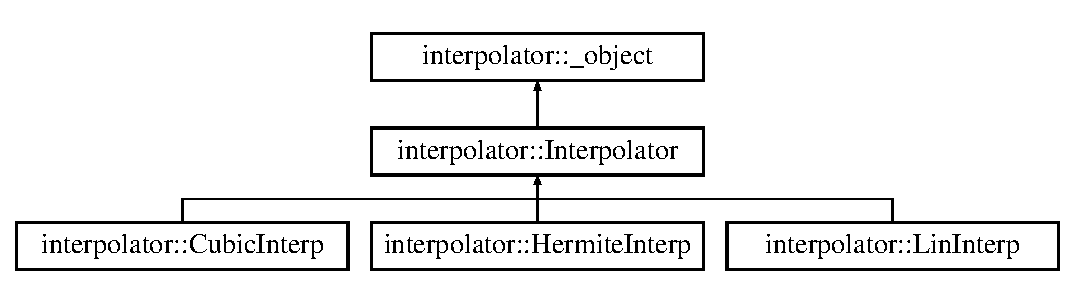
\includegraphics[height=3cm]{d9/d1b/classinterpolator_1_1__object}
\end{center}
\end{figure}


The documentation for this class was generated from the following file:\begin{DoxyCompactItemize}
\item 
src/interpolator.py\end{DoxyCompactItemize}

\hypertarget{classmatrix_1_1__object}{
\section{matrix::\_\-object Class Reference}
\label{d8/ddb/classmatrix_1_1__object}\index{matrix::\_\-object@{matrix::\_\-object}}
}
Inheritance diagram for matrix::\_\-object:\begin{figure}[H]
\begin{center}
\leavevmode
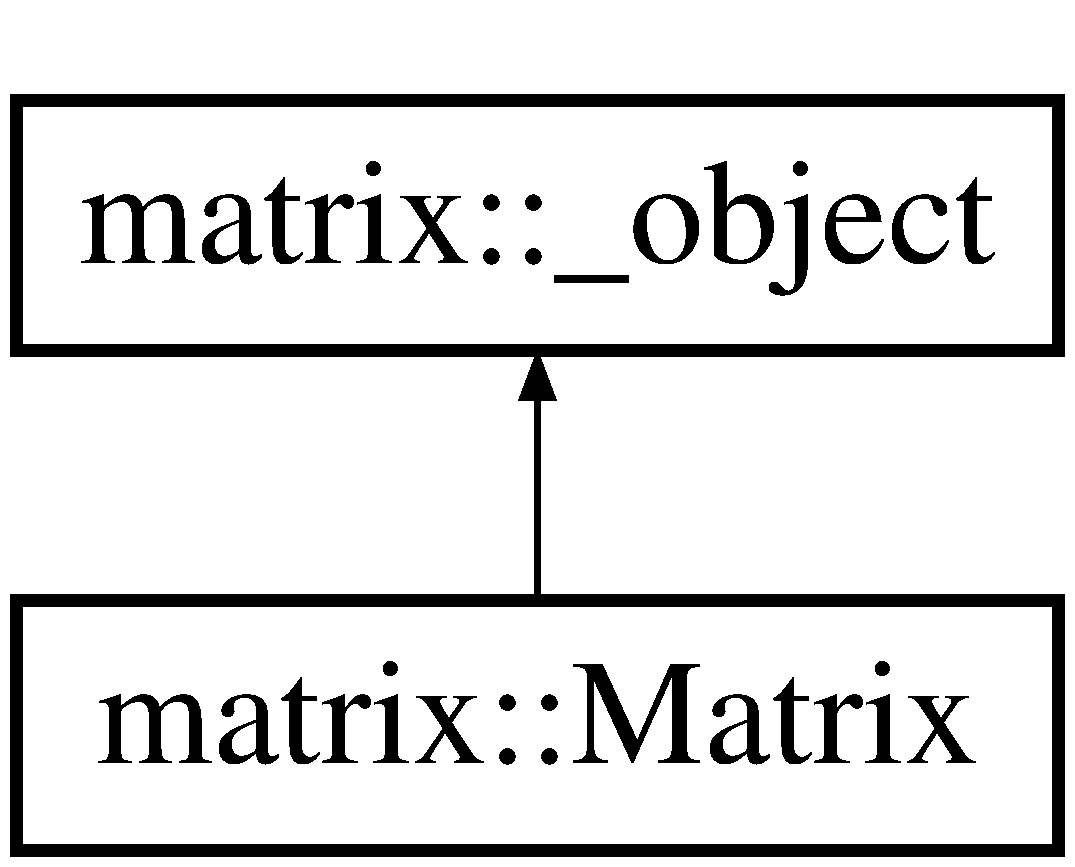
\includegraphics[height=2cm]{d8/ddb/classmatrix_1_1__object}
\end{center}
\end{figure}


The documentation for this class was generated from the following file:\begin{DoxyCompactItemize}
\item 
src/matrix.py\end{DoxyCompactItemize}

\hypertarget{classmatrix3d_1_1__object}{
\section{matrix3d::\_\-object Class Reference}
\label{d7/d99/classmatrix3d_1_1__object}\index{matrix3d::\_\-object@{matrix3d::\_\-object}}
}
Inheritance diagram for matrix3d::\_\-object:\begin{figure}[H]
\begin{center}
\leavevmode
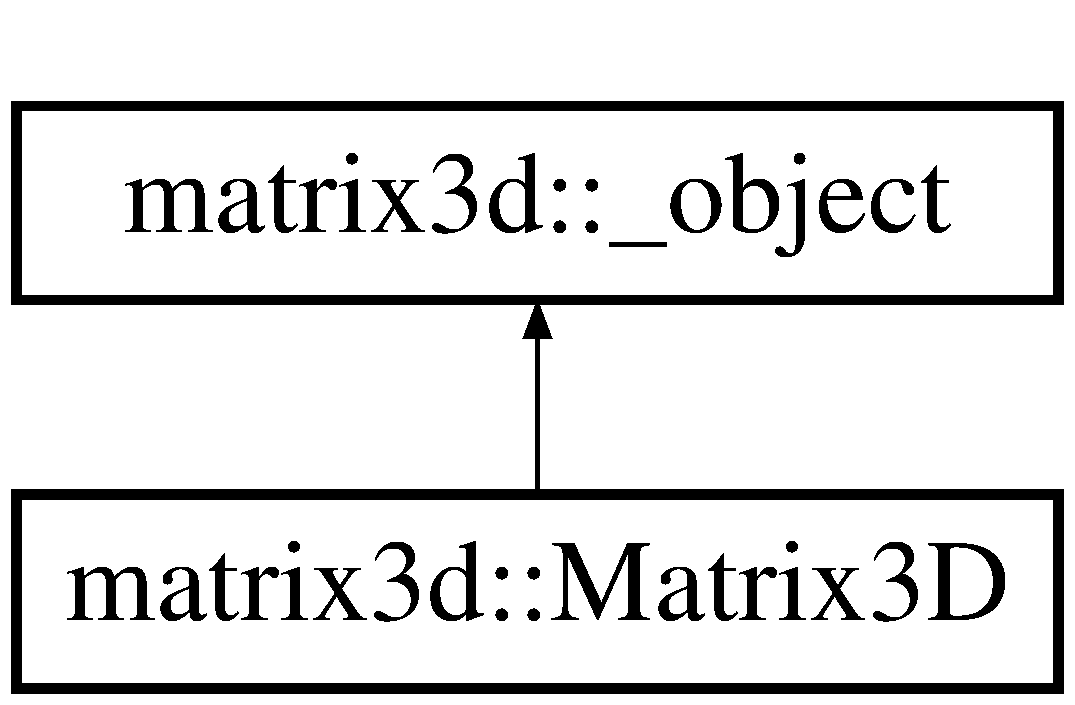
\includegraphics[height=2cm]{d7/d99/classmatrix3d_1_1__object}
\end{center}
\end{figure}


The documentation for this class was generated from the following file:\begin{DoxyCompactItemize}
\item 
src/matrix3d.py\end{DoxyCompactItemize}

\hypertarget{classmatrix4d_1_1__object}{
\section{matrix4d::\_\-object Class Reference}
\label{d5/df5/classmatrix4d_1_1__object}\index{matrix4d::\_\-object@{matrix4d::\_\-object}}
}
Inheritance diagram for matrix4d::\_\-object:\begin{figure}[H]
\begin{center}
\leavevmode
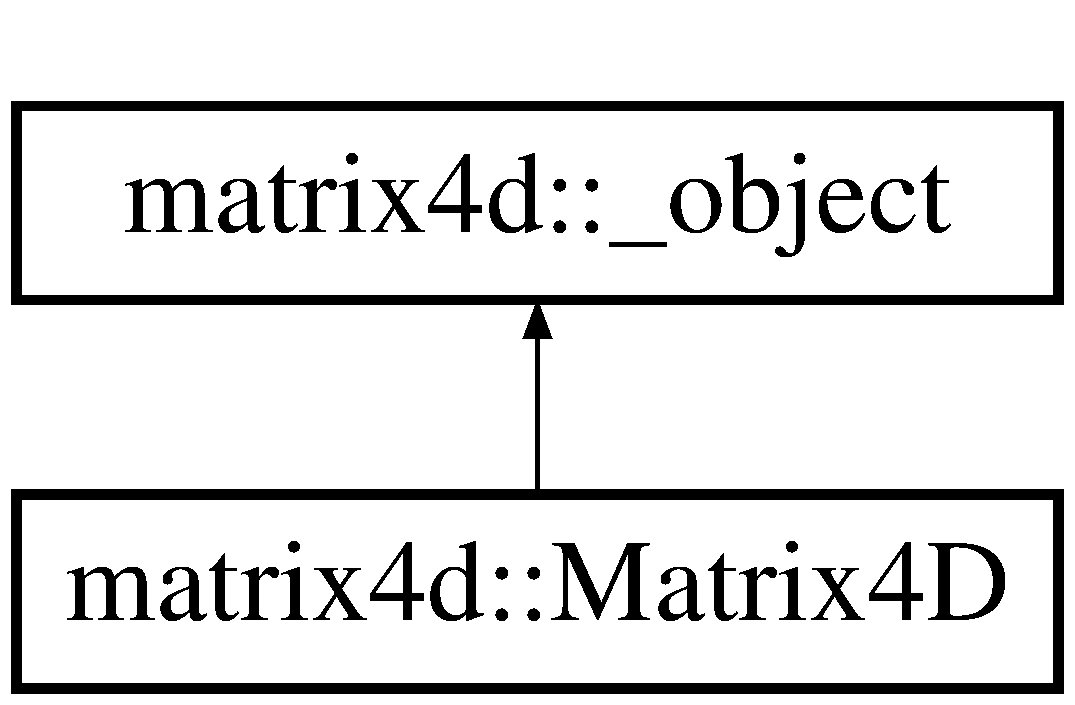
\includegraphics[height=2cm]{d5/df5/classmatrix4d_1_1__object}
\end{center}
\end{figure}


The documentation for this class was generated from the following file:\begin{DoxyCompactItemize}
\item 
src/matrix4d.py\end{DoxyCompactItemize}

\hypertarget{classmaxslope_1_1__object}{
\section{maxslope::\_\-object Class Reference}
\label{d1/d92/classmaxslope_1_1__object}\index{maxslope::\_\-object@{maxslope::\_\-object}}
}
Inheritance diagram for maxslope::\_\-object:\begin{figure}[H]
\begin{center}
\leavevmode
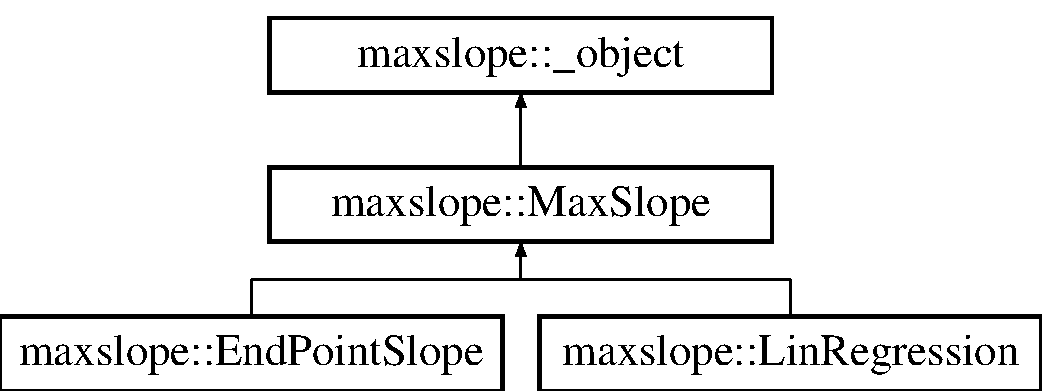
\includegraphics[height=3cm]{d1/d92/classmaxslope_1_1__object}
\end{center}
\end{figure}


The documentation for this class was generated from the following file:\begin{DoxyCompactItemize}
\item 
src/maxslope.py\end{DoxyCompactItemize}

\hypertarget{classmonocheck_1_1__object}{
\section{monocheck::\_\-object Class Reference}
\label{d8/dec/classmonocheck_1_1__object}\index{monocheck::\_\-object@{monocheck::\_\-object}}
}
Inheritance diagram for monocheck::\_\-object:\begin{figure}[H]
\begin{center}
\leavevmode
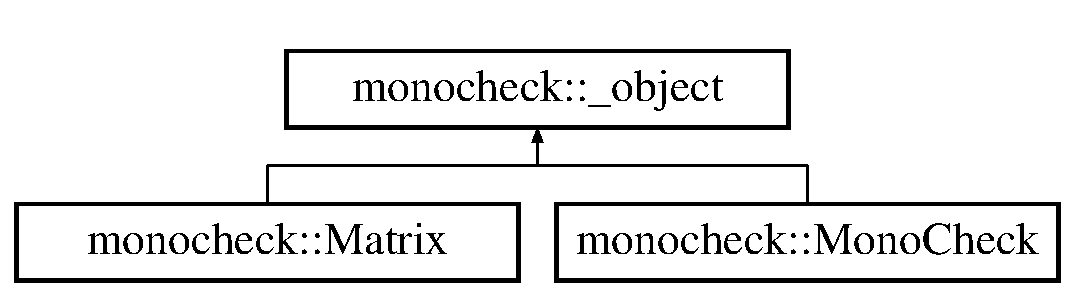
\includegraphics[height=2cm]{d8/dec/classmonocheck_1_1__object}
\end{center}
\end{figure}


The documentation for this class was generated from the following file:\begin{DoxyCompactItemize}
\item 
src/monocheck.py\end{DoxyCompactItemize}

\hypertarget{classintegrator_1_1__object}{
\section{integrator::\_\-object Class Reference}
\label{d6/d0c/classintegrator_1_1__object}\index{integrator::\_\-object@{integrator::\_\-object}}
}
Inheritance diagram for integrator::\_\-object:\begin{figure}[H]
\begin{center}
\leavevmode
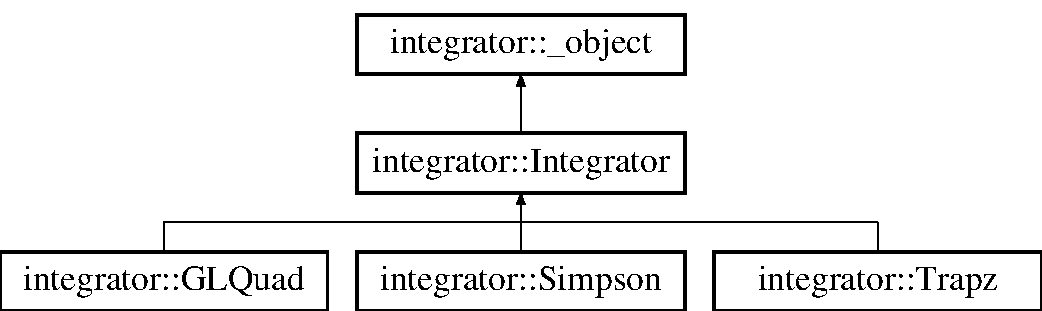
\includegraphics[height=3cm]{d6/d0c/classintegrator_1_1__object}
\end{center}
\end{figure}


The documentation for this class was generated from the following file:\begin{DoxyCompactItemize}
\item 
src/integrator.py\end{DoxyCompactItemize}

\hypertarget{classleastnonmono_1_1__object}{
\section{leastnonmono::\_\-object Class Reference}
\label{d0/dee/classleastnonmono_1_1__object}\index{leastnonmono::\_\-object@{leastnonmono::\_\-object}}
}
Inheritance diagram for leastnonmono::\_\-object:\begin{figure}[H]
\begin{center}
\leavevmode
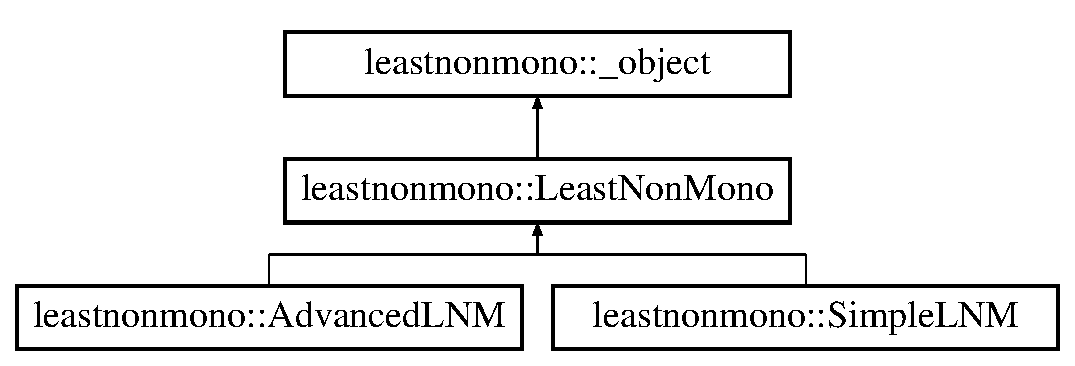
\includegraphics[height=3cm]{d0/dee/classleastnonmono_1_1__object}
\end{center}
\end{figure}


The documentation for this class was generated from the following file:\begin{DoxyCompactItemize}
\item 
src/leastnonmono.py\end{DoxyCompactItemize}

\hypertarget{classpdf_1_1__object}{
\section{pdf::\_\-object Class Reference}
\label{df/d35/classpdf_1_1__object}\index{pdf::\_\-object@{pdf::\_\-object}}
}
Inheritance diagram for pdf::\_\-object:\begin{figure}[H]
\begin{center}
\leavevmode
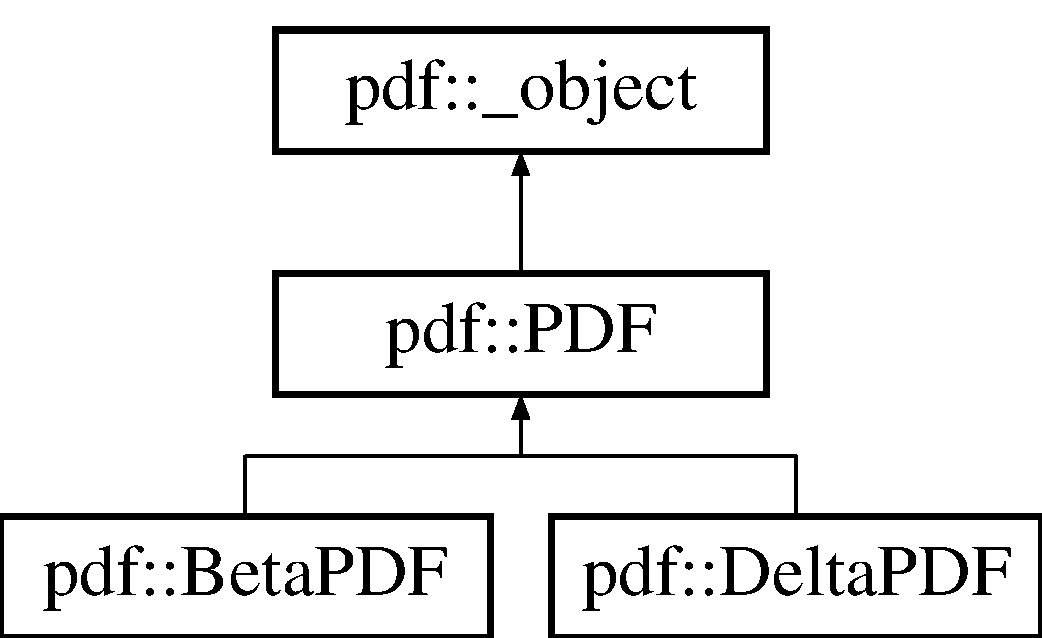
\includegraphics[height=3cm]{df/d35/classpdf_1_1__object}
\end{center}
\end{figure}


The documentation for this class was generated from the following file:\begin{DoxyCompactItemize}
\item 
src/pdf.py\end{DoxyCompactItemize}

\hypertarget{classsorting_1_1__object}{
\section{sorting::\_\-object Class Reference}
\label{da/d16/classsorting_1_1__object}\index{sorting::\_\-object@{sorting::\_\-object}}
}
Inheritance diagram for sorting::\_\-object:\begin{figure}[H]
\begin{center}
\leavevmode
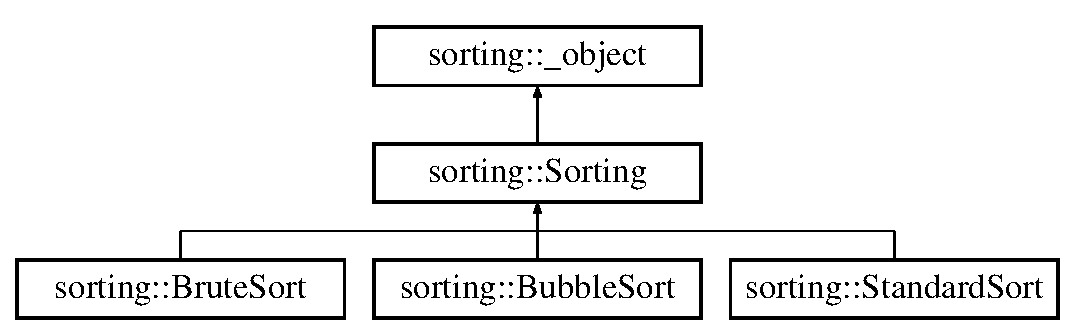
\includegraphics[height=3cm]{da/d16/classsorting_1_1__object}
\end{center}
\end{figure}


The documentation for this class was generated from the following file:\begin{DoxyCompactItemize}
\item 
src/sorting.py\end{DoxyCompactItemize}

\hypertarget{classAdvancedLNM}{
\section{AdvancedLNM Class Reference}
\label{dd/d1d/classAdvancedLNM}\index{AdvancedLNM@{AdvancedLNM}}
}
Inheritance diagram for AdvancedLNM:\begin{figure}[H]
\begin{center}
\leavevmode
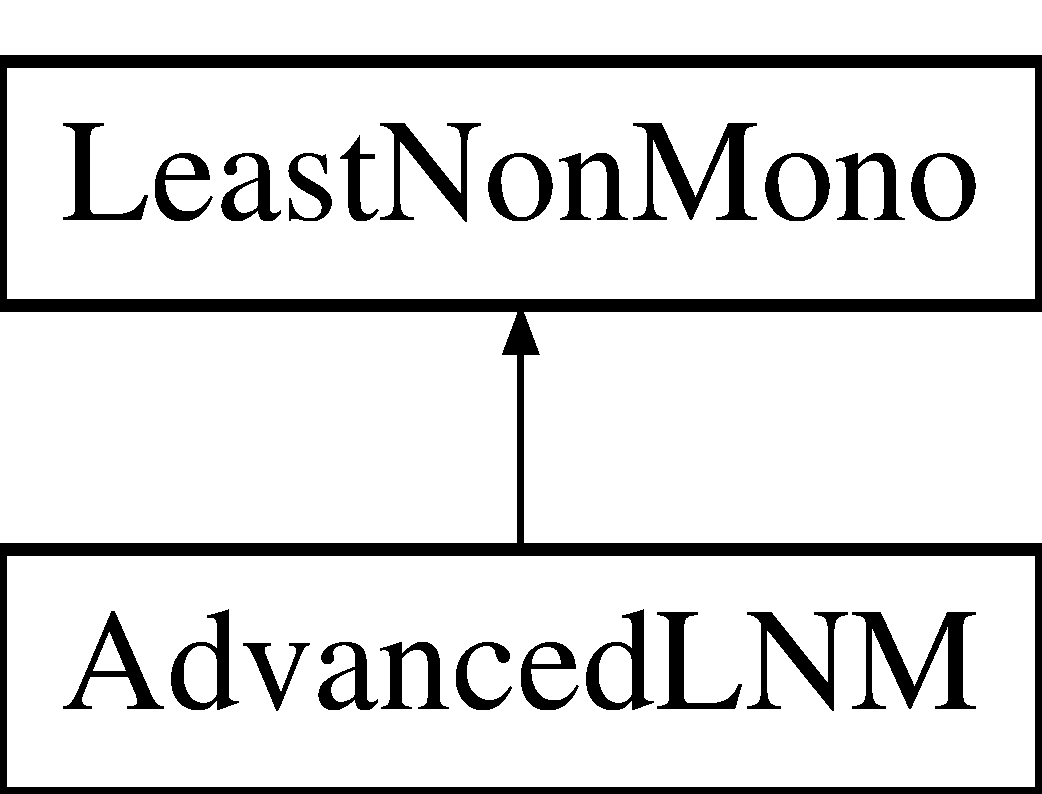
\includegraphics[height=2cm]{dd/d1d/classAdvancedLNM}
\end{center}
\end{figure}
\subsection*{Public Member Functions}
\begin{DoxyCompactItemize}
\item 
\hyperlink{classAdvancedLNM_af9317f34be7610889b8d37c606165ec4}{AdvancedLNM} (const \hyperlink{classMatrix}{Matrix} \&progVar)
\begin{DoxyCompactList}\small\item\em Constructor. \item\end{DoxyCompactList}\item 
\hypertarget{classAdvancedLNM_af44785dd7ff58621804d9911be88836a}{
\hyperlink{classAdvancedLNM_af44785dd7ff58621804d9911be88836a}{$\sim$AdvancedLNM} ()}
\label{dd/d1d/classAdvancedLNM_af44785dd7ff58621804d9911be88836a}

\begin{DoxyCompactList}\small\item\em Destructor. \item\end{DoxyCompactList}\item 
int \hyperlink{classAdvancedLNM_aaf028bdf53b6428371d122eb4cf343b4}{LeastNonMonotonic} (int $\ast$monoAry, const int ncols, const int col)
\begin{DoxyCompactList}\small\item\em Method to find least monotonic progress variable. \item\end{DoxyCompactList}\end{DoxyCompactItemize}


\subsection{Constructor \& Destructor Documentation}
\hypertarget{classAdvancedLNM_af9317f34be7610889b8d37c606165ec4}{
\index{AdvancedLNM@{AdvancedLNM}!AdvancedLNM@{AdvancedLNM}}
\index{AdvancedLNM@{AdvancedLNM}!AdvancedLNM@{AdvancedLNM}}
\subsubsection[{AdvancedLNM}]{\setlength{\rightskip}{0pt plus 5cm}AdvancedLNM::AdvancedLNM (const {\bf Matrix} \& {\em progVar})}}
\label{dd/d1d/classAdvancedLNM_af9317f34be7610889b8d37c606165ec4}


Constructor. 

\hyperlink{classAdvancedLNM}{AdvancedLNM} is a class that determines the least non-\/monotonic progress variable with respect to temperature (or another specified column). It determines the progress variable with the smallest percentage of non-\/unique (one-\/to-\/one) points and selects it as the least non-\/monotonic progress variable.

If two or more progress variables share the smallest percentage, then the progress variable with the greatest magnitude slope (by endpoints) is selected. 

\subsection{Member Function Documentation}
\hypertarget{classAdvancedLNM_aaf028bdf53b6428371d122eb4cf343b4}{
\index{AdvancedLNM@{AdvancedLNM}!LeastNonMonotonic@{LeastNonMonotonic}}
\index{LeastNonMonotonic@{LeastNonMonotonic}!AdvancedLNM@{AdvancedLNM}}
\subsubsection[{LeastNonMonotonic}]{\setlength{\rightskip}{0pt plus 5cm}int AdvancedLNM::LeastNonMonotonic (int $\ast$ {\em monoAry}, \/  const int {\em ncols}, \/  const int {\em col})\hspace{0.3cm}{\ttfamily  \mbox{[}virtual\mbox{]}}}}
\label{dd/d1d/classAdvancedLNM_aaf028bdf53b6428371d122eb4cf343b4}


Method to find least monotonic progress variable. 

LeastNonMonotonic calculates the percentage of non-\/unique points. The input array monoAry will initially be filled with 0s since all progress variables are non-\/monotonic. This method will select the least non-\/monotonic and change its value in monoAry to 1. col is the reference column.

\begin{DoxyVerb}
INPUTS:

int *monoAry     array containing integer flags that denote the monotonicity of candidate progress variables

const int ncols  number of columns of monoAry

const int col    the reference column 

OUTPUT:

int              flag specifying whether or not the function succeeded
                  = 0: success
		 != 0: something went wrong


\end{DoxyVerb}
 

Implements \hyperlink{classLeastNonMono_a239cbd7836950dc7c758138c4db00d0c}{LeastNonMono}.



The documentation for this class was generated from the following files:\begin{DoxyCompactItemize}
\item 
src/advancedlnm.h\item 
src/advancedlnm.cc\end{DoxyCompactItemize}

\hypertarget{classleastnonmono_1_1AdvancedLNM}{
\section{leastnonmono::AdvancedLNM Class Reference}
\label{db/d0a/classleastnonmono_1_1AdvancedLNM}\index{leastnonmono::AdvancedLNM@{leastnonmono::AdvancedLNM}}
}
Inheritance diagram for leastnonmono::AdvancedLNM:\begin{figure}[H]
\begin{center}
\leavevmode
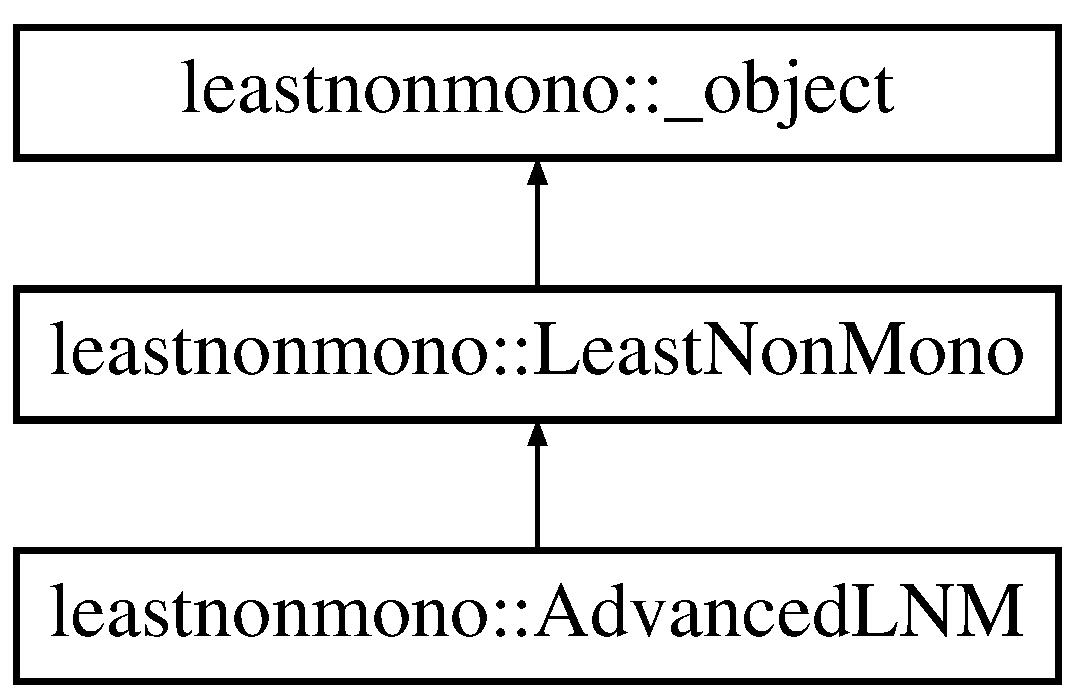
\includegraphics[height=3cm]{db/d0a/classleastnonmono_1_1AdvancedLNM}
\end{center}
\end{figure}
\subsection*{Public Member Functions}
\begin{DoxyCompactItemize}
\item 
\hypertarget{classleastnonmono_1_1AdvancedLNM_adc8d6450940ccc985c1e0925059ec082}{
def {\bfseries \_\-\_\-init\_\-\_\-}}
\label{db/d0a/classleastnonmono_1_1AdvancedLNM_adc8d6450940ccc985c1e0925059ec082}

\item 
\hypertarget{classleastnonmono_1_1AdvancedLNM_a8a6bd15664826960139bd89731fe9fa2}{
def {\bfseries LeastNonMonotonic}}
\label{db/d0a/classleastnonmono_1_1AdvancedLNM_a8a6bd15664826960139bd89731fe9fa2}

\end{DoxyCompactItemize}
\subsection*{Public Attributes}
\begin{DoxyCompactItemize}
\item 
\hypertarget{classleastnonmono_1_1AdvancedLNM_a7487bd57076caf8236ddd3733f776fdb}{
{\bfseries this}}
\label{db/d0a/classleastnonmono_1_1AdvancedLNM_a7487bd57076caf8236ddd3733f776fdb}

\end{DoxyCompactItemize}


The documentation for this class was generated from the following file:\begin{DoxyCompactItemize}
\item 
src/leastnonmono.py\end{DoxyCompactItemize}

\hypertarget{classBetaPDF}{
\section{BetaPDF Class Reference}
\label{de/d4f/classBetaPDF}\index{BetaPDF@{BetaPDF}}
}


Evaluates beta \hyperlink{classPDF}{PDF} and stores values in a \hyperlink{classMatrix3D}{Matrix3D} object.  




{\ttfamily \#include $<$betaPDF.h$>$}

Inheritance diagram for BetaPDF:\begin{figure}[H]
\begin{center}
\leavevmode
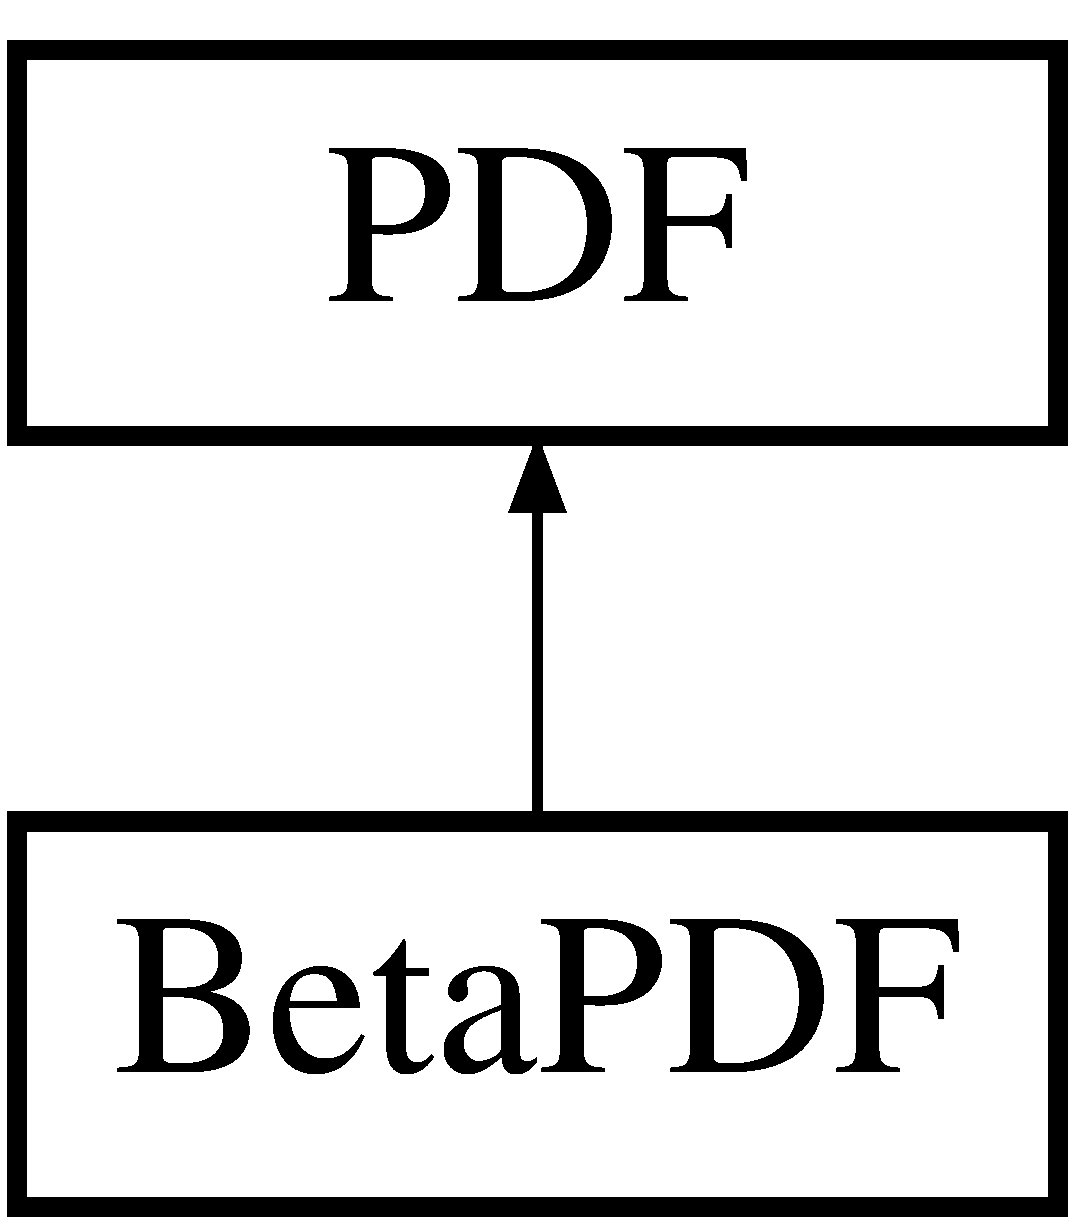
\includegraphics[height=2cm]{de/d4f/classBetaPDF}
\end{center}
\end{figure}
\subsection*{Public Member Functions}
\begin{DoxyCompactItemize}
\item 
\hypertarget{classBetaPDF_a0b5160ebefdcd8b696a45a131bab3261}{
\hyperlink{classBetaPDF_a0b5160ebefdcd8b696a45a131bab3261}{BetaPDF} (const double $\ast$Zmean, const int ZmeanPoints, const double $\ast$Zvar, const int ZvarPoints)}
\label{de/d4f/classBetaPDF_a0b5160ebefdcd8b696a45a131bab3261}

\begin{DoxyCompactList}\small\item\em Constructor. \item\end{DoxyCompactList}\item 
\hypertarget{classBetaPDF_a3394efd2861f7a2d5944365ea0edbe50}{
\hyperlink{classBetaPDF_a3394efd2861f7a2d5944365ea0edbe50}{$\sim$BetaPDF} ()}
\label{de/d4f/classBetaPDF_a3394efd2861f7a2d5944365ea0edbe50}

\begin{DoxyCompactList}\small\item\em Destructor. \item\end{DoxyCompactList}\item 
int \hyperlink{classBetaPDF_a5c27da056f9c9b17af0888fac7df2c9f}{pdfVal} (const double $\ast$Z, const int ZPoints, \hyperlink{classMatrix3D}{Matrix3D} $\ast$pdfValM)
\begin{DoxyCompactList}\small\item\em Main routine that generates the \hyperlink{classPDF}{PDF} values. \item\end{DoxyCompactList}\end{DoxyCompactItemize}


\subsection{Detailed Description}
Evaluates beta \hyperlink{classPDF}{PDF} and stores values in a \hyperlink{classMatrix3D}{Matrix3D} object. 

\subsection{Member Function Documentation}
\hypertarget{classBetaPDF_a5c27da056f9c9b17af0888fac7df2c9f}{
\index{BetaPDF@{BetaPDF}!pdfVal@{pdfVal}}
\index{pdfVal@{pdfVal}!BetaPDF@{BetaPDF}}
\subsubsection[{pdfVal}]{\setlength{\rightskip}{0pt plus 5cm}int BetaPDF::pdfVal (const double $\ast$ {\em Z}, \/  const int {\em ZPoints}, \/  {\bf Matrix3D} $\ast$ {\em pdfValM})\hspace{0.3cm}{\ttfamily  \mbox{[}virtual\mbox{]}}}}
\label{de/d4f/classBetaPDF_a5c27da056f9c9b17af0888fac7df2c9f}


Main routine that generates the \hyperlink{classPDF}{PDF} values. 

The Beta \hyperlink{classPDF}{PDF} uses statistics (means and variances) to generate a \hyperlink{classPDF}{PDF}. The \hyperlink{classPDF}{PDF} values are stored in a \hyperlink{classMatrix3D}{Matrix3D} object: dim1 is the variance, dim2 is the mean, and dim3 are the data points.

\begin{DoxyVerb}

  INPUTS: 
  const double* Z        double array containing mixture fraction values coming from the files

  const int ZPoints      number of mixture fraction values in the Z array

  Matrix3D* pdfValM      the Matrix3D type container that stores the PDF values

  
  OUTPUT:

  int                    flag specifying whether or not the function succeeded
                          = 0: success
			 != 0: something went wrong

  \end{DoxyVerb}
 

Implements \hyperlink{classPDF}{PDF}.



The documentation for this class was generated from the following files:\begin{DoxyCompactItemize}
\item 
src/betaPDF.h\item 
src/betaPDF.cc\end{DoxyCompactItemize}

\hypertarget{classpdf_1_1BetaPDF}{
\section{pdf::BetaPDF Class Reference}
\label{d4/dae/classpdf_1_1BetaPDF}\index{pdf::BetaPDF@{pdf::BetaPDF}}
}
Inheritance diagram for pdf::BetaPDF:\begin{figure}[H]
\begin{center}
\leavevmode
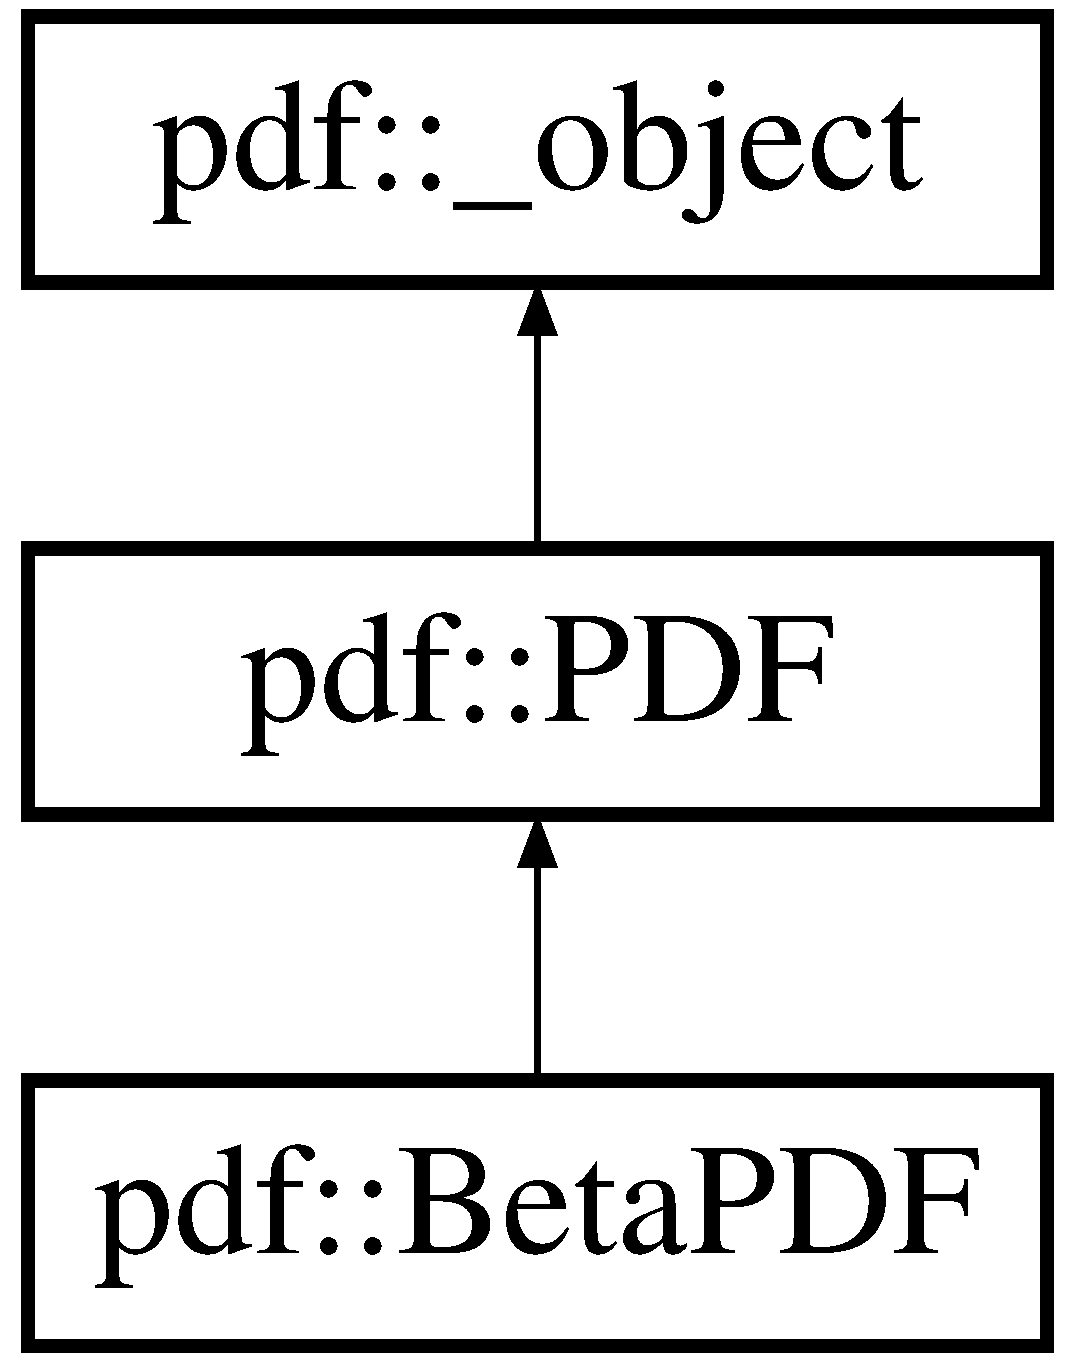
\includegraphics[height=3cm]{d4/dae/classpdf_1_1BetaPDF}
\end{center}
\end{figure}
\subsection*{Public Member Functions}
\begin{DoxyCompactItemize}
\item 
\hypertarget{classpdf_1_1BetaPDF_a20df6a985b59544305063ed17b7358c5}{
def {\bfseries \_\-\_\-init\_\-\_\-}}
\label{d4/dae/classpdf_1_1BetaPDF_a20df6a985b59544305063ed17b7358c5}

\item 
\hypertarget{classpdf_1_1BetaPDF_ad7f9b56263693e180c38d788048299f0}{
def {\bfseries pdfVal}}
\label{d4/dae/classpdf_1_1BetaPDF_ad7f9b56263693e180c38d788048299f0}

\end{DoxyCompactItemize}
\subsection*{Public Attributes}
\begin{DoxyCompactItemize}
\item 
\hypertarget{classpdf_1_1BetaPDF_afec5aec12f1405624850046968b2bbec}{
{\bfseries this}}
\label{d4/dae/classpdf_1_1BetaPDF_afec5aec12f1405624850046968b2bbec}

\end{DoxyCompactItemize}


The documentation for this class was generated from the following file:\begin{DoxyCompactItemize}
\item 
src/pdf.py\end{DoxyCompactItemize}

\hypertarget{classBruteSort}{
\section{BruteSort Class Reference}
\label{d7/d98/classBruteSort}\index{BruteSort@{BruteSort}}
}
Inheritance diagram for BruteSort:\begin{figure}[H]
\begin{center}
\leavevmode
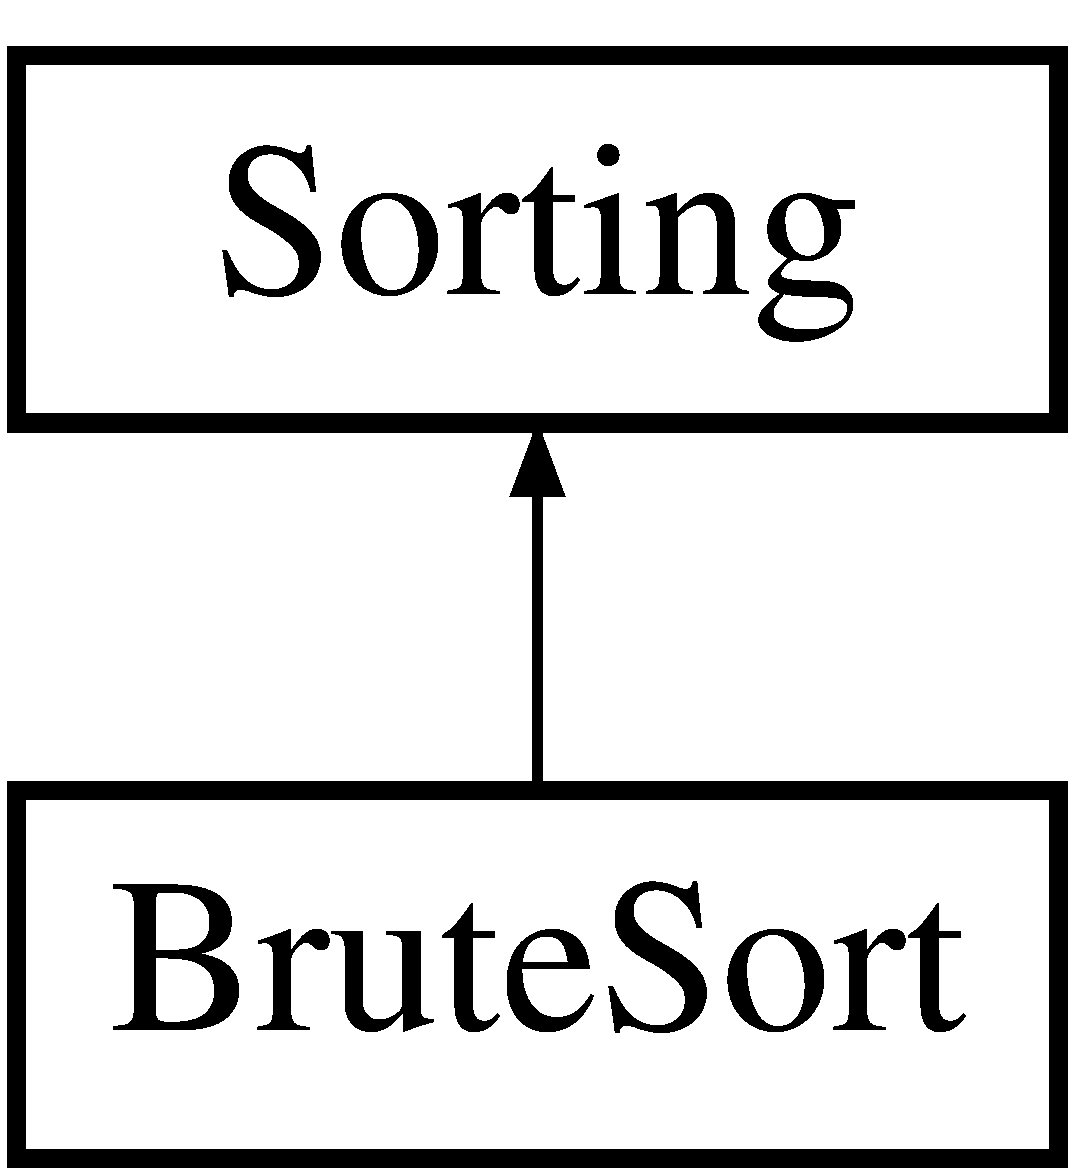
\includegraphics[height=2cm]{d7/d98/classBruteSort}
\end{center}
\end{figure}
\subsection*{Public Member Functions}
\begin{DoxyCompactItemize}
\item 
\hyperlink{classBruteSort_af173d86f16480c1e08de8cb156d29205}{BruteSort} (\hyperlink{classMatrix}{Matrix} $\ast$data)
\begin{DoxyCompactList}\small\item\em Constructor. \item\end{DoxyCompactList}\item 
\hypertarget{classBruteSort_a0bbf682f921452842e844599b1f02c0a}{
\hyperlink{classBruteSort_a0bbf682f921452842e844599b1f02c0a}{$\sim$BruteSort} ()}
\label{d7/d98/classBruteSort_a0bbf682f921452842e844599b1f02c0a}

\begin{DoxyCompactList}\small\item\em Destructor. \item\end{DoxyCompactList}\item 
int \hyperlink{classBruteSort_ae1345f8f8ddc289832816d900226fc1e}{sort\_\-data} ()
\begin{DoxyCompactList}\small\item\em Main function that sorts the given data. \item\end{DoxyCompactList}\item 
\hypertarget{classBruteSort_a7e765945892481b5ca40fd88ab5f1e6f}{
void \hyperlink{classBruteSort_a7e765945892481b5ca40fd88ab5f1e6f}{SetRefColNum} (int num)}
\label{d7/d98/classBruteSort_a7e765945892481b5ca40fd88ab5f1e6f}

\begin{DoxyCompactList}\small\item\em Set the reference column number. \item\end{DoxyCompactList}\end{DoxyCompactItemize}


\subsection{Constructor \& Destructor Documentation}
\hypertarget{classBruteSort_af173d86f16480c1e08de8cb156d29205}{
\index{BruteSort@{BruteSort}!BruteSort@{BruteSort}}
\index{BruteSort@{BruteSort}!BruteSort@{BruteSort}}
\subsubsection[{BruteSort}]{\setlength{\rightskip}{0pt plus 5cm}BruteSort::BruteSort ({\bf Matrix} $\ast$ {\em data})}}
\label{d7/d98/classBruteSort_af173d86f16480c1e08de8cb156d29205}


Constructor. 

This algorithm goes over the each entry (rows times) at the selected column, finds the maximum entry, records its index. This is repeated rows times until the indices of the entries are obtained in order. Then each column of the matrix is reordered using these indices. 

\subsection{Member Function Documentation}
\hypertarget{classBruteSort_ae1345f8f8ddc289832816d900226fc1e}{
\index{BruteSort@{BruteSort}!sort\_\-data@{sort\_\-data}}
\index{sort\_\-data@{sort\_\-data}!BruteSort@{BruteSort}}
\subsubsection[{sort\_\-data}]{\setlength{\rightskip}{0pt plus 5cm}int BruteSort::sort\_\-data ()\hspace{0.3cm}{\ttfamily  \mbox{[}virtual\mbox{]}}}}
\label{d7/d98/classBruteSort_ae1345f8f8ddc289832816d900226fc1e}


Main function that sorts the given data. 

The algortihm processes the reference column and sorts it using the brute sort approach.

\begin{DoxyVerb}
  INPUT:

  There are no inputs. The data to be sorted is already passed via the constructor

  
  OUTPUT:

  int          flag specifying whether or not the function succeeded
                = 0: success
	       != 0: something went wrong

  \end{DoxyVerb}
 

Implements \hyperlink{classSorting_a6686201265fbb31ba9c2071623742be1}{Sorting}.



The documentation for this class was generated from the following files:\begin{DoxyCompactItemize}
\item 
src/brutesort.h\item 
src/brutesort.cc\end{DoxyCompactItemize}

\hypertarget{classsorting_1_1BruteSort}{
\section{sorting::BruteSort Class Reference}
\label{d3/dc2/classsorting_1_1BruteSort}\index{sorting::BruteSort@{sorting::BruteSort}}
}
Inheritance diagram for sorting::BruteSort:\begin{figure}[H]
\begin{center}
\leavevmode
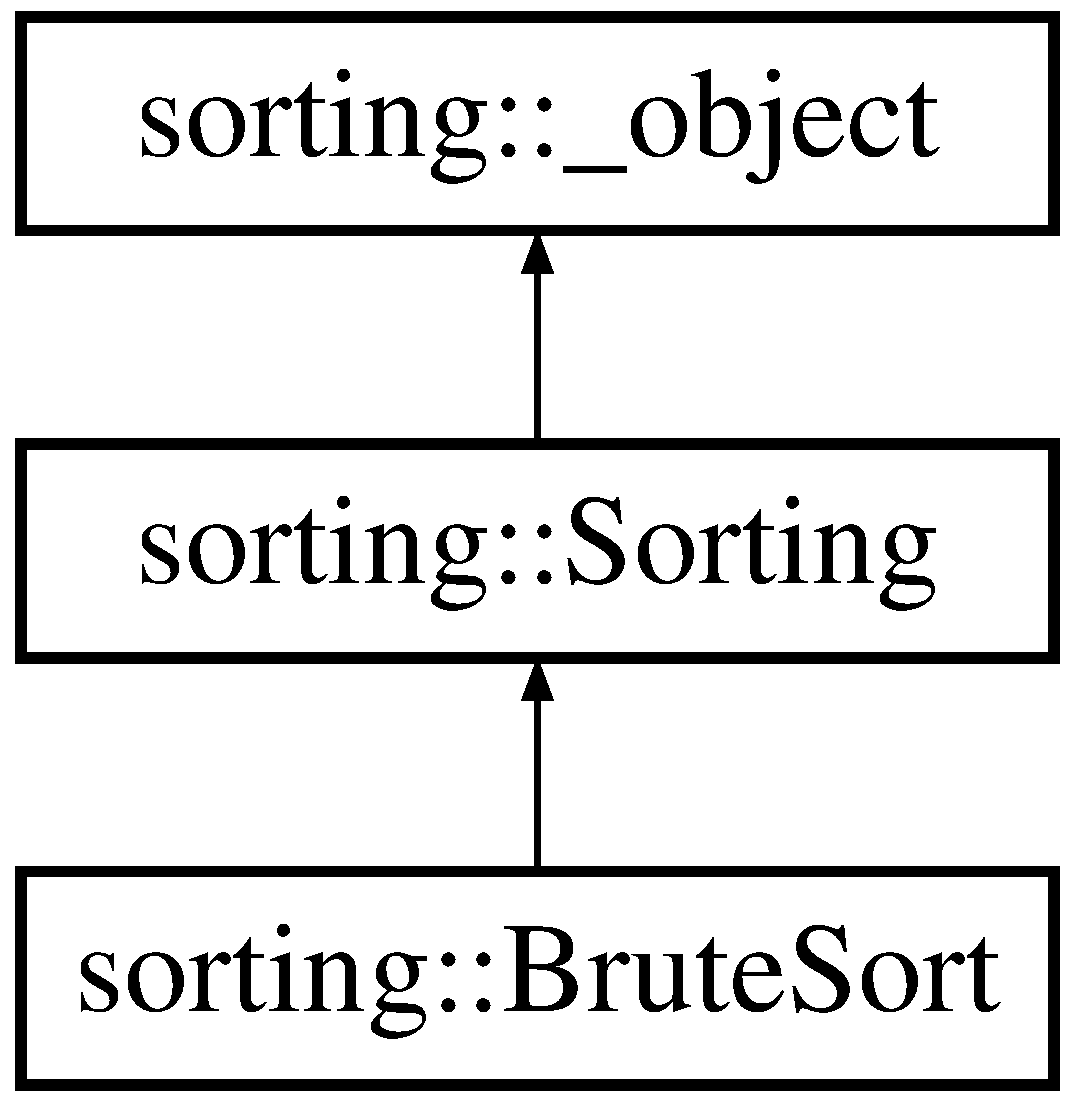
\includegraphics[height=3cm]{d3/dc2/classsorting_1_1BruteSort}
\end{center}
\end{figure}
\subsection*{Public Member Functions}
\begin{DoxyCompactItemize}
\item 
\hypertarget{classsorting_1_1BruteSort_ab23764289597790c5cdef1524bba8beb}{
def {\bfseries \_\-\_\-init\_\-\_\-}}
\label{d3/dc2/classsorting_1_1BruteSort_ab23764289597790c5cdef1524bba8beb}

\item 
\hypertarget{classsorting_1_1BruteSort_a02742dba963ab95c7f1f0106107b7234}{
def {\bfseries sort\_\-data}}
\label{d3/dc2/classsorting_1_1BruteSort_a02742dba963ab95c7f1f0106107b7234}

\item 
\hypertarget{classsorting_1_1BruteSort_a601fe10f0942c6fd6707eda68b7ec40a}{
def {\bfseries SetRefColNum}}
\label{d3/dc2/classsorting_1_1BruteSort_a601fe10f0942c6fd6707eda68b7ec40a}

\end{DoxyCompactItemize}
\subsection*{Public Attributes}
\begin{DoxyCompactItemize}
\item 
\hypertarget{classsorting_1_1BruteSort_abaf959081e7032ed48fe657be3d1c034}{
{\bfseries this}}
\label{d3/dc2/classsorting_1_1BruteSort_abaf959081e7032ed48fe657be3d1c034}

\end{DoxyCompactItemize}


The documentation for this class was generated from the following file:\begin{DoxyCompactItemize}
\item 
src/sorting.py\end{DoxyCompactItemize}

\hypertarget{classBubbleSort}{
\section{BubbleSort Class Reference}
\label{d9/d2a/classBubbleSort}\index{BubbleSort@{BubbleSort}}
}
Inheritance diagram for BubbleSort:\begin{figure}[H]
\begin{center}
\leavevmode
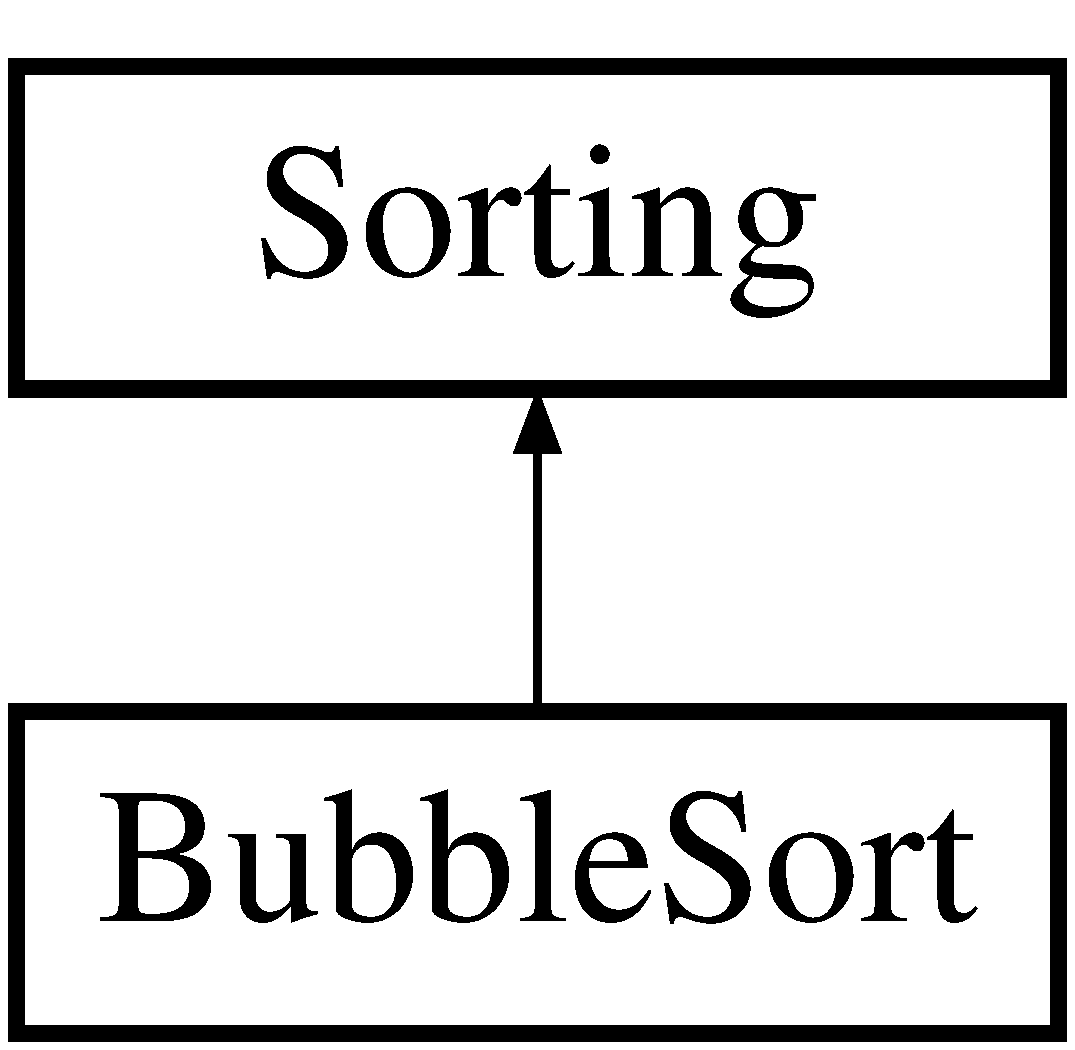
\includegraphics[height=2cm]{d9/d2a/classBubbleSort}
\end{center}
\end{figure}
\subsection*{Public Member Functions}
\begin{DoxyCompactItemize}
\item 
\hyperlink{classBubbleSort_a73599d7344bec5da6fb773c598500a60}{BubbleSort} (\hyperlink{classMatrix}{Matrix} $\ast$data)
\item 
\hypertarget{classBubbleSort_ac04244c2a98e23b093a24ffda60ae48a}{
\hyperlink{classBubbleSort_ac04244c2a98e23b093a24ffda60ae48a}{$\sim$BubbleSort} ()}
\label{d9/d2a/classBubbleSort_ac04244c2a98e23b093a24ffda60ae48a}

\begin{DoxyCompactList}\small\item\em Destructor. \item\end{DoxyCompactList}\item 
int \hyperlink{classBubbleSort_adec94eefc1117e7f302b303f5268c53a}{sort\_\-data} ()
\begin{DoxyCompactList}\small\item\em Main sorting body. \item\end{DoxyCompactList}\item 
\hypertarget{classBubbleSort_a6e78d7424bd49c3d1586d57e7b137756}{
void \hyperlink{classBubbleSort_a6e78d7424bd49c3d1586d57e7b137756}{SetRefColNum} (int num)}
\label{d9/d2a/classBubbleSort_a6e78d7424bd49c3d1586d57e7b137756}

\begin{DoxyCompactList}\small\item\em Set the reference column number and extract the data of the reference column to the container refColumn\_\-. \item\end{DoxyCompactList}\end{DoxyCompactItemize}


\subsection{Constructor \& Destructor Documentation}
\hypertarget{classBubbleSort_a73599d7344bec5da6fb773c598500a60}{
\index{BubbleSort@{BubbleSort}!BubbleSort@{BubbleSort}}
\index{BubbleSort@{BubbleSort}!BubbleSort@{BubbleSort}}
\subsubsection[{BubbleSort}]{\setlength{\rightskip}{0pt plus 5cm}BubbleSort::BubbleSort ({\bf Matrix} $\ast$ {\em data})}}
\label{d9/d2a/classBubbleSort_a73599d7344bec5da6fb773c598500a60}
The constructor duplicates the data from the matrix pointer to datacopy\_\- object. It also generates the array containing the indices to be used during sorting. 

\subsection{Member Function Documentation}
\hypertarget{classBubbleSort_adec94eefc1117e7f302b303f5268c53a}{
\index{BubbleSort@{BubbleSort}!sort\_\-data@{sort\_\-data}}
\index{sort\_\-data@{sort\_\-data}!BubbleSort@{BubbleSort}}
\subsubsection[{sort\_\-data}]{\setlength{\rightskip}{0pt plus 5cm}int BubbleSort::sort\_\-data ()\hspace{0.3cm}{\ttfamily  \mbox{[}virtual\mbox{]}}}}
\label{d9/d2a/classBubbleSort_adec94eefc1117e7f302b303f5268c53a}


Main sorting body. 

This function processes the reference column with the bubble sorting algorithm.

Details of the bubble sort algortihm can be found from the following link: \href{http://en.wikipedia.org/wiki/Bubble_sort}{\tt http://en.wikipedia.org/wiki/Bubble\_\-sort}

\begin{DoxyVerb}
  INPUT

  There are no inputs. The data to be sorted is already passed via the constructor

  OUTPUT:

  int         flag specifying whether or not the function succeeded
               = 0: success
	      != 0: something went wrong

  \end{DoxyVerb}
 

Implements \hyperlink{classSorting_a6686201265fbb31ba9c2071623742be1}{Sorting}.



The documentation for this class was generated from the following files:\begin{DoxyCompactItemize}
\item 
src/bubblesort.h\item 
src/bubblesort.cc\end{DoxyCompactItemize}

\hypertarget{classsorting_1_1BubbleSort}{
\section{sorting::BubbleSort Class Reference}
\label{d2/df3/classsorting_1_1BubbleSort}\index{sorting::BubbleSort@{sorting::BubbleSort}}
}
Inheritance diagram for sorting::BubbleSort:\begin{figure}[H]
\begin{center}
\leavevmode
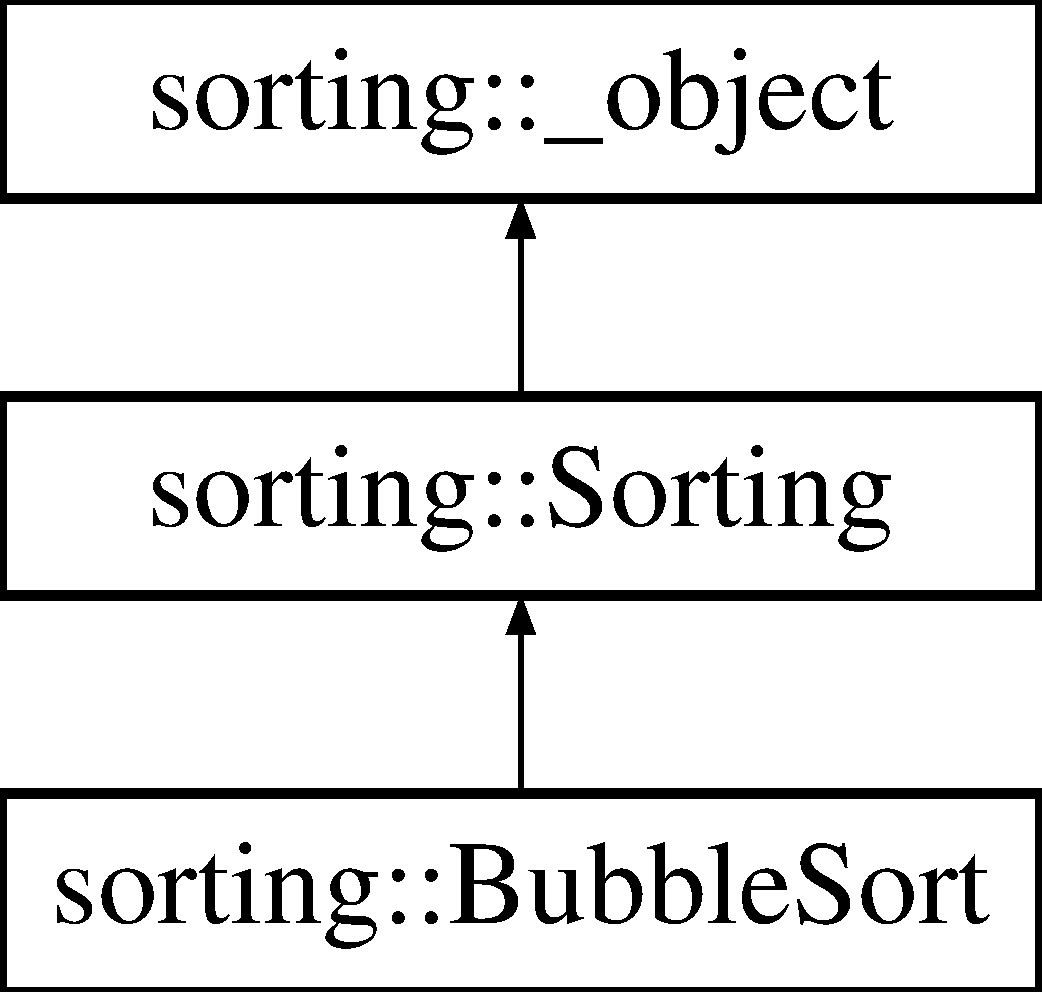
\includegraphics[height=3cm]{d2/df3/classsorting_1_1BubbleSort}
\end{center}
\end{figure}
\subsection*{Public Member Functions}
\begin{DoxyCompactItemize}
\item 
\hypertarget{classsorting_1_1BubbleSort_a085714342ebc22e2621a9c2764b4fffc}{
def {\bfseries \_\-\_\-init\_\-\_\-}}
\label{d2/df3/classsorting_1_1BubbleSort_a085714342ebc22e2621a9c2764b4fffc}

\item 
\hypertarget{classsorting_1_1BubbleSort_a5ecb956b8a3c882303b00f0fca833f8e}{
def {\bfseries sort\_\-data}}
\label{d2/df3/classsorting_1_1BubbleSort_a5ecb956b8a3c882303b00f0fca833f8e}

\item 
\hypertarget{classsorting_1_1BubbleSort_ae2a1b854b9d4be168e5c16853e1158b6}{
def {\bfseries SetRefColNum}}
\label{d2/df3/classsorting_1_1BubbleSort_ae2a1b854b9d4be168e5c16853e1158b6}

\end{DoxyCompactItemize}
\subsection*{Public Attributes}
\begin{DoxyCompactItemize}
\item 
\hypertarget{classsorting_1_1BubbleSort_aad1e6f3f63d7717a890f426cc024d42d}{
{\bfseries this}}
\label{d2/df3/classsorting_1_1BubbleSort_aad1e6f3f63d7717a890f426cc024d42d}

\end{DoxyCompactItemize}


The documentation for this class was generated from the following file:\begin{DoxyCompactItemize}
\item 
src/sorting.py\end{DoxyCompactItemize}

\hypertarget{classCompVec}{
\section{CompVec Class Reference}
\label{d7/d1f/classCompVec}\index{CompVec@{CompVec}}
}


Comparator for the standard sorting algorithm.  


\subsection*{Public Member Functions}
\begin{DoxyCompactItemize}
\item 
\hypertarget{classCompVec_a6963b86bb7b027c564f9fcbfa48631ff}{
{\bfseries CompVec} (double $\ast$arr)}
\label{d7/d1f/classCompVec_a6963b86bb7b027c564f9fcbfa48631ff}

\item 
\hypertarget{classCompVec_af72aba58e4ec029df30580c71c965490}{
bool {\bfseries operator()} (size\_\-t i, size\_\-t j)}
\label{d7/d1f/classCompVec_af72aba58e4ec029df30580c71c965490}

\end{DoxyCompactItemize}


\subsection{Detailed Description}
Comparator for the standard sorting algorithm. 

The documentation for this class was generated from the following file:\begin{DoxyCompactItemize}
\item 
src/standardsort.cc\end{DoxyCompactItemize}

\hypertarget{classinterpolator_1_1CubicInterp}{
\section{interpolator::CubicInterp Class Reference}
\label{d6/dab/classinterpolator_1_1CubicInterp}\index{interpolator::CubicInterp@{interpolator::CubicInterp}}
}
Inheritance diagram for interpolator::CubicInterp:\begin{figure}[H]
\begin{center}
\leavevmode
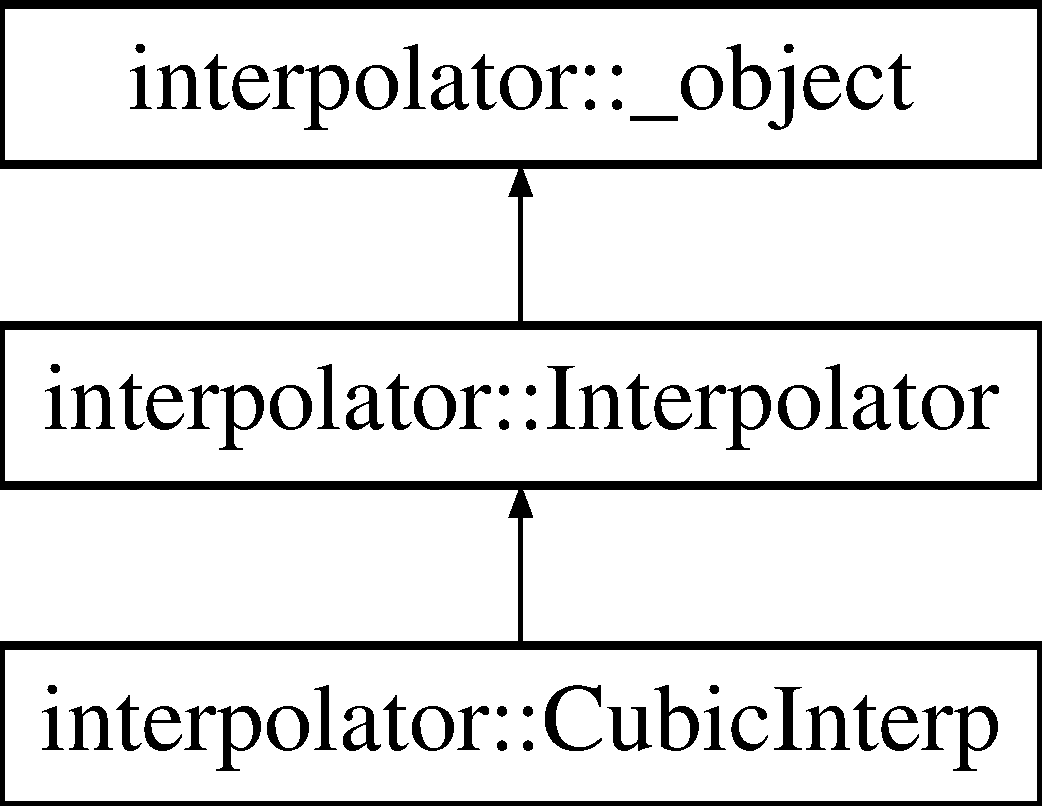
\includegraphics[height=3cm]{d6/dab/classinterpolator_1_1CubicInterp}
\end{center}
\end{figure}
\subsection*{Public Member Functions}
\begin{DoxyCompactItemize}
\item 
\hypertarget{classinterpolator_1_1CubicInterp_a8459c3cc860867050307b5c585c66c17}{
def {\bfseries \_\-\_\-init\_\-\_\-}}
\label{d6/dab/classinterpolator_1_1CubicInterp_a8459c3cc860867050307b5c585c66c17}

\item 
\hypertarget{classinterpolator_1_1CubicInterp_a687acfea9e0e656291277a79efda8a01}{
def {\bfseries Interp}}
\label{d6/dab/classinterpolator_1_1CubicInterp_a687acfea9e0e656291277a79efda8a01}

\end{DoxyCompactItemize}
\subsection*{Public Attributes}
\begin{DoxyCompactItemize}
\item 
\hypertarget{classinterpolator_1_1CubicInterp_a6929d792f1361b0c3e60a68814773b12}{
{\bfseries this}}
\label{d6/dab/classinterpolator_1_1CubicInterp_a6929d792f1361b0c3e60a68814773b12}

\end{DoxyCompactItemize}


The documentation for this class was generated from the following file:\begin{DoxyCompactItemize}
\item 
src/interpolator.py\end{DoxyCompactItemize}

\hypertarget{classCubicInterp}{
\section{CubicInterp Class Reference}
\label{dd/de9/classCubicInterp}\index{CubicInterp@{CubicInterp}}
}
Inheritance diagram for CubicInterp:\begin{figure}[H]
\begin{center}
\leavevmode
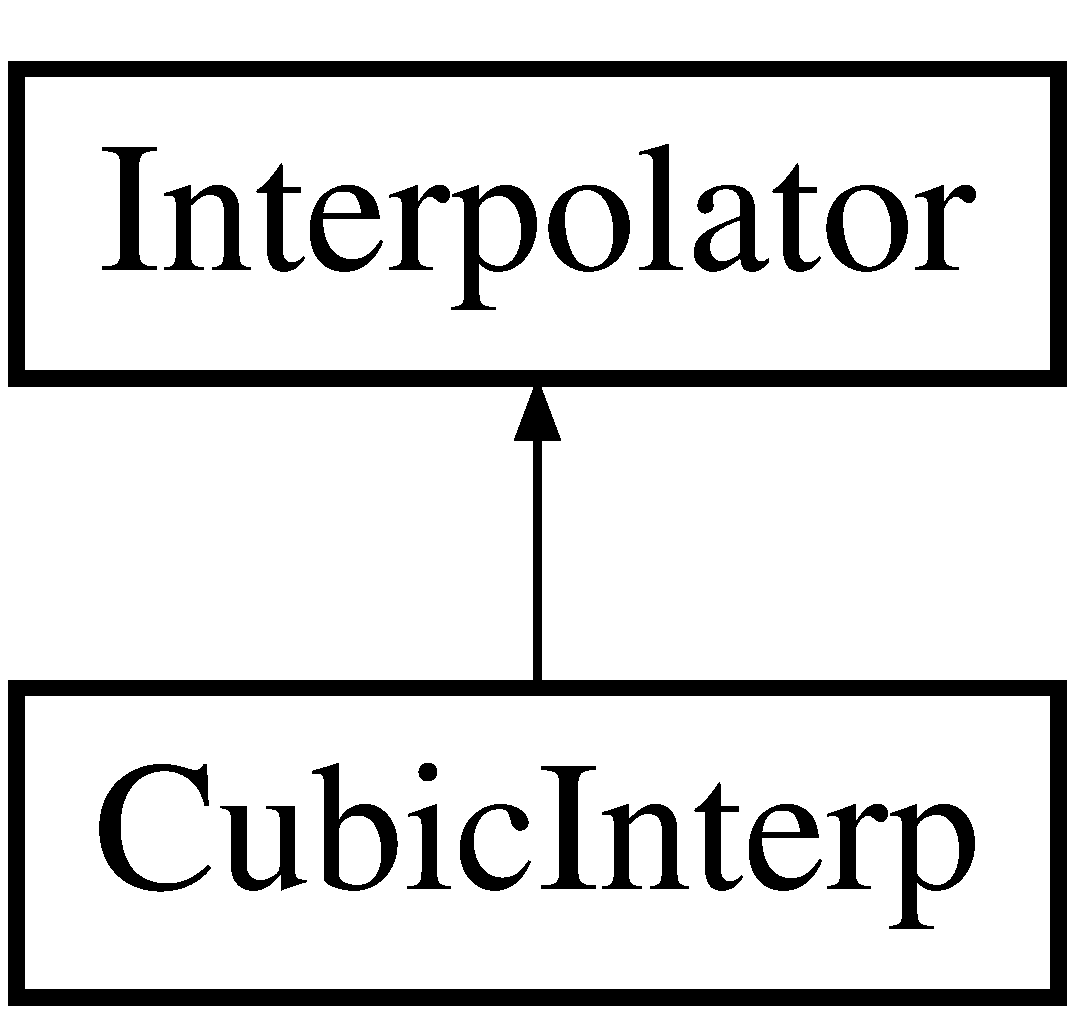
\includegraphics[height=2cm]{dd/de9/classCubicInterp}
\end{center}
\end{figure}
\subsection*{Public Member Functions}
\begin{DoxyCompactItemize}
\item 
\hypertarget{classCubicInterp_a4eb9093b962cbe527df14938016ea1a6}{
\hyperlink{classCubicInterp_a4eb9093b962cbe527df14938016ea1a6}{CubicInterp} ()}
\label{dd/de9/classCubicInterp_a4eb9093b962cbe527df14938016ea1a6}

\begin{DoxyCompactList}\small\item\em Constructor. \item\end{DoxyCompactList}\item 
\hypertarget{classCubicInterp_a57dd187897a0729518521a76c9f22818}{
\hyperlink{classCubicInterp_a57dd187897a0729518521a76c9f22818}{$\sim$CubicInterp} ()}
\label{dd/de9/classCubicInterp_a57dd187897a0729518521a76c9f22818}

\begin{DoxyCompactList}\small\item\em Destructor. \item\end{DoxyCompactList}\item 
int \hyperlink{classCubicInterp_a19da3e57e56c37f0b83f37f7217a8a0c}{Interp} (const \hyperlink{classMatrix}{Matrix} $\ast$matin, int col, double ival, double $\ast$vecout, int cols)
\begin{DoxyCompactList}\small\item\em Cubic spline interpolation function. \item\end{DoxyCompactList}\end{DoxyCompactItemize}


\subsection{Member Function Documentation}
\hypertarget{classCubicInterp_a19da3e57e56c37f0b83f37f7217a8a0c}{
\index{CubicInterp@{CubicInterp}!Interp@{Interp}}
\index{Interp@{Interp}!CubicInterp@{CubicInterp}}
\subsubsection[{Interp}]{\setlength{\rightskip}{0pt plus 5cm}int CubicInterp::Interp (const {\bf Matrix} $\ast$ {\em matin}, \/  int {\em col}, \/  double {\em ival}, \/  double $\ast$ {\em vecout}, \/  int {\em cols})\hspace{0.3cm}{\ttfamily  \mbox{[}virtual\mbox{]}}}}
\label{dd/de9/classCubicInterp_a19da3e57e56c37f0b83f37f7217a8a0c}


Cubic spline interpolation function. 

This function takes in a 2D matrix of data and interpolates an entire row from it using a cubic spline interpolator. Each column of the matrix is treated as a variable, with a specified column being the independent variable. The input data is assumed to be sorted by the independent variable.

\begin{DoxyVerb}
  INPUTS:

  const Matrix *matin    pointer to a Matrix object. This is the input data.

  int col                integer specifying which column of the input Matrix is the independent
                         variable

  double ival            value at which to interpolate

  double *vecout         pointer to an array which contains the interpolated row. This array has
                         the same number of columns as the input Matrix.

  int cols               number of columns of matin/vecout

  OUTPUTS:

  int                    flag specifying whether or not the function succeeded
                         = 0: success
			 = 1: extrapolation attempted
  \end{DoxyVerb}
 

Implements \hyperlink{classInterpolator_a2238defccb009047f624bda33cc47c73}{Interpolator}.



The documentation for this class was generated from the following files:\begin{DoxyCompactItemize}
\item 
src/cubicinterp.h\item 
src/cubicinterp.cc\end{DoxyCompactItemize}

\hypertarget{classpdf_1_1DeltaPDF}{
\section{pdf::DeltaPDF Class Reference}
\label{dc/d18/classpdf_1_1DeltaPDF}\index{pdf::DeltaPDF@{pdf::DeltaPDF}}
}
Inheritance diagram for pdf::DeltaPDF:\begin{figure}[H]
\begin{center}
\leavevmode
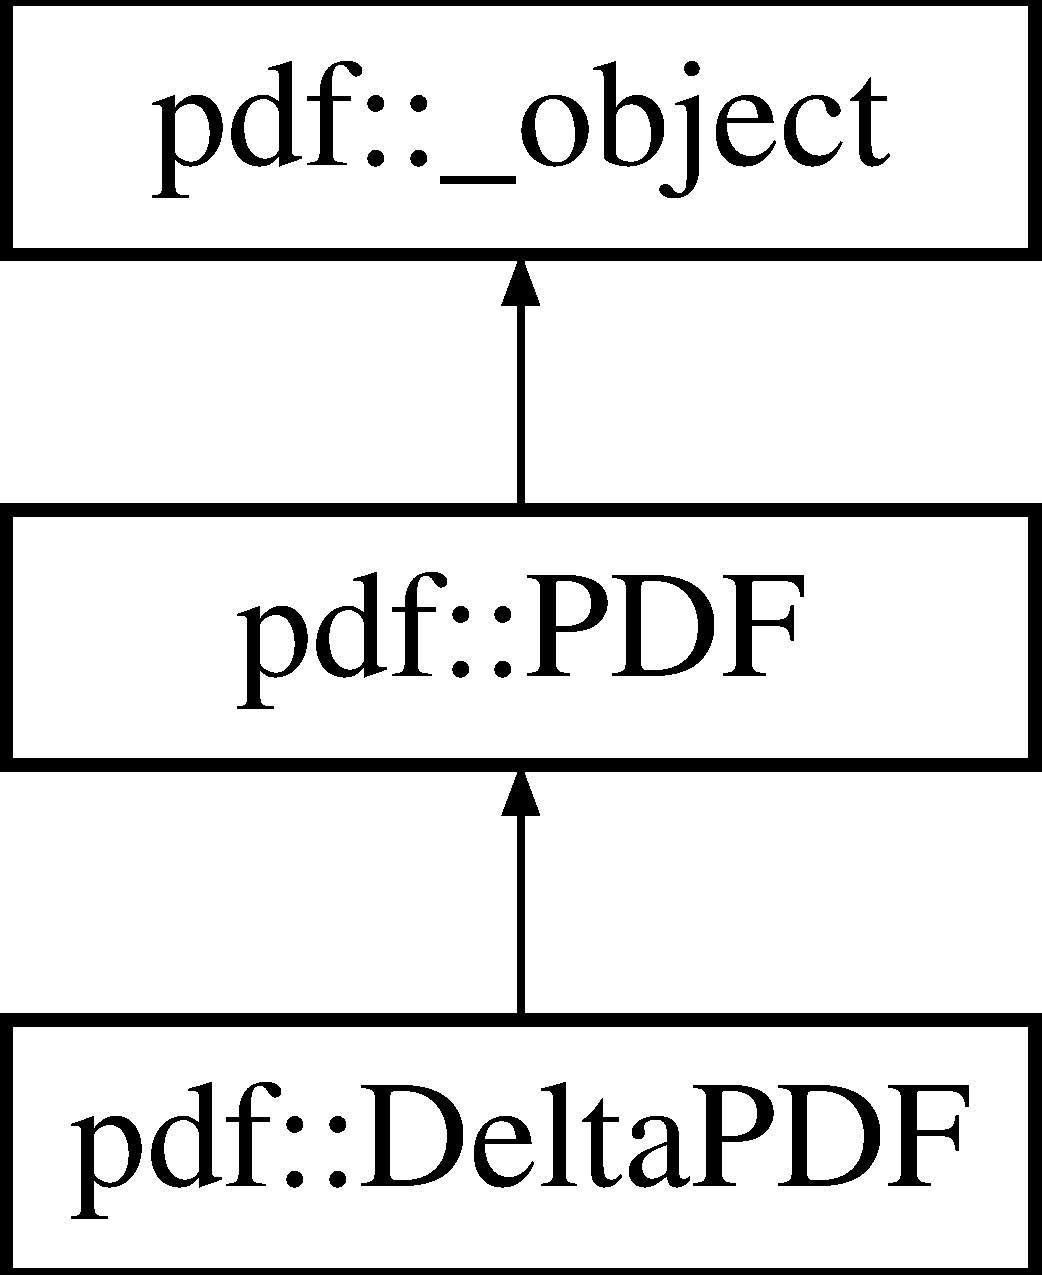
\includegraphics[height=3cm]{dc/d18/classpdf_1_1DeltaPDF}
\end{center}
\end{figure}
\subsection*{Public Member Functions}
\begin{DoxyCompactItemize}
\item 
\hypertarget{classpdf_1_1DeltaPDF_a6fdc3ea1145460c7872f078ae4c53f47}{
def {\bfseries \_\-\_\-init\_\-\_\-}}
\label{dc/d18/classpdf_1_1DeltaPDF_a6fdc3ea1145460c7872f078ae4c53f47}

\item 
\hypertarget{classpdf_1_1DeltaPDF_a39f58564645df6ada5bdfa96bdea11c9}{
def {\bfseries pdfVal}}
\label{dc/d18/classpdf_1_1DeltaPDF_a39f58564645df6ada5bdfa96bdea11c9}

\end{DoxyCompactItemize}
\subsection*{Public Attributes}
\begin{DoxyCompactItemize}
\item 
\hypertarget{classpdf_1_1DeltaPDF_a5060ddf377ac837c54c16a4f56bd10a6}{
{\bfseries this}}
\label{dc/d18/classpdf_1_1DeltaPDF_a5060ddf377ac837c54c16a4f56bd10a6}

\end{DoxyCompactItemize}


The documentation for this class was generated from the following file:\begin{DoxyCompactItemize}
\item 
src/pdf.py\end{DoxyCompactItemize}

\hypertarget{classDeltaPDF}{
\section{DeltaPDF Class Reference}
\label{dd/d98/classDeltaPDF}\index{DeltaPDF@{DeltaPDF}}
}


Evaluates delta \hyperlink{classPDF}{PDF} and stores values in a \hyperlink{classMatrix3D}{Matrix3D} object.  




{\ttfamily \#include $<$deltaPDF.h$>$}

Inheritance diagram for DeltaPDF:\begin{figure}[H]
\begin{center}
\leavevmode
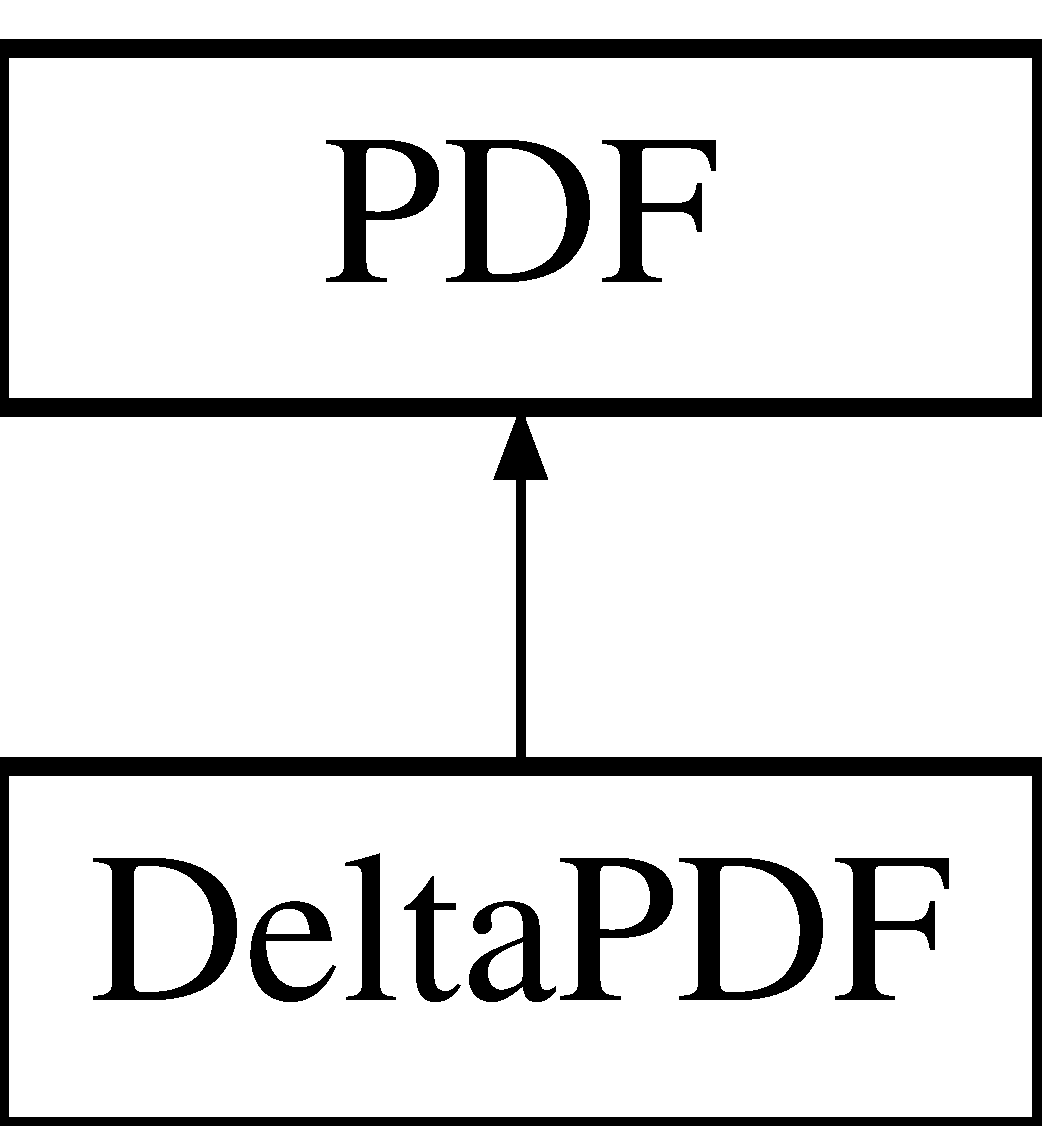
\includegraphics[height=2cm]{dd/d98/classDeltaPDF}
\end{center}
\end{figure}
\subsection*{Public Member Functions}
\begin{DoxyCompactItemize}
\item 
\hypertarget{classDeltaPDF_a6268a222dac459788d7a7589e0bec1c5}{
\hyperlink{classDeltaPDF_a6268a222dac459788d7a7589e0bec1c5}{DeltaPDF} (const double $\ast$Zmean, const int ZmeanPoints)}
\label{dd/d98/classDeltaPDF_a6268a222dac459788d7a7589e0bec1c5}

\begin{DoxyCompactList}\small\item\em Constructor. \item\end{DoxyCompactList}\item 
\hypertarget{classDeltaPDF_a9539ed9f2f24966af76b6bba4734b2be}{
\hyperlink{classDeltaPDF_a9539ed9f2f24966af76b6bba4734b2be}{$\sim$DeltaPDF} ()}
\label{dd/d98/classDeltaPDF_a9539ed9f2f24966af76b6bba4734b2be}

\begin{DoxyCompactList}\small\item\em Destructor. \item\end{DoxyCompactList}\item 
int \hyperlink{classDeltaPDF_a787e205c3bd8d4f95f7c528497e3a617}{pdfVal} (const double $\ast$Z, const int ZPoints, \hyperlink{classMatrix3D}{Matrix3D} $\ast$pdfValM)
\end{DoxyCompactItemize}


\subsection{Detailed Description}
Evaluates delta \hyperlink{classPDF}{PDF} and stores values in a \hyperlink{classMatrix3D}{Matrix3D} object. 

\subsection{Member Function Documentation}
\hypertarget{classDeltaPDF_a787e205c3bd8d4f95f7c528497e3a617}{
\index{DeltaPDF@{DeltaPDF}!pdfVal@{pdfVal}}
\index{pdfVal@{pdfVal}!DeltaPDF@{DeltaPDF}}
\subsubsection[{pdfVal}]{\setlength{\rightskip}{0pt plus 5cm}int DeltaPDF::pdfVal (const double $\ast$ {\em Z}, \/  const int {\em ZPoints}, \/  {\bf Matrix3D} $\ast$ {\em pdfValM})\hspace{0.3cm}{\ttfamily  \mbox{[}virtual\mbox{]}}}}
\label{dd/d98/classDeltaPDF_a787e205c3bd8d4f95f7c528497e3a617}
The Delta \hyperlink{classPDF}{PDF} uses statistics (means) to generate a \hyperlink{classPDF}{PDF}. The \hyperlink{classPDF}{PDF} values are stored in a \hyperlink{classMatrix3D}{Matrix3D} object: dim1 is the variance, dim2 is the mean, and dim3 are the data points.

\begin{DoxyVerb}
  
  INPUTS: 
  
  const double *Z           double arrray containing mixture fraction values coming from the files

  const int ZPoints         number of mixture fraction values in the Z array

  Matrix3D* pdfValm         the Matrix3D type container that stores the PDF values


  OUTPUT:

  int                       flag specifying whether or not the function succeeded
                             = 0: success
			    != 0: something went wrong

  \end{DoxyVerb}
 

Implements \hyperlink{classPDF}{PDF}.



The documentation for this class was generated from the following files:\begin{DoxyCompactItemize}
\item 
src/deltaPDF.h\item 
src/deltaPDF.cc\end{DoxyCompactItemize}

\hypertarget{classEndPointSlope}{
\section{EndPointSlope Class Reference}
\label{da/d7d/classEndPointSlope}\index{EndPointSlope@{EndPointSlope}}
}
Inheritance diagram for EndPointSlope:\begin{figure}[H]
\begin{center}
\leavevmode
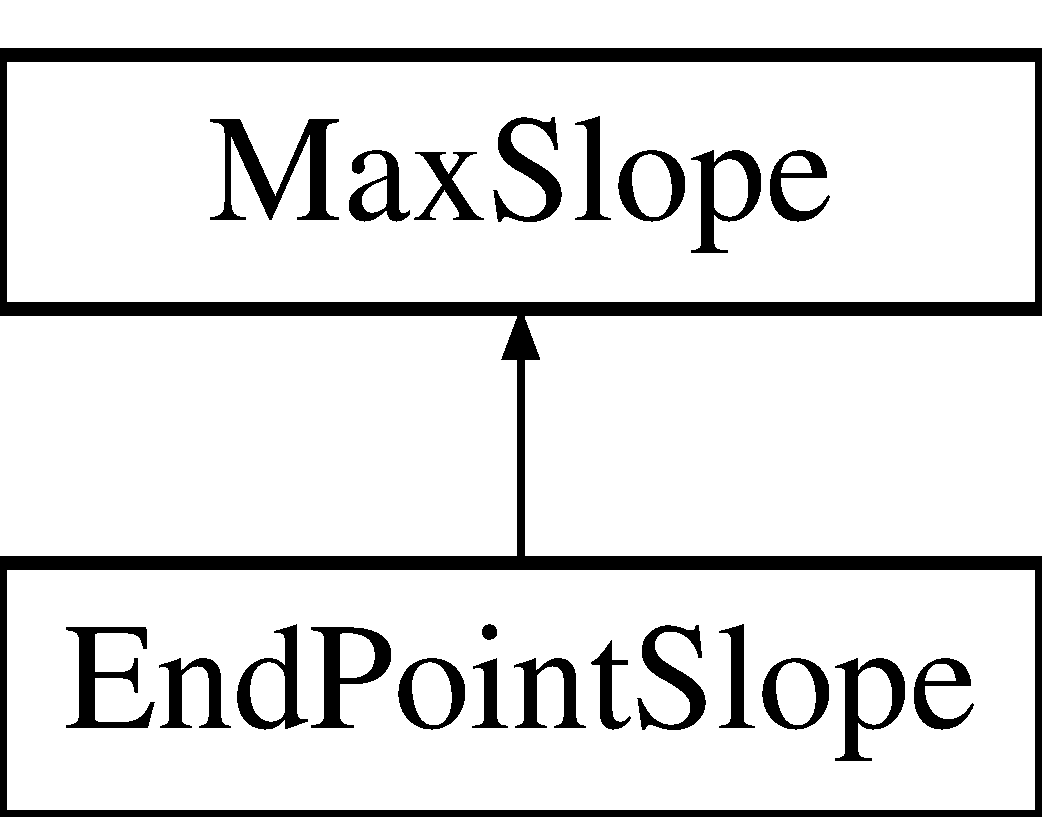
\includegraphics[height=2cm]{da/d7d/classEndPointSlope}
\end{center}
\end{figure}
\subsection*{Public Member Functions}
\begin{DoxyCompactItemize}
\item 
\hyperlink{classEndPointSlope_aa1c680c5137b40a465d2433e636892ce}{EndPointSlope} (const \hyperlink{classMatrix}{Matrix} \&progVar)
\begin{DoxyCompactList}\small\item\em Constructor. \item\end{DoxyCompactList}\item 
\hypertarget{classEndPointSlope_a37cf0a75d426b64fc50a8a76f45beb1f}{
\hyperlink{classEndPointSlope_a37cf0a75d426b64fc50a8a76f45beb1f}{$\sim$EndPointSlope} ()}
\label{da/d7d/classEndPointSlope_a37cf0a75d426b64fc50a8a76f45beb1f}

\begin{DoxyCompactList}\small\item\em Destructor. \item\end{DoxyCompactList}\item 
int \hyperlink{classEndPointSlope_a70417721fe8a60669a67d19a7855bef5}{MostMonotonic} (int $\ast$monoAry, const int ncols, const int col)
\begin{DoxyCompactList}\small\item\em Method to find the most monotonic progress variable. \item\end{DoxyCompactList}\end{DoxyCompactItemize}


\subsection{Constructor \& Destructor Documentation}
\hypertarget{classEndPointSlope_aa1c680c5137b40a465d2433e636892ce}{
\index{EndPointSlope@{EndPointSlope}!EndPointSlope@{EndPointSlope}}
\index{EndPointSlope@{EndPointSlope}!EndPointSlope@{EndPointSlope}}
\subsubsection[{EndPointSlope}]{\setlength{\rightskip}{0pt plus 5cm}EndPointSlope::EndPointSlope (const {\bf Matrix} \& {\em progVar})}}
\label{da/d7d/classEndPointSlope_aa1c680c5137b40a465d2433e636892ce}


Constructor. 

\hyperlink{classEndPointSlope}{EndPointSlope} is a class that determines the most monotonic progress variable with respect to temperature (or another specified column). It calculates the slope from the first and last endpoints of each progress variable column and selects the progress variable with the largest magnitude slope.

The slope is given by $ \frac{C_i(N) - C_i(1)}{N} $ 

\subsection{Member Function Documentation}
\hypertarget{classEndPointSlope_a70417721fe8a60669a67d19a7855bef5}{
\index{EndPointSlope@{EndPointSlope}!MostMonotonic@{MostMonotonic}}
\index{MostMonotonic@{MostMonotonic}!EndPointSlope@{EndPointSlope}}
\subsubsection[{MostMonotonic}]{\setlength{\rightskip}{0pt plus 5cm}int EndPointSlope::MostMonotonic (int $\ast$ {\em monoAry}, \/  const int {\em ncols}, \/  const int {\em col})\hspace{0.3cm}{\ttfamily  \mbox{[}virtual\mbox{]}}}}
\label{da/d7d/classEndPointSlope_a70417721fe8a60669a67d19a7855bef5}


Method to find the most monotonic progress variable. 

MostMonotonic calculates the slope of the best linear approximation for each progress variable which is strictly increasing or strictly decreasing. The output array monoAry must be of length ncols, where each cell holds a value of 3 if C is strictly monotonic and has the largest slope, 2 if C is strictly monotonic but does not have the largest slope, and 0 for non-\/monotonic C. col is the reference column.

\begin{DoxyVerb}
INPUTS:

int *monoAry       array containing integer flags that denote the monotonicity of candidate progress variables

const int ncols    number of columns of monoAry

const int col      the reference column

OUTPUT:

int                flag specifying whether or not the function succeeded 
                    = 0: success
		   != 0: something went wrong 
\end{DoxyVerb}
 

Implements \hyperlink{classMaxSlope_a494b1b1ae073d3b29fe7cdc023ce7861}{MaxSlope}.



The documentation for this class was generated from the following files:\begin{DoxyCompactItemize}
\item 
src/endpointslope.h\item 
src/endpointslope.cc\end{DoxyCompactItemize}

\hypertarget{classmaxslope_1_1EndPointSlope}{
\section{maxslope::EndPointSlope Class Reference}
\label{d5/d36/classmaxslope_1_1EndPointSlope}\index{maxslope::EndPointSlope@{maxslope::EndPointSlope}}
}
Inheritance diagram for maxslope::EndPointSlope:\begin{figure}[H]
\begin{center}
\leavevmode
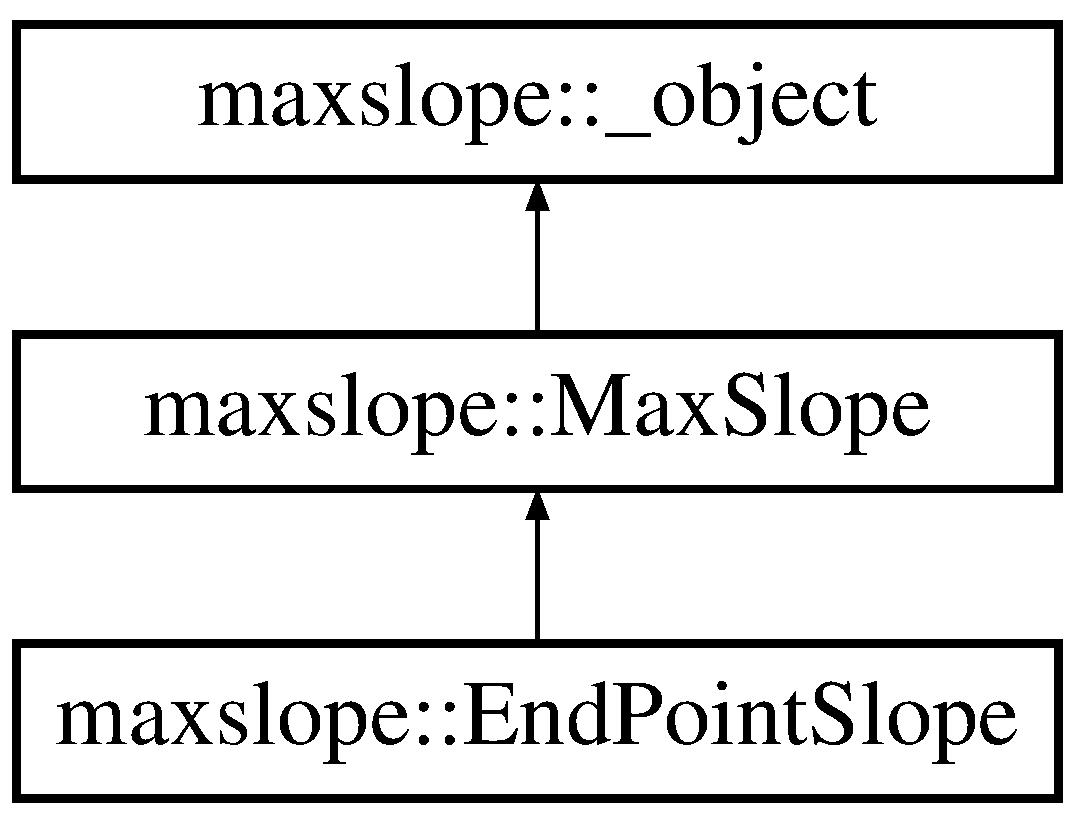
\includegraphics[height=3cm]{d5/d36/classmaxslope_1_1EndPointSlope}
\end{center}
\end{figure}
\subsection*{Public Member Functions}
\begin{DoxyCompactItemize}
\item 
\hypertarget{classmaxslope_1_1EndPointSlope_aa64ffcafb99bb6f9978a9037f14a18db}{
def {\bfseries \_\-\_\-init\_\-\_\-}}
\label{d5/d36/classmaxslope_1_1EndPointSlope_aa64ffcafb99bb6f9978a9037f14a18db}

\item 
\hypertarget{classmaxslope_1_1EndPointSlope_ac9ac444eccb64b1489ddf729975cb201}{
def {\bfseries MostMonotonic}}
\label{d5/d36/classmaxslope_1_1EndPointSlope_ac9ac444eccb64b1489ddf729975cb201}

\end{DoxyCompactItemize}
\subsection*{Public Attributes}
\begin{DoxyCompactItemize}
\item 
\hypertarget{classmaxslope_1_1EndPointSlope_ac09aca88eb1acd43cdfe6292862a3de1}{
{\bfseries this}}
\label{d5/d36/classmaxslope_1_1EndPointSlope_ac09aca88eb1acd43cdfe6292862a3de1}

\end{DoxyCompactItemize}


The documentation for this class was generated from the following file:\begin{DoxyCompactItemize}
\item 
src/maxslope.py\end{DoxyCompactItemize}

\hypertarget{classintegrator_1_1GLQuad}{
\section{integrator::GLQuad Class Reference}
\label{d0/de8/classintegrator_1_1GLQuad}\index{integrator::GLQuad@{integrator::GLQuad}}
}
Inheritance diagram for integrator::GLQuad:\begin{figure}[H]
\begin{center}
\leavevmode
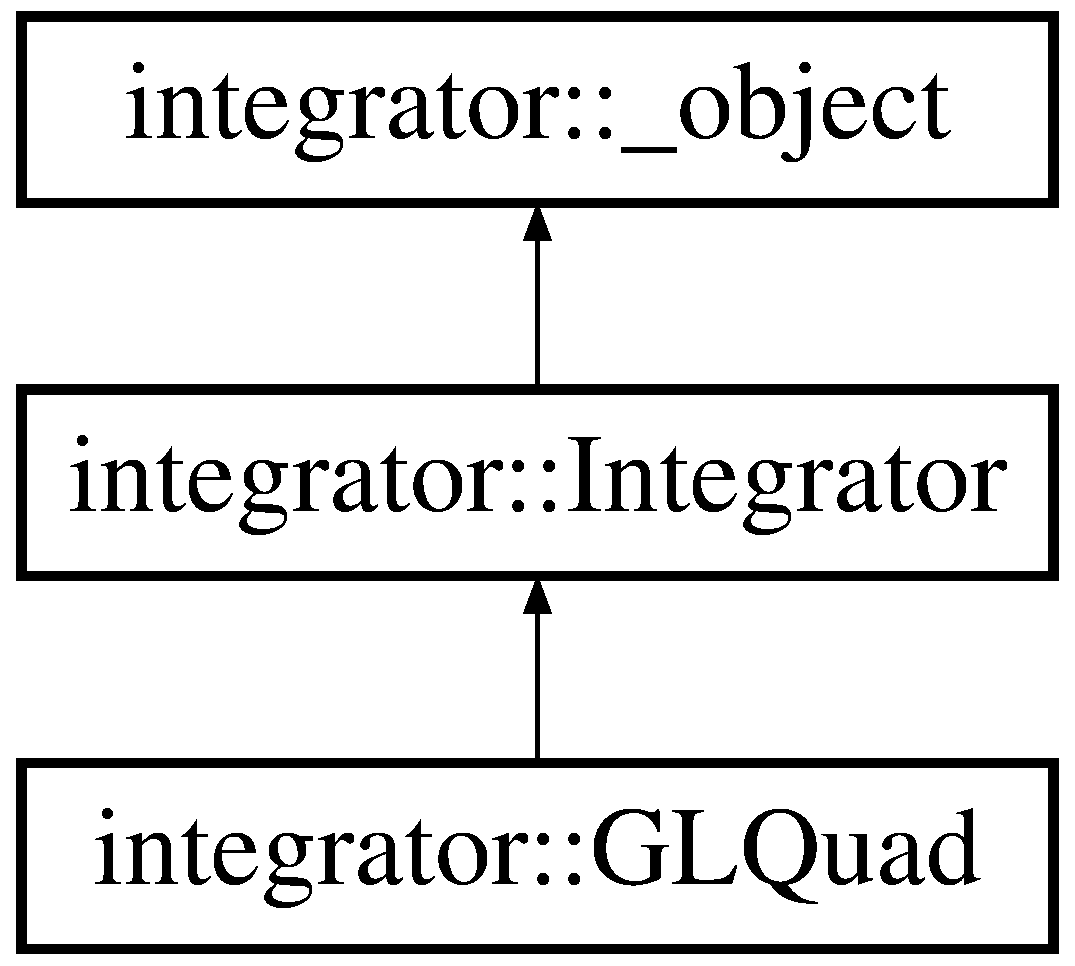
\includegraphics[height=3cm]{d0/de8/classintegrator_1_1GLQuad}
\end{center}
\end{figure}
\subsection*{Public Member Functions}
\begin{DoxyCompactItemize}
\item 
\hypertarget{classintegrator_1_1GLQuad_af1c5b397ad095a34096db39e83602ec9}{
def {\bfseries \_\-\_\-init\_\-\_\-}}
\label{d0/de8/classintegrator_1_1GLQuad_af1c5b397ad095a34096db39e83602ec9}

\item 
\hypertarget{classintegrator_1_1GLQuad_a85a93767e974c0890fe49e3811209cb4}{
def {\bfseries integrate}}
\label{d0/de8/classintegrator_1_1GLQuad_a85a93767e974c0890fe49e3811209cb4}

\end{DoxyCompactItemize}
\subsection*{Public Attributes}
\begin{DoxyCompactItemize}
\item 
\hypertarget{classintegrator_1_1GLQuad_a613996b0a038da751fa6cf2753d921cd}{
{\bfseries this}}
\label{d0/de8/classintegrator_1_1GLQuad_a613996b0a038da751fa6cf2753d921cd}

\end{DoxyCompactItemize}


The documentation for this class was generated from the following file:\begin{DoxyCompactItemize}
\item 
src/integrator.py\end{DoxyCompactItemize}

\hypertarget{classGLQuad}{
\section{GLQuad Class Reference}
\label{db/d06/classGLQuad}\index{GLQuad@{GLQuad}}
}


Calculates integral using Gauss-\/Legendre quadrature.  




{\ttfamily \#include $<$glquad.h$>$}

Inheritance diagram for GLQuad:\begin{figure}[H]
\begin{center}
\leavevmode
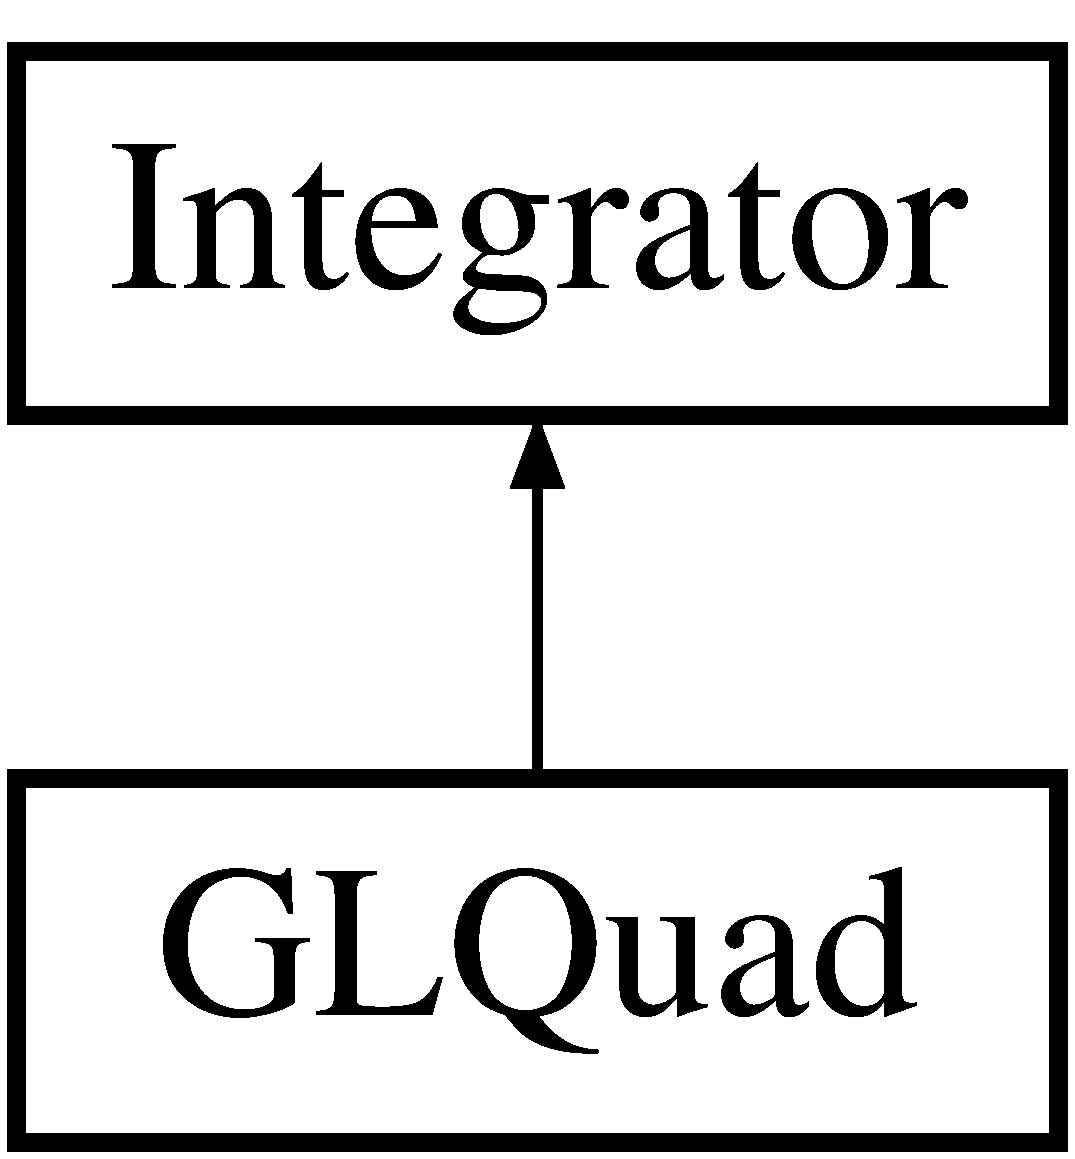
\includegraphics[height=2cm]{db/d06/classGLQuad}
\end{center}
\end{figure}
\subsection*{Public Member Functions}
\begin{DoxyCompactItemize}
\item 
\hyperlink{classGLQuad_a835d29af2507b6b2716794d3371d2ba8}{GLQuad} (int Nodes)
\begin{DoxyCompactList}\small\item\em Constructor. \item\end{DoxyCompactList}\item 
\hypertarget{classGLQuad_ad37beb73af53a94ca95ee8eddfe207ab}{
\hyperlink{classGLQuad_ad37beb73af53a94ca95ee8eddfe207ab}{$\sim$GLQuad} ()}
\label{db/d06/classGLQuad_ad37beb73af53a94ca95ee8eddfe207ab}

\begin{DoxyCompactList}\small\item\em Destructor. \item\end{DoxyCompactList}\item 
double \hyperlink{classGLQuad_a951e36d849cfadc749a62218212802b6}{integrate} (const double $\ast$integrand, const double $\ast$Z, const int ZPoints)
\begin{DoxyCompactList}\small\item\em Integration using Gauss-\/Legendre quadrature. \item\end{DoxyCompactList}\end{DoxyCompactItemize}


\subsection{Detailed Description}
Calculates integral using Gauss-\/Legendre quadrature. \hyperlink{classGLQuad}{GLQuad} takes in an array (the integrand) and returns the integral of that array using Gauss-\/Legendre quadrature. Abscissa are calculated using the external library AlgLib. 

\subsection{Constructor \& Destructor Documentation}
\hypertarget{classGLQuad_a835d29af2507b6b2716794d3371d2ba8}{
\index{GLQuad@{GLQuad}!GLQuad@{GLQuad}}
\index{GLQuad@{GLQuad}!GLQuad@{GLQuad}}
\subsubsection[{GLQuad}]{\setlength{\rightskip}{0pt plus 5cm}GLQuad::GLQuad (int {\em Nodes})}}
\label{db/d06/classGLQuad_a835d29af2507b6b2716794d3371d2ba8}


Constructor. 

Coordinates of abcissas are calculated in this function.

INPUTS:

const int Nodes number of abcissa

OUTPUT:

No particular output objects. Abcissas and weights are stored in x\_\- and w\_\- objects, respectively. 

\subsection{Member Function Documentation}
\hypertarget{classGLQuad_a951e36d849cfadc749a62218212802b6}{
\index{GLQuad@{GLQuad}!integrate@{integrate}}
\index{integrate@{integrate}!GLQuad@{GLQuad}}
\subsubsection[{integrate}]{\setlength{\rightskip}{0pt plus 5cm}double GLQuad::integrate (const double $\ast$ {\em integrand}, \/  const double $\ast$ {\em Z}, \/  const int {\em ZPoints})\hspace{0.3cm}{\ttfamily  \mbox{[}virtual\mbox{]}}}}
\label{db/d06/classGLQuad_a951e36d849cfadc749a62218212802b6}


Integration using Gauss-\/Legendre quadrature. 

Gauss-\/Legendre quadrature is applied to integrate a given integrand over a given double array, Z. Abcissas and weights are created during the execution of the constructor. The default number of nodes is 20, the number of nodes for the quadrature can be modified from the input file

\begin{DoxyVerb}
  INPUTS:

  const double *integrand            array that contains function values to be integrated

  const double *Z                    array that contains the mixture fraction values which the integrand will be integrated over

  const int ZPoints                  number of values, size of the integrand and Z containers
  
  OUTPUT:

  double                             result of the integration

  \end{DoxyVerb}
 

Implements \hyperlink{classIntegrator_a89fbef2f7923ce4e2c979b2ff1d1f4ac}{Integrator}.



The documentation for this class was generated from the following files:\begin{DoxyCompactItemize}
\item 
src/glquad.h\item 
src/glquad.cc\end{DoxyCompactItemize}

\hypertarget{classHermiteInterp}{
\section{HermiteInterp Class Reference}
\label{dd/d1b/classHermiteInterp}\index{HermiteInterp@{HermiteInterp}}
}
Inheritance diagram for HermiteInterp:\begin{figure}[H]
\begin{center}
\leavevmode
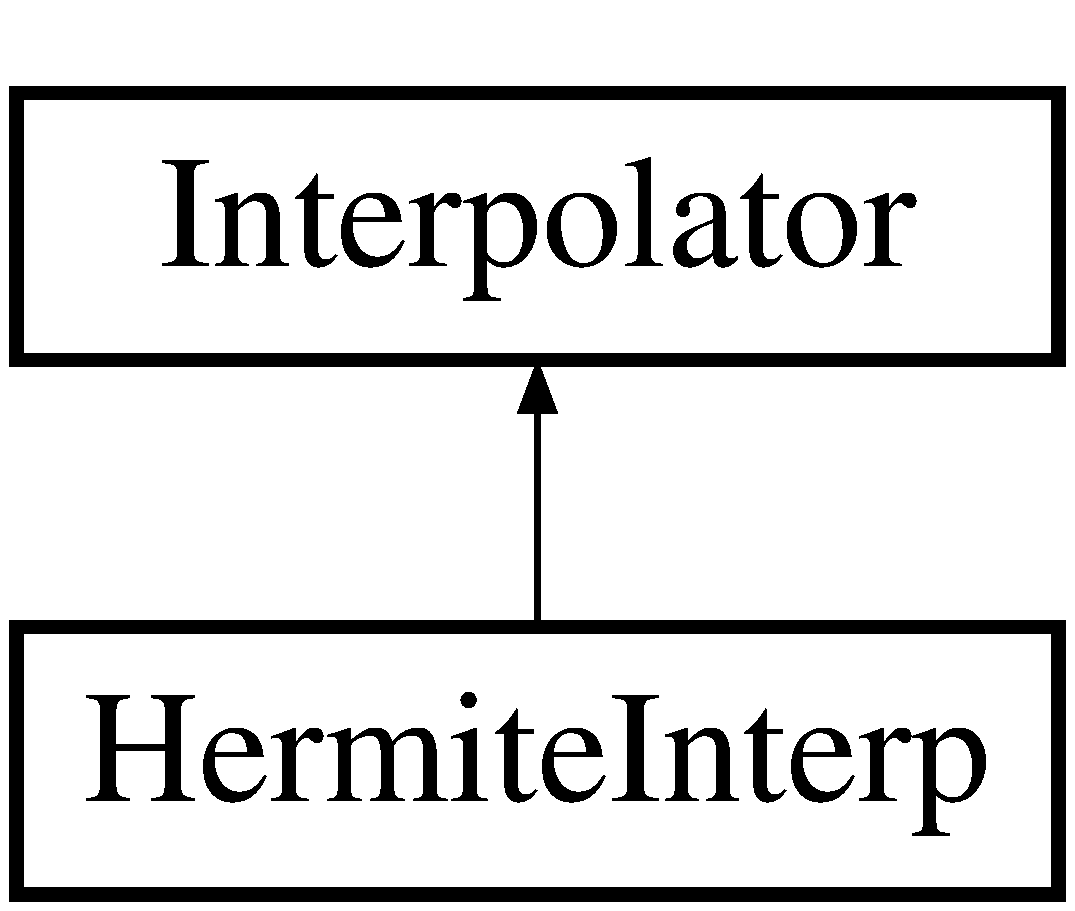
\includegraphics[height=2cm]{dd/d1b/classHermiteInterp}
\end{center}
\end{figure}
\subsection*{Public Member Functions}
\begin{DoxyCompactItemize}
\item 
\hypertarget{classHermiteInterp_a3c50ee042f7708addc2ac2afadbd5b1b}{
\hyperlink{classHermiteInterp_a3c50ee042f7708addc2ac2afadbd5b1b}{HermiteInterp} ()}
\label{dd/d1b/classHermiteInterp_a3c50ee042f7708addc2ac2afadbd5b1b}

\begin{DoxyCompactList}\small\item\em Constructor. \item\end{DoxyCompactList}\item 
\hypertarget{classHermiteInterp_a458bdb7a9130ec7b7f018babe15bf058}{
\hyperlink{classHermiteInterp_a458bdb7a9130ec7b7f018babe15bf058}{$\sim$HermiteInterp} ()}
\label{dd/d1b/classHermiteInterp_a458bdb7a9130ec7b7f018babe15bf058}

\begin{DoxyCompactList}\small\item\em Destructor. \item\end{DoxyCompactList}\item 
int \hyperlink{classHermiteInterp_a3de30c92f2e22b207a32b221d4a09ff9}{Interp} (const \hyperlink{classMatrix}{Matrix} $\ast$matin, int col, double ival, double $\ast$vecout, int cols)
\begin{DoxyCompactList}\small\item\em Hermite spline interpolation function. \item\end{DoxyCompactList}\end{DoxyCompactItemize}


\subsection{Member Function Documentation}
\hypertarget{classHermiteInterp_a3de30c92f2e22b207a32b221d4a09ff9}{
\index{HermiteInterp@{HermiteInterp}!Interp@{Interp}}
\index{Interp@{Interp}!HermiteInterp@{HermiteInterp}}
\subsubsection[{Interp}]{\setlength{\rightskip}{0pt plus 5cm}int HermiteInterp::Interp (const {\bf Matrix} $\ast$ {\em matin}, \/  int {\em col}, \/  double {\em ival}, \/  double $\ast$ {\em vecout}, \/  int {\em cols})\hspace{0.3cm}{\ttfamily  \mbox{[}virtual\mbox{]}}}}
\label{dd/d1b/classHermiteInterp_a3de30c92f2e22b207a32b221d4a09ff9}


Hermite spline interpolation function. 

This function takes in a 2D matrix of data and interpolates an entire row from it using a hermite spline interpolator. Each column of the matrix is treated as a variable, with a specified column being the independent variable. The input data is assumed to be sorted

\begin{DoxyVerb}
  INPUTS:

  const Matrix *matin    pointer to a Matrix object. This is the input data.

  int col                integer specifying which column of the input Matrix is the independent
                         variable

  double ival            value at which to interpolate

  double *vecout         pointer to an array which contains the interpolated row. This array has
                         the same number of columns as the input Matrix.

  int cols               number of columns of matin/vecout


  OUTPUTS:

  int                    flag specifying whether or not the function succeeded
                         = 0: success
			 = 1: extrapolation attempted

\end{DoxyVerb}
 

Implements \hyperlink{classInterpolator_a2238defccb009047f624bda33cc47c73}{Interpolator}.



The documentation for this class was generated from the following files:\begin{DoxyCompactItemize}
\item 
src/hermiteinterp.h\item 
src/hermiteinterp.cc\end{DoxyCompactItemize}

\hypertarget{classinterpolator_1_1HermiteInterp}{
\section{interpolator::HermiteInterp Class Reference}
\label{db/dc6/classinterpolator_1_1HermiteInterp}\index{interpolator::HermiteInterp@{interpolator::HermiteInterp}}
}
Inheritance diagram for interpolator::HermiteInterp:\begin{figure}[H]
\begin{center}
\leavevmode
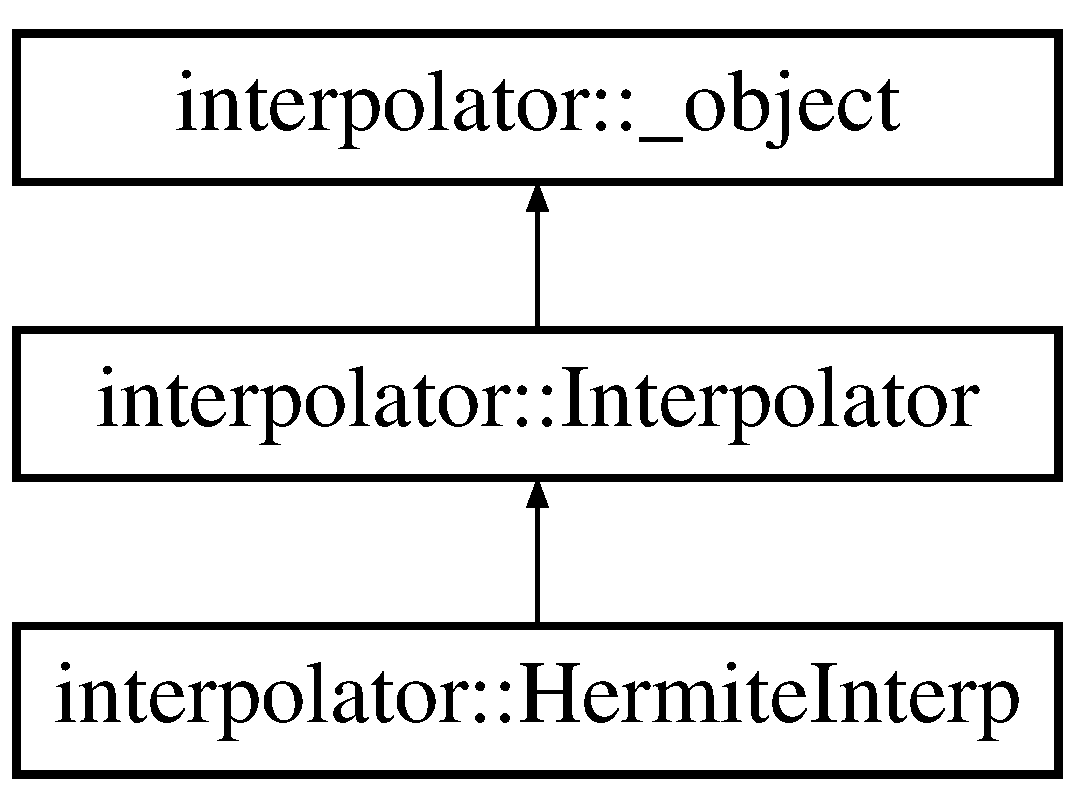
\includegraphics[height=3cm]{db/dc6/classinterpolator_1_1HermiteInterp}
\end{center}
\end{figure}
\subsection*{Public Member Functions}
\begin{DoxyCompactItemize}
\item 
\hypertarget{classinterpolator_1_1HermiteInterp_a1594626eba5f17c46258c300bbd4c20e}{
def {\bfseries \_\-\_\-init\_\-\_\-}}
\label{db/dc6/classinterpolator_1_1HermiteInterp_a1594626eba5f17c46258c300bbd4c20e}

\item 
\hypertarget{classinterpolator_1_1HermiteInterp_a58621e7cc00225ca1f755c0d1c6e16dd}{
def {\bfseries Interp}}
\label{db/dc6/classinterpolator_1_1HermiteInterp_a58621e7cc00225ca1f755c0d1c6e16dd}

\end{DoxyCompactItemize}
\subsection*{Public Attributes}
\begin{DoxyCompactItemize}
\item 
\hypertarget{classinterpolator_1_1HermiteInterp_af681d0746a0c7c00310b4abb044e99a8}{
{\bfseries this}}
\label{db/dc6/classinterpolator_1_1HermiteInterp_af681d0746a0c7c00310b4abb044e99a8}

\end{DoxyCompactItemize}


The documentation for this class was generated from the following file:\begin{DoxyCompactItemize}
\item 
src/interpolator.py\end{DoxyCompactItemize}

\hypertarget{classIntegrator}{
\section{Integrator Class Reference}
\label{da/d05/classIntegrator}\index{Integrator@{Integrator}}
}
Inheritance diagram for Integrator:\begin{figure}[H]
\begin{center}
\leavevmode
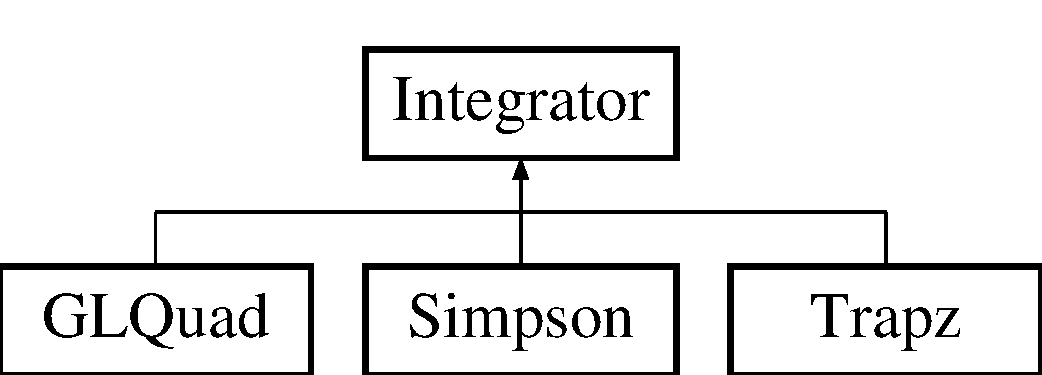
\includegraphics[height=2cm]{da/d05/classIntegrator}
\end{center}
\end{figure}
\subsection*{Public Member Functions}
\begin{DoxyCompactItemize}
\item 
\hypertarget{classIntegrator_a89fbef2f7923ce4e2c979b2ff1d1f4ac}{
virtual double \hyperlink{classIntegrator_a89fbef2f7923ce4e2c979b2ff1d1f4ac}{integrate} (const double $\ast$integrand, const double $\ast$Z, const int ZPoints)=0}
\label{da/d05/classIntegrator_a89fbef2f7923ce4e2c979b2ff1d1f4ac}

\begin{DoxyCompactList}\small\item\em Virtual function to be inherited by each integration algorithm to integrate the given data set. \item\end{DoxyCompactList}\end{DoxyCompactItemize}


The documentation for this class was generated from the following file:\begin{DoxyCompactItemize}
\item 
src/integrator.h\end{DoxyCompactItemize}

\hypertarget{classintegrator_1_1Integrator}{
\section{integrator::Integrator Class Reference}
\label{dc/da1/classintegrator_1_1Integrator}\index{integrator::Integrator@{integrator::Integrator}}
}
Inheritance diagram for integrator::Integrator:\begin{figure}[H]
\begin{center}
\leavevmode
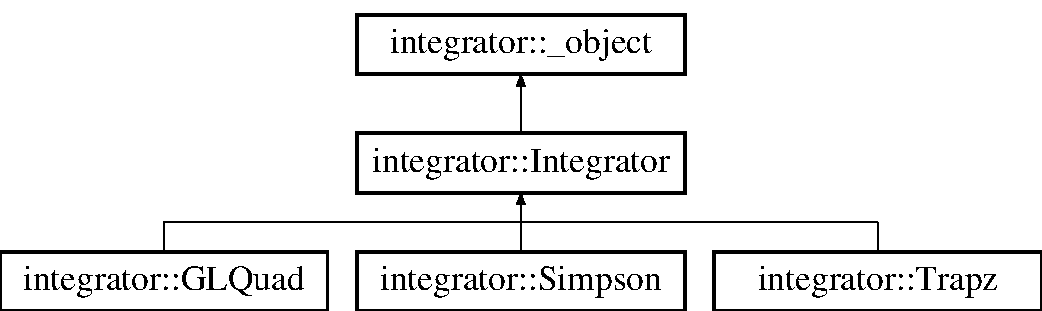
\includegraphics[height=3cm]{dc/da1/classintegrator_1_1Integrator}
\end{center}
\end{figure}
\subsection*{Public Member Functions}
\begin{DoxyCompactItemize}
\item 
\hypertarget{classintegrator_1_1Integrator_a973f474b13cde1d131d4a187b6b9f498}{
def {\bfseries \_\-\_\-init\_\-\_\-}}
\label{dc/da1/classintegrator_1_1Integrator_a973f474b13cde1d131d4a187b6b9f498}

\item 
\hypertarget{classintegrator_1_1Integrator_a7ab4e9c4f500e5c1020508e160237e0e}{
def {\bfseries integrate}}
\label{dc/da1/classintegrator_1_1Integrator_a7ab4e9c4f500e5c1020508e160237e0e}

\end{DoxyCompactItemize}


The documentation for this class was generated from the following file:\begin{DoxyCompactItemize}
\item 
src/integrator.py\end{DoxyCompactItemize}

\hypertarget{classInterpolator}{
\section{Interpolator Class Reference}
\label{d3/df3/classInterpolator}\index{Interpolator@{Interpolator}}
}
Inheritance diagram for Interpolator:\begin{figure}[H]
\begin{center}
\leavevmode
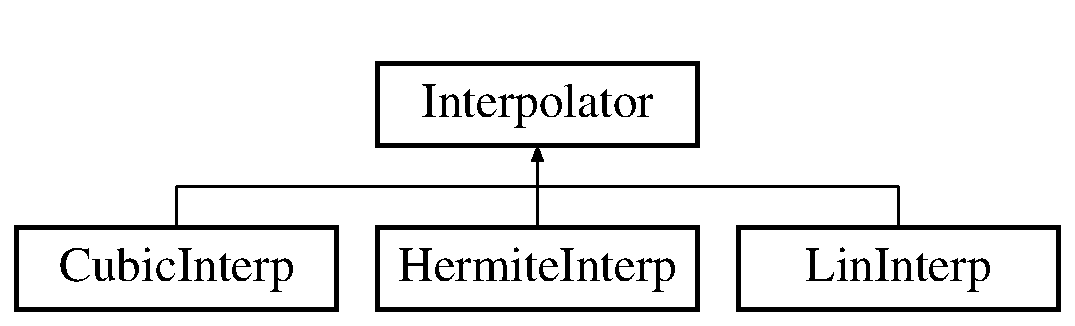
\includegraphics[height=2cm]{d3/df3/classInterpolator}
\end{center}
\end{figure}
\subsection*{Public Member Functions}
\begin{DoxyCompactItemize}
\item 
\hypertarget{classInterpolator_a2238defccb009047f624bda33cc47c73}{
virtual int \hyperlink{classInterpolator_a2238defccb009047f624bda33cc47c73}{Interp} (const \hyperlink{classMatrix}{Matrix} $\ast$matin, int col, double ival, double $\ast$vecout, int cols)=0}
\label{d3/df3/classInterpolator_a2238defccb009047f624bda33cc47c73}

\begin{DoxyCompactList}\small\item\em Virtual function to be inherited by each interpolation algorithm to interpolate the given data. \item\end{DoxyCompactList}\end{DoxyCompactItemize}


The documentation for this class was generated from the following file:\begin{DoxyCompactItemize}
\item 
src/interpolator.h\end{DoxyCompactItemize}

\hypertarget{classinterpolator_1_1Interpolator}{
\section{interpolator::Interpolator Class Reference}
\label{db/dc2/classinterpolator_1_1Interpolator}\index{interpolator::Interpolator@{interpolator::Interpolator}}
}
Inheritance diagram for interpolator::Interpolator:\begin{figure}[H]
\begin{center}
\leavevmode
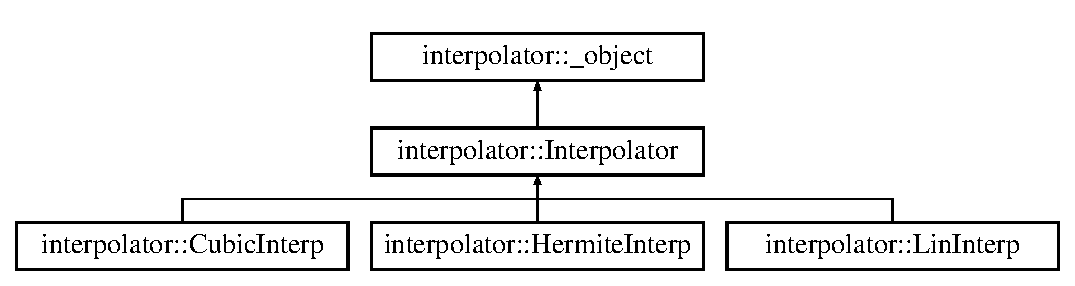
\includegraphics[height=3cm]{db/dc2/classinterpolator_1_1Interpolator}
\end{center}
\end{figure}
\subsection*{Public Member Functions}
\begin{DoxyCompactItemize}
\item 
\hypertarget{classinterpolator_1_1Interpolator_af19c595578ba5c3e8caad32812464594}{
def {\bfseries \_\-\_\-init\_\-\_\-}}
\label{db/dc2/classinterpolator_1_1Interpolator_af19c595578ba5c3e8caad32812464594}

\item 
\hypertarget{classinterpolator_1_1Interpolator_afff6d180a690fa9939f12ceb969a0a4e}{
def {\bfseries Interp}}
\label{db/dc2/classinterpolator_1_1Interpolator_afff6d180a690fa9939f12ceb969a0a4e}

\end{DoxyCompactItemize}


The documentation for this class was generated from the following file:\begin{DoxyCompactItemize}
\item 
src/interpolator.py\end{DoxyCompactItemize}

\hypertarget{classLeastNonMono}{
\section{LeastNonMono Class Reference}
\label{d9/da9/classLeastNonMono}\index{LeastNonMono@{LeastNonMono}}
}
Inheritance diagram for LeastNonMono:\begin{figure}[H]
\begin{center}
\leavevmode
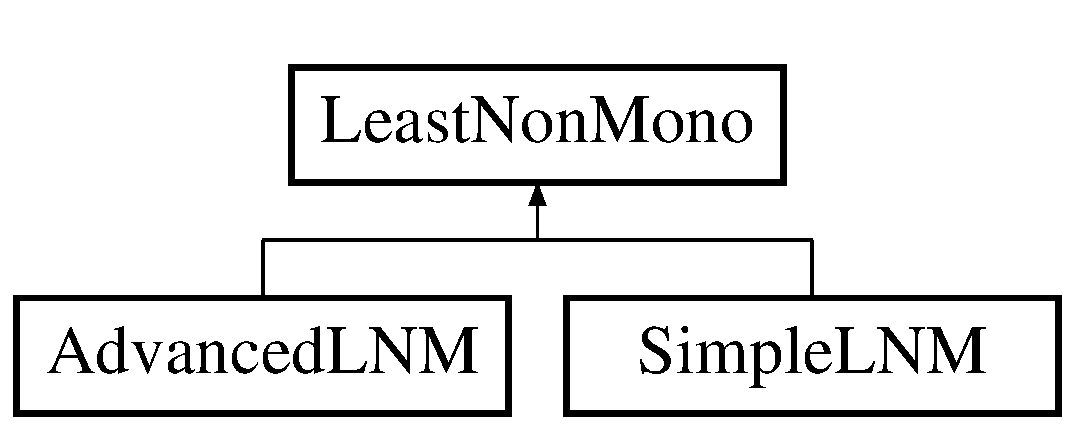
\includegraphics[height=2cm]{d9/da9/classLeastNonMono}
\end{center}
\end{figure}
\subsection*{Public Member Functions}
\begin{DoxyCompactItemize}
\item 
\hypertarget{classLeastNonMono_a239cbd7836950dc7c758138c4db00d0c}{
virtual int \hyperlink{classLeastNonMono_a239cbd7836950dc7c758138c4db00d0c}{LeastNonMonotonic} (int $\ast$monoAry, const int ncols, const int col)=0}
\label{d9/da9/classLeastNonMono_a239cbd7836950dc7c758138c4db00d0c}

\begin{DoxyCompactList}\small\item\em Virtual function to be inherited by each monotonicity cheking algorithm to determine the least non-\/monotonic progress variable. \item\end{DoxyCompactList}\end{DoxyCompactItemize}


The documentation for this class was generated from the following file:\begin{DoxyCompactItemize}
\item 
src/leastnonmono.h\end{DoxyCompactItemize}

\hypertarget{classleastnonmono_1_1LeastNonMono}{
\section{leastnonmono::LeastNonMono Class Reference}
\label{da/d81/classleastnonmono_1_1LeastNonMono}\index{leastnonmono::LeastNonMono@{leastnonmono::LeastNonMono}}
}
Inheritance diagram for leastnonmono::LeastNonMono:\begin{figure}[H]
\begin{center}
\leavevmode
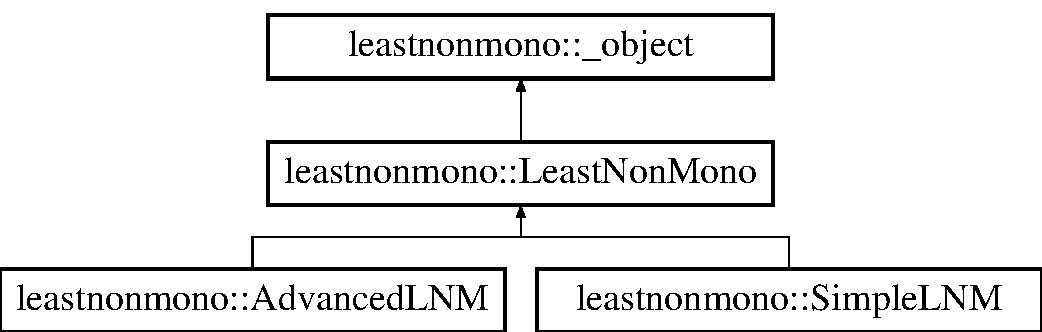
\includegraphics[height=3cm]{da/d81/classleastnonmono_1_1LeastNonMono}
\end{center}
\end{figure}
\subsection*{Public Member Functions}
\begin{DoxyCompactItemize}
\item 
\hypertarget{classleastnonmono_1_1LeastNonMono_ad27a656979919a3cf13907470b53fc2d}{
def {\bfseries \_\-\_\-init\_\-\_\-}}
\label{da/d81/classleastnonmono_1_1LeastNonMono_ad27a656979919a3cf13907470b53fc2d}

\item 
\hypertarget{classleastnonmono_1_1LeastNonMono_ab1899f44db61835de8d8f819a07bf07d}{
def {\bfseries LeastNonMonotonic}}
\label{da/d81/classleastnonmono_1_1LeastNonMono_ab1899f44db61835de8d8f819a07bf07d}

\end{DoxyCompactItemize}


The documentation for this class was generated from the following file:\begin{DoxyCompactItemize}
\item 
src/leastnonmono.py\end{DoxyCompactItemize}

\hypertarget{classinterpolator_1_1LinInterp}{
\section{interpolator::LinInterp Class Reference}
\label{df/d7e/classinterpolator_1_1LinInterp}\index{interpolator::LinInterp@{interpolator::LinInterp}}
}
Inheritance diagram for interpolator::LinInterp:\begin{figure}[H]
\begin{center}
\leavevmode
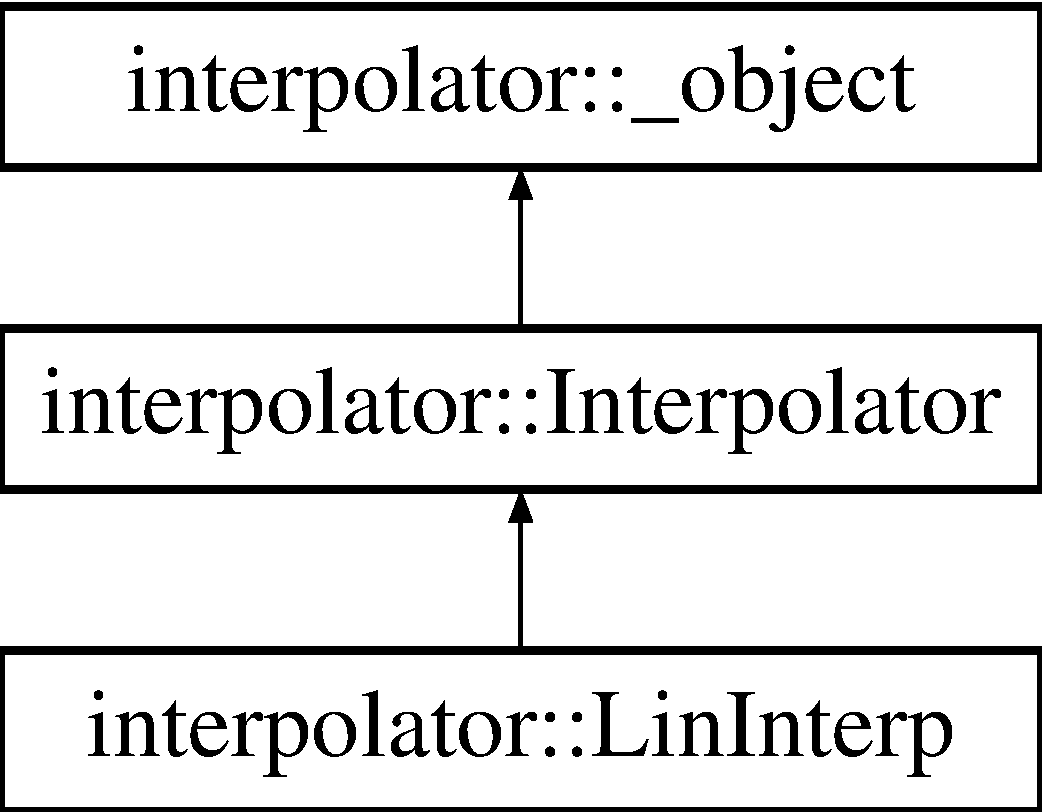
\includegraphics[height=3cm]{df/d7e/classinterpolator_1_1LinInterp}
\end{center}
\end{figure}
\subsection*{Public Member Functions}
\begin{DoxyCompactItemize}
\item 
\hypertarget{classinterpolator_1_1LinInterp_aa9f273599a1e0558c90d0483e9d05e73}{
def {\bfseries \_\-\_\-init\_\-\_\-}}
\label{df/d7e/classinterpolator_1_1LinInterp_aa9f273599a1e0558c90d0483e9d05e73}

\item 
\hypertarget{classinterpolator_1_1LinInterp_a397581a63f3406289ffddb9fbc83538b}{
def {\bfseries Interp}}
\label{df/d7e/classinterpolator_1_1LinInterp_a397581a63f3406289ffddb9fbc83538b}

\end{DoxyCompactItemize}
\subsection*{Public Attributes}
\begin{DoxyCompactItemize}
\item 
\hypertarget{classinterpolator_1_1LinInterp_a3512f4d431e4c275621dc18956cde58a}{
{\bfseries this}}
\label{df/d7e/classinterpolator_1_1LinInterp_a3512f4d431e4c275621dc18956cde58a}

\end{DoxyCompactItemize}


The documentation for this class was generated from the following file:\begin{DoxyCompactItemize}
\item 
src/interpolator.py\end{DoxyCompactItemize}

\hypertarget{classLinInterp}{
\section{LinInterp Class Reference}
\label{d8/dee/classLinInterp}\index{LinInterp@{LinInterp}}
}
Inheritance diagram for LinInterp:\begin{figure}[H]
\begin{center}
\leavevmode
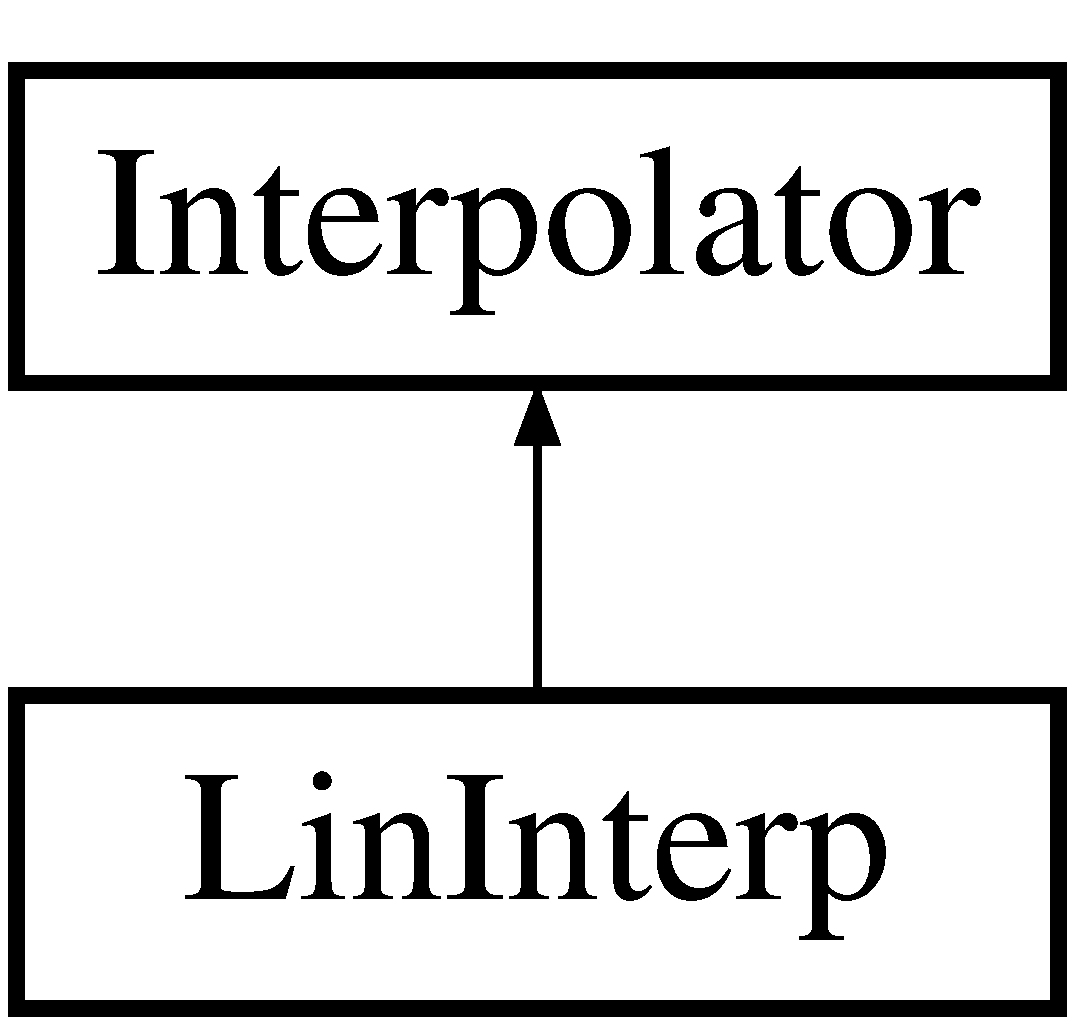
\includegraphics[height=2cm]{d8/dee/classLinInterp}
\end{center}
\end{figure}
\subsection*{Public Member Functions}
\begin{DoxyCompactItemize}
\item 
\hypertarget{classLinInterp_a56a58464dae6196cc671749133f1de12}{
\hyperlink{classLinInterp_a56a58464dae6196cc671749133f1de12}{LinInterp} ()}
\label{d8/dee/classLinInterp_a56a58464dae6196cc671749133f1de12}

\begin{DoxyCompactList}\small\item\em Constructor. \item\end{DoxyCompactList}\item 
\hypertarget{classLinInterp_a301177227b3013bcf9ea45e1c66fc468}{
\hyperlink{classLinInterp_a301177227b3013bcf9ea45e1c66fc468}{$\sim$LinInterp} ()}
\label{d8/dee/classLinInterp_a301177227b3013bcf9ea45e1c66fc468}

\begin{DoxyCompactList}\small\item\em Destructor. \item\end{DoxyCompactList}\item 
int \hyperlink{classLinInterp_a26aeb03c387bf5c8ea5db0ed111b5cd7}{Interp} (const \hyperlink{classMatrix}{Matrix} $\ast$matin, int col, double ival, double $\ast$vecout, int cols)
\begin{DoxyCompactList}\small\item\em Linear interpolation function. \item\end{DoxyCompactList}\end{DoxyCompactItemize}


\subsection{Member Function Documentation}
\hypertarget{classLinInterp_a26aeb03c387bf5c8ea5db0ed111b5cd7}{
\index{LinInterp@{LinInterp}!Interp@{Interp}}
\index{Interp@{Interp}!LinInterp@{LinInterp}}
\subsubsection[{Interp}]{\setlength{\rightskip}{0pt plus 5cm}int LinInterp::Interp (const {\bf Matrix} $\ast$ {\em matin}, \/  int {\em col}, \/  double {\em ival}, \/  double $\ast$ {\em vecout}, \/  int {\em cols})\hspace{0.3cm}{\ttfamily  \mbox{[}virtual\mbox{]}}}}
\label{d8/dee/classLinInterp_a26aeb03c387bf5c8ea5db0ed111b5cd7}


Linear interpolation function. 

This function takes in a 2D matrix of data and interpolates an entire row from it using a linear interpolator. Each column of the matrix is treated as a variable, with a specified column being the independent variable. The input data is not assumed to be sorted.

\begin{DoxyVerb}
  INPUTS:

  const Matrix *matin    pointer to a Matrix object. This is the input data.

  int col                integer specifying which column of the input Matrix is the independent 
                         variable

  double ival            value at which to interpolate

  double *vecout         pointer to an array which contains the interpolated row. This array has
                         the same number of columns as the input Matrix.

  int cols               number of columns of matin/vecout


  OUTPUTS:

  int                    flag specifying whether or not the function succeeded
                         = 0: success
			 = 1: extrapolation attempted
\end{DoxyVerb}
 

Implements \hyperlink{classInterpolator_a2238defccb009047f624bda33cc47c73}{Interpolator}.



The documentation for this class was generated from the following files:\begin{DoxyCompactItemize}
\item 
src/lininterp.h\item 
src/lininterp.cc\end{DoxyCompactItemize}

\hypertarget{classmaxslope_1_1LinRegression}{
\section{maxslope::LinRegression Class Reference}
\label{d4/dbe/classmaxslope_1_1LinRegression}\index{maxslope::LinRegression@{maxslope::LinRegression}}
}
Inheritance diagram for maxslope::LinRegression:\begin{figure}[H]
\begin{center}
\leavevmode
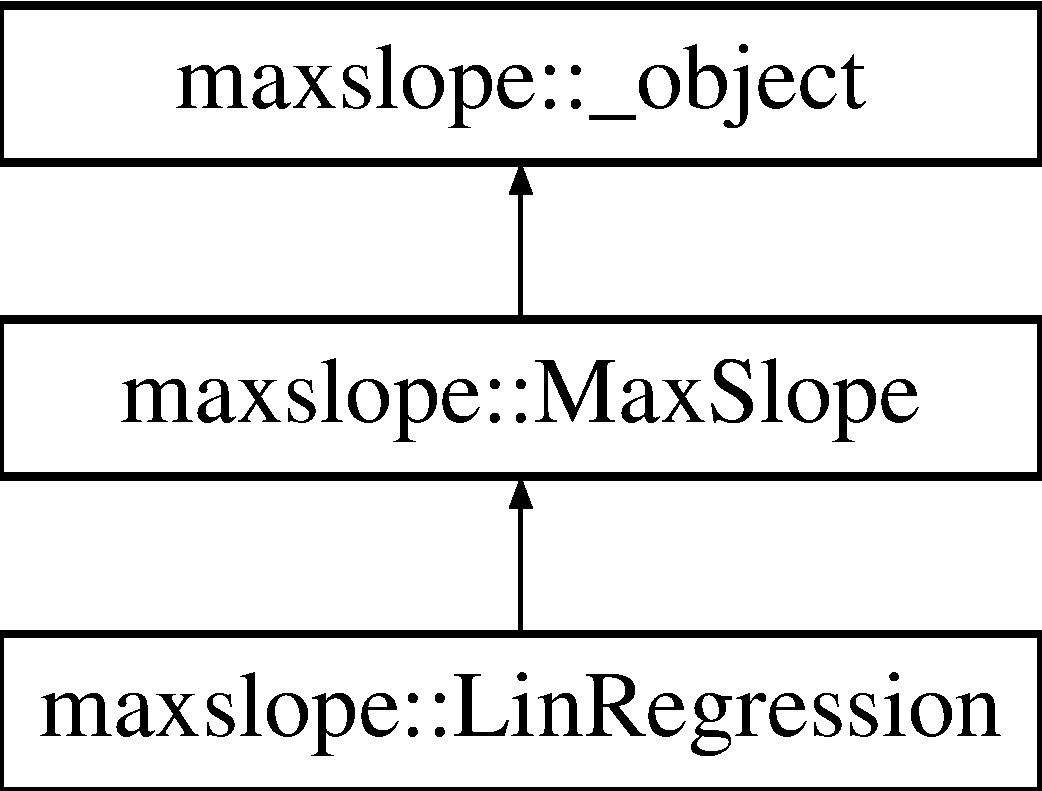
\includegraphics[height=3cm]{d4/dbe/classmaxslope_1_1LinRegression}
\end{center}
\end{figure}
\subsection*{Public Member Functions}
\begin{DoxyCompactItemize}
\item 
\hypertarget{classmaxslope_1_1LinRegression_ab45de3d79a109d5e052e219a102dbeec}{
def {\bfseries \_\-\_\-init\_\-\_\-}}
\label{d4/dbe/classmaxslope_1_1LinRegression_ab45de3d79a109d5e052e219a102dbeec}

\item 
\hypertarget{classmaxslope_1_1LinRegression_a963c3ebdaab1a12e99a6efc812de9226}{
def {\bfseries MostMonotonic}}
\label{d4/dbe/classmaxslope_1_1LinRegression_a963c3ebdaab1a12e99a6efc812de9226}

\end{DoxyCompactItemize}
\subsection*{Public Attributes}
\begin{DoxyCompactItemize}
\item 
\hypertarget{classmaxslope_1_1LinRegression_a359905ee6312345940c5ad51583acbc8}{
{\bfseries this}}
\label{d4/dbe/classmaxslope_1_1LinRegression_a359905ee6312345940c5ad51583acbc8}

\end{DoxyCompactItemize}


The documentation for this class was generated from the following file:\begin{DoxyCompactItemize}
\item 
src/maxslope.py\end{DoxyCompactItemize}

\hypertarget{classLinRegression}{
\section{LinRegression Class Reference}
\label{de/d89/classLinRegression}\index{LinRegression@{LinRegression}}
}
Inheritance diagram for LinRegression:\begin{figure}[H]
\begin{center}
\leavevmode
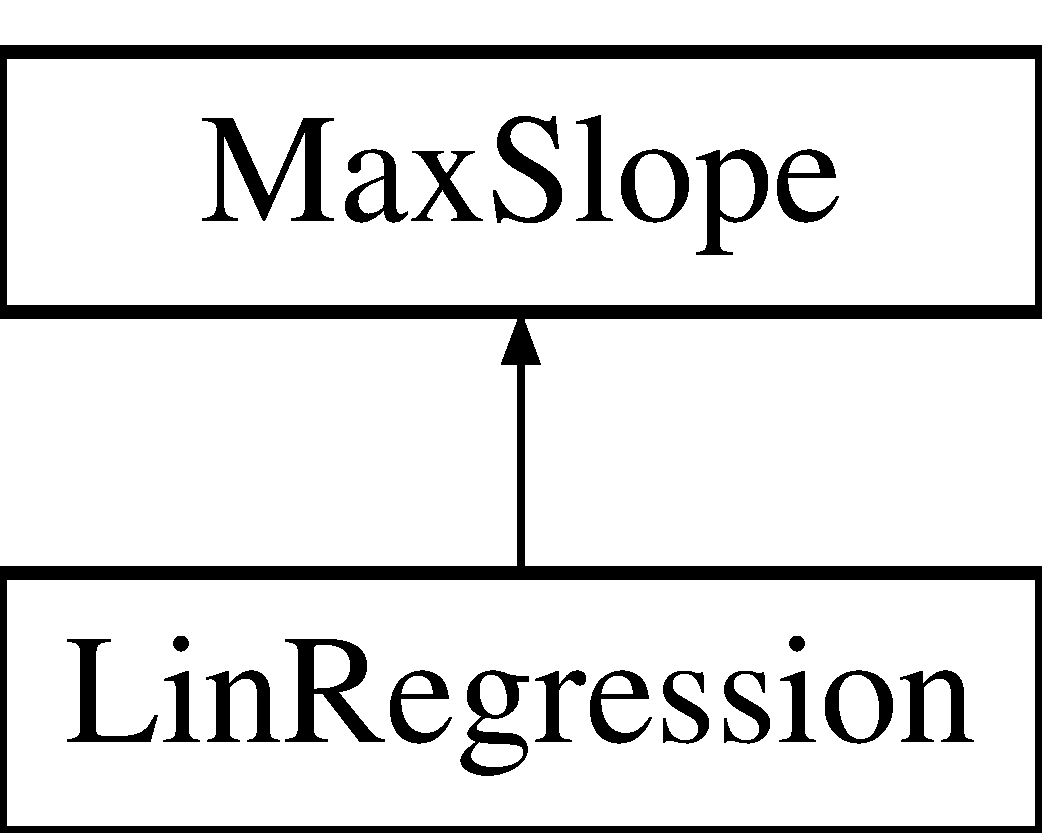
\includegraphics[height=2cm]{de/d89/classLinRegression}
\end{center}
\end{figure}
\subsection*{Public Member Functions}
\begin{DoxyCompactItemize}
\item 
\hyperlink{classLinRegression_a0d747e38f7a8997765be15f43062290c}{LinRegression} (const \hyperlink{classMatrix}{Matrix} \&progVar)
\begin{DoxyCompactList}\small\item\em Constructor. \item\end{DoxyCompactList}\item 
\hypertarget{classLinRegression_a4ea5ffb8032172bdf54d1f2d4041d520}{
\hyperlink{classLinRegression_a4ea5ffb8032172bdf54d1f2d4041d520}{$\sim$LinRegression} ()}
\label{de/d89/classLinRegression_a4ea5ffb8032172bdf54d1f2d4041d520}

\begin{DoxyCompactList}\small\item\em Destructor. \item\end{DoxyCompactList}\item 
int \hyperlink{classLinRegression_a1f245c4e47637f3f1d94f6129861406d}{MostMonotonic} (int $\ast$monoAry, const int ncols, const int col)
\begin{DoxyCompactList}\small\item\em Method to find the most monotonic progress variable. \item\end{DoxyCompactList}\end{DoxyCompactItemize}


\subsection{Constructor \& Destructor Documentation}
\hypertarget{classLinRegression_a0d747e38f7a8997765be15f43062290c}{
\index{LinRegression@{LinRegression}!LinRegression@{LinRegression}}
\index{LinRegression@{LinRegression}!LinRegression@{LinRegression}}
\subsubsection[{LinRegression}]{\setlength{\rightskip}{0pt plus 5cm}LinRegression::LinRegression (const {\bf Matrix} \& {\em progVar})}}
\label{de/d89/classLinRegression_a0d747e38f7a8997765be15f43062290c}


Constructor. 

\hyperlink{classLinRegression}{LinRegression} is a class that determines the most monotonic progress variable with respect to temperature (or another specified column). It calculates the slope of the best linear approximation for each progress variable and selects the largest magnitude.

The slope is given by \{sum\_\-i=1\_\-i=N (C\_\-i-\/C\_\-ave)(T\_\-i-\/T\_\-ave)\}/\{sum\_\-i=1\_\-i=N (T\_\-i-\/T\_\-ave)$^\wedge$2\} 

\subsection{Member Function Documentation}
\hypertarget{classLinRegression_a1f245c4e47637f3f1d94f6129861406d}{
\index{LinRegression@{LinRegression}!MostMonotonic@{MostMonotonic}}
\index{MostMonotonic@{MostMonotonic}!LinRegression@{LinRegression}}
\subsubsection[{MostMonotonic}]{\setlength{\rightskip}{0pt plus 5cm}int LinRegression::MostMonotonic (int $\ast$ {\em monoAry}, \/  const int {\em ncols}, \/  const int {\em col})\hspace{0.3cm}{\ttfamily  \mbox{[}virtual\mbox{]}}}}
\label{de/d89/classLinRegression_a1f245c4e47637f3f1d94f6129861406d}


Method to find the most monotonic progress variable. 

MostMonotonic calculates the slope of the best linear approximation for each progress variable which is strictly increasing or strictly decreasing. The output array monoAry must be of length ncols, where each cell holds a value of 3 if C is strictly monotonic and has the largest slope, 2 if C is strictly monotonic but does not have the largest slope, and 0 for non-\/monotonic C. col is the reference column. 

Implements \hyperlink{classMaxSlope_a494b1b1ae073d3b29fe7cdc023ce7861}{MaxSlope}.



The documentation for this class was generated from the following files:\begin{DoxyCompactItemize}
\item 
src/linregression.h\item 
src/linregression.cc\end{DoxyCompactItemize}

\hypertarget{classmatrix_1_1Matrix}{
\section{matrix::Matrix Class Reference}
\label{dd/db9/classmatrix_1_1Matrix}\index{matrix::Matrix@{matrix::Matrix}}
}
Inheritance diagram for matrix::Matrix:\begin{figure}[H]
\begin{center}
\leavevmode
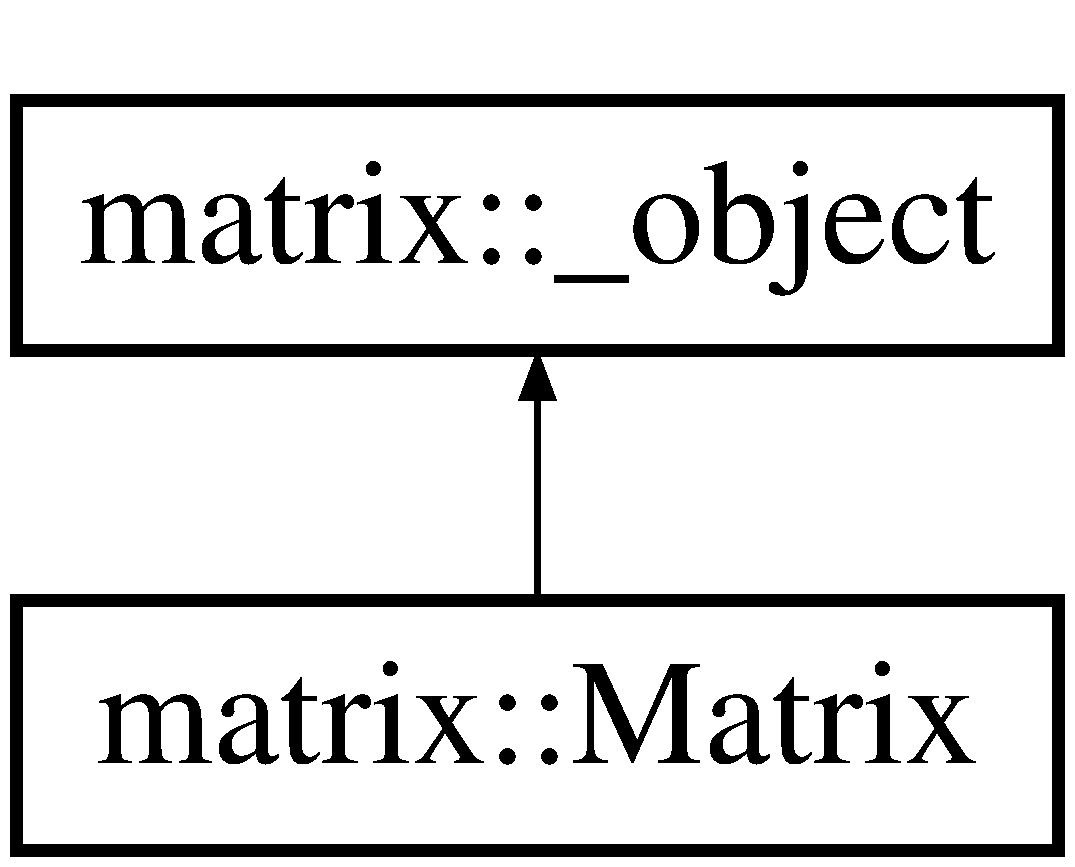
\includegraphics[height=2cm]{dd/db9/classmatrix_1_1Matrix}
\end{center}
\end{figure}
\subsection*{Public Member Functions}
\begin{DoxyCompactItemize}
\item 
\hypertarget{classmatrix_1_1Matrix_af668028ba2f2859741988054da60ee75}{
def {\bfseries \_\-\_\-init\_\-\_\-}}
\label{dd/db9/classmatrix_1_1Matrix_af668028ba2f2859741988054da60ee75}

\item 
\hypertarget{classmatrix_1_1Matrix_a78af2756e24b6f0d74695956b2f02646}{
def {\bfseries GetVal}}
\label{dd/db9/classmatrix_1_1Matrix_a78af2756e24b6f0d74695956b2f02646}

\item 
\hypertarget{classmatrix_1_1Matrix_ae7b5ee268f12fb34ebbbe7213f91638a}{
def {\bfseries SetVal}}
\label{dd/db9/classmatrix_1_1Matrix_ae7b5ee268f12fb34ebbbe7213f91638a}

\item 
\hypertarget{classmatrix_1_1Matrix_a25ad06ac9533ca524f9f17734d6a1ad6}{
def {\bfseries GetNumRows}}
\label{dd/db9/classmatrix_1_1Matrix_a25ad06ac9533ca524f9f17734d6a1ad6}

\item 
\hypertarget{classmatrix_1_1Matrix_af4ec3fb39dcbec6b92df554051019e6d}{
def {\bfseries GetNumCols}}
\label{dd/db9/classmatrix_1_1Matrix_af4ec3fb39dcbec6b92df554051019e6d}

\item 
\hypertarget{classmatrix_1_1Matrix_a81fd68a34b15d0f2412818b39eaaf02c}{
def {\bfseries GetCol}}
\label{dd/db9/classmatrix_1_1Matrix_a81fd68a34b15d0f2412818b39eaaf02c}

\end{DoxyCompactItemize}
\subsection*{Public Attributes}
\begin{DoxyCompactItemize}
\item 
\hypertarget{classmatrix_1_1Matrix_acc21534927e527008524f070e1a8f5fd}{
{\bfseries this}}
\label{dd/db9/classmatrix_1_1Matrix_acc21534927e527008524f070e1a8f5fd}

\end{DoxyCompactItemize}


The documentation for this class was generated from the following file:\begin{DoxyCompactItemize}
\item 
src/matrix.py\end{DoxyCompactItemize}

\hypertarget{classMatrix}{
\section{Matrix Class Reference}
\label{d3/d3f/classMatrix}\index{Matrix@{Matrix}}
}
\subsection*{Public Member Functions}
\begin{DoxyCompactItemize}
\item 
\hypertarget{classMatrix_a7213414e405fd1c81c394d5053721fa7}{
\hyperlink{classMatrix_a7213414e405fd1c81c394d5053721fa7}{Matrix} (int rows, int cols)}
\label{d3/d3f/classMatrix_a7213414e405fd1c81c394d5053721fa7}

\begin{DoxyCompactList}\small\item\em Constructor. \item\end{DoxyCompactList}\item 
\hypertarget{classMatrix_a9b1c3627f573d78a2f08623fdfef990f}{
\hyperlink{classMatrix_a9b1c3627f573d78a2f08623fdfef990f}{$\sim$Matrix} ()}
\label{d3/d3f/classMatrix_a9b1c3627f573d78a2f08623fdfef990f}

\begin{DoxyCompactList}\small\item\em Destructor. \item\end{DoxyCompactList}\item 
\hypertarget{classMatrix_ad7da71a311eeedf1ac24be5c6ada4dcb}{
double \hyperlink{classMatrix_ad7da71a311eeedf1ac24be5c6ada4dcb}{GetVal} (int i, int j) const }
\label{d3/d3f/classMatrix_ad7da71a311eeedf1ac24be5c6ada4dcb}

\begin{DoxyCompactList}\small\item\em Get the value at a specified index. \item\end{DoxyCompactList}\item 
\hypertarget{classMatrix_aa8c1c4e96ce2dff650a31dd0650db7db}{
void \hyperlink{classMatrix_aa8c1c4e96ce2dff650a31dd0650db7db}{SetVal} (int i, int j, double val)}
\label{d3/d3f/classMatrix_aa8c1c4e96ce2dff650a31dd0650db7db}

\begin{DoxyCompactList}\small\item\em Set the value at a specific location. \item\end{DoxyCompactList}\item 
\hypertarget{classMatrix_ae683a43cfb2cb84e8f6fa0297744b307}{
int \hyperlink{classMatrix_ae683a43cfb2cb84e8f6fa0297744b307}{GetNumRows} () const }
\label{d3/d3f/classMatrix_ae683a43cfb2cb84e8f6fa0297744b307}

\begin{DoxyCompactList}\small\item\em Return the number of rows. \item\end{DoxyCompactList}\item 
\hypertarget{classMatrix_a4069e97fcef57fce6828c6042d63e7d2}{
int \hyperlink{classMatrix_a4069e97fcef57fce6828c6042d63e7d2}{GetNumCols} () const }
\label{d3/d3f/classMatrix_a4069e97fcef57fce6828c6042d63e7d2}

\begin{DoxyCompactList}\small\item\em Return the number of columns. \item\end{DoxyCompactList}\item 
\hypertarget{classMatrix_a830c8a78828c4db552648e46aef5ec6e}{
int \hyperlink{classMatrix_a830c8a78828c4db552648e46aef5ec6e}{GetCol} (int j, double $\ast$colAry) const }
\label{d3/d3f/classMatrix_a830c8a78828c4db552648e46aef5ec6e}

\begin{DoxyCompactList}\small\item\em Return an array containing column j. \item\end{DoxyCompactList}\end{DoxyCompactItemize}


The documentation for this class was generated from the following files:\begin{DoxyCompactItemize}
\item 
src/matrix.h\item 
src/matrix.cc\end{DoxyCompactItemize}

\hypertarget{classmonocheck_1_1Matrix}{
\section{monocheck::Matrix Class Reference}
\label{d3/d15/classmonocheck_1_1Matrix}\index{monocheck::Matrix@{monocheck::Matrix}}
}
Inheritance diagram for monocheck::Matrix:\begin{figure}[H]
\begin{center}
\leavevmode
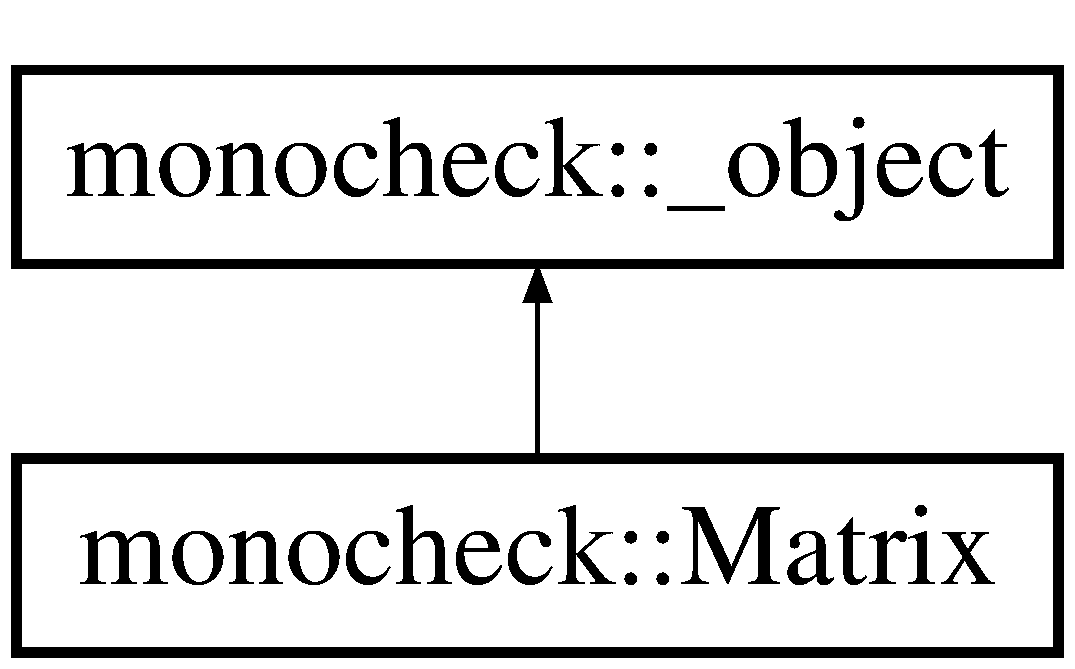
\includegraphics[height=2cm]{d3/d15/classmonocheck_1_1Matrix}
\end{center}
\end{figure}
\subsection*{Public Member Functions}
\begin{DoxyCompactItemize}
\item 
\hypertarget{classmonocheck_1_1Matrix_a24536d0f43c78981935dd94967a121cf}{
def {\bfseries \_\-\_\-init\_\-\_\-}}
\label{d3/d15/classmonocheck_1_1Matrix_a24536d0f43c78981935dd94967a121cf}

\item 
\hypertarget{classmonocheck_1_1Matrix_aa3a58278b48efcfff8e5c491b7f86b44}{
def {\bfseries GetVal}}
\label{d3/d15/classmonocheck_1_1Matrix_aa3a58278b48efcfff8e5c491b7f86b44}

\item 
\hypertarget{classmonocheck_1_1Matrix_ac3c442daf925b657fe290c72dae1271c}{
def {\bfseries SetVal}}
\label{d3/d15/classmonocheck_1_1Matrix_ac3c442daf925b657fe290c72dae1271c}

\item 
\hypertarget{classmonocheck_1_1Matrix_abdb690f5b480564be56ff839f6cd79e7}{
def {\bfseries GetNumRows}}
\label{d3/d15/classmonocheck_1_1Matrix_abdb690f5b480564be56ff839f6cd79e7}

\item 
\hypertarget{classmonocheck_1_1Matrix_afe4ec68e3ecf301292b417cc2daf1db3}{
def {\bfseries GetNumCols}}
\label{d3/d15/classmonocheck_1_1Matrix_afe4ec68e3ecf301292b417cc2daf1db3}

\item 
\hypertarget{classmonocheck_1_1Matrix_af023859e735f04776b64d225d58ec5a5}{
def {\bfseries GetCol}}
\label{d3/d15/classmonocheck_1_1Matrix_af023859e735f04776b64d225d58ec5a5}

\end{DoxyCompactItemize}
\subsection*{Public Attributes}
\begin{DoxyCompactItemize}
\item 
\hypertarget{classmonocheck_1_1Matrix_aaa81a06876b224d4caf8663c14444835}{
{\bfseries this}}
\label{d3/d15/classmonocheck_1_1Matrix_aaa81a06876b224d4caf8663c14444835}

\end{DoxyCompactItemize}


The documentation for this class was generated from the following file:\begin{DoxyCompactItemize}
\item 
src/monocheck.py\end{DoxyCompactItemize}

\hypertarget{classMatrix3D}{
\section{Matrix3D Class Reference}
\label{d0/dcb/classMatrix3D}\index{Matrix3D@{Matrix3D}}
}
\subsection*{Public Member Functions}
\begin{DoxyCompactItemize}
\item 
\hypertarget{classMatrix3D_a79ffea45e6ad9f5789f5444f033cb8f4}{
\hyperlink{classMatrix3D_a79ffea45e6ad9f5789f5444f033cb8f4}{Matrix3D} (int dim1, int dim2, int dim3)}
\label{d0/dcb/classMatrix3D_a79ffea45e6ad9f5789f5444f033cb8f4}

\begin{DoxyCompactList}\small\item\em Constructor. \item\end{DoxyCompactList}\item 
\hypertarget{classMatrix3D_a67ebf80ff62e71d327066491811401af}{
\hyperlink{classMatrix3D_a67ebf80ff62e71d327066491811401af}{$\sim$Matrix3D} ()}
\label{d0/dcb/classMatrix3D_a67ebf80ff62e71d327066491811401af}

\begin{DoxyCompactList}\small\item\em Destructor. \item\end{DoxyCompactList}\item 
\hypertarget{classMatrix3D_a8422daf16b13a3a26f3856dcadfae291}{
double \hyperlink{classMatrix3D_a8422daf16b13a3a26f3856dcadfae291}{GetVal} (int i, int j, int k) const }
\label{d0/dcb/classMatrix3D_a8422daf16b13a3a26f3856dcadfae291}

\begin{DoxyCompactList}\small\item\em Get the value at a specified index. \item\end{DoxyCompactList}\item 
\hypertarget{classMatrix3D_a082378ce9c6565d0655cb0ec2e68116c}{
void \hyperlink{classMatrix3D_a082378ce9c6565d0655cb0ec2e68116c}{SetVal} (int i, int j, int k, double vol)}
\label{d0/dcb/classMatrix3D_a082378ce9c6565d0655cb0ec2e68116c}

\begin{DoxyCompactList}\small\item\em Set the value at a specified index. \item\end{DoxyCompactList}\item 
\hypertarget{classMatrix3D_a97e904be2b5177157d7ecb11488c6ef3}{
int \hyperlink{classMatrix3D_a97e904be2b5177157d7ecb11488c6ef3}{GetNumDim1} () const }
\label{d0/dcb/classMatrix3D_a97e904be2b5177157d7ecb11488c6ef3}

\begin{DoxyCompactList}\small\item\em Return dim1. \item\end{DoxyCompactList}\item 
\hypertarget{classMatrix3D_ad6895586f9041457377a2b4e0b5778ce}{
int \hyperlink{classMatrix3D_ad6895586f9041457377a2b4e0b5778ce}{GetNumDim2} () const }
\label{d0/dcb/classMatrix3D_ad6895586f9041457377a2b4e0b5778ce}

\begin{DoxyCompactList}\small\item\em Return dim2. \item\end{DoxyCompactList}\item 
\hypertarget{classMatrix3D_aa98e87c6887afa3141cd290818650932}{
int \hyperlink{classMatrix3D_aa98e87c6887afa3141cd290818650932}{GetNumDim3} () const }
\label{d0/dcb/classMatrix3D_aa98e87c6887afa3141cd290818650932}

\begin{DoxyCompactList}\small\item\em Return dim3. \item\end{DoxyCompactList}\end{DoxyCompactItemize}


The documentation for this class was generated from the following files:\begin{DoxyCompactItemize}
\item 
src/matrix3d.h\item 
src/matrix3d.cc\end{DoxyCompactItemize}

\hypertarget{classmatrix3d_1_1Matrix3D}{
\section{matrix3d::Matrix3D Class Reference}
\label{d4/dbb/classmatrix3d_1_1Matrix3D}\index{matrix3d::Matrix3D@{matrix3d::Matrix3D}}
}
Inheritance diagram for matrix3d::Matrix3D:\begin{figure}[H]
\begin{center}
\leavevmode
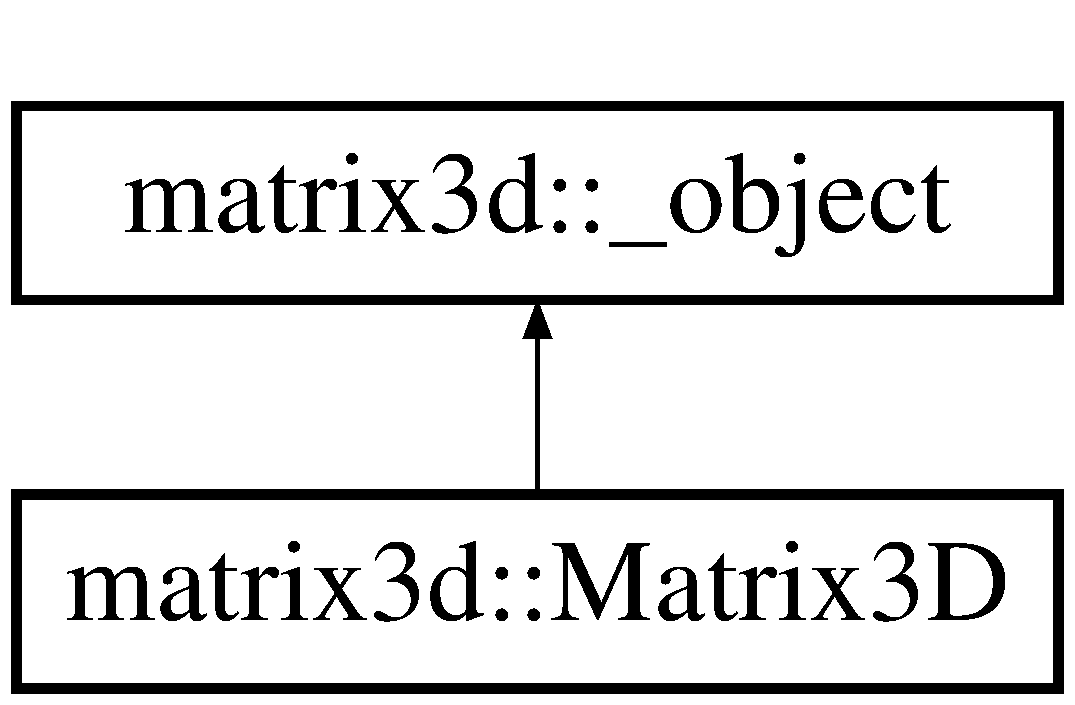
\includegraphics[height=2cm]{d4/dbb/classmatrix3d_1_1Matrix3D}
\end{center}
\end{figure}
\subsection*{Public Member Functions}
\begin{DoxyCompactItemize}
\item 
\hypertarget{classmatrix3d_1_1Matrix3D_afc828ef75c2d6fda473bab6673006fc2}{
def {\bfseries \_\-\_\-init\_\-\_\-}}
\label{d4/dbb/classmatrix3d_1_1Matrix3D_afc828ef75c2d6fda473bab6673006fc2}

\item 
\hypertarget{classmatrix3d_1_1Matrix3D_a9647e57d80350d7910056de98e6bfc2a}{
def {\bfseries GetVal}}
\label{d4/dbb/classmatrix3d_1_1Matrix3D_a9647e57d80350d7910056de98e6bfc2a}

\item 
\hypertarget{classmatrix3d_1_1Matrix3D_a1996596a1f5a693c6f8e320aef7b7710}{
def {\bfseries SetVal}}
\label{d4/dbb/classmatrix3d_1_1Matrix3D_a1996596a1f5a693c6f8e320aef7b7710}

\item 
\hypertarget{classmatrix3d_1_1Matrix3D_a6b2c6828d4b23fac9e5d73947cd8fd5c}{
def {\bfseries GetNumDim1}}
\label{d4/dbb/classmatrix3d_1_1Matrix3D_a6b2c6828d4b23fac9e5d73947cd8fd5c}

\item 
\hypertarget{classmatrix3d_1_1Matrix3D_a11ba8f2b438f400343f199d3eb858714}{
def {\bfseries GetNumDim2}}
\label{d4/dbb/classmatrix3d_1_1Matrix3D_a11ba8f2b438f400343f199d3eb858714}

\item 
\hypertarget{classmatrix3d_1_1Matrix3D_a23d415fad6978cae908870e45ebc30cc}{
def {\bfseries GetNumDim3}}
\label{d4/dbb/classmatrix3d_1_1Matrix3D_a23d415fad6978cae908870e45ebc30cc}

\end{DoxyCompactItemize}
\subsection*{Public Attributes}
\begin{DoxyCompactItemize}
\item 
\hypertarget{classmatrix3d_1_1Matrix3D_adb19e1ac1341d747d9f7a9e70e89f053}{
{\bfseries this}}
\label{d4/dbb/classmatrix3d_1_1Matrix3D_adb19e1ac1341d747d9f7a9e70e89f053}

\end{DoxyCompactItemize}


The documentation for this class was generated from the following file:\begin{DoxyCompactItemize}
\item 
src/matrix3d.py\end{DoxyCompactItemize}

\hypertarget{classMatrix4D}{
\section{Matrix4D Class Reference}
\label{d7/d9c/classMatrix4D}\index{Matrix4D@{Matrix4D}}
}
\subsection*{Public Member Functions}
\begin{DoxyCompactItemize}
\item 
\hypertarget{classMatrix4D_ac4ef4cb38ec681c8ae057081aa1235ef}{
\hyperlink{classMatrix4D_ac4ef4cb38ec681c8ae057081aa1235ef}{Matrix4D} (int dim1, int dim2, int dim3, int dim4)}
\label{d7/d9c/classMatrix4D_ac4ef4cb38ec681c8ae057081aa1235ef}

\begin{DoxyCompactList}\small\item\em Constructor. \item\end{DoxyCompactList}\item 
\hypertarget{classMatrix4D_a90b64981f087dfcb496b8f5a0449803c}{
\hyperlink{classMatrix4D_a90b64981f087dfcb496b8f5a0449803c}{$\sim$Matrix4D} ()}
\label{d7/d9c/classMatrix4D_a90b64981f087dfcb496b8f5a0449803c}

\begin{DoxyCompactList}\small\item\em Destructor. \item\end{DoxyCompactList}\item 
\hypertarget{classMatrix4D_a03f55155ae67a6741a662494ac7da18a}{
double \hyperlink{classMatrix4D_a03f55155ae67a6741a662494ac7da18a}{GetVal} (int i, int j, int k, int l) const }
\label{d7/d9c/classMatrix4D_a03f55155ae67a6741a662494ac7da18a}

\begin{DoxyCompactList}\small\item\em Get the value at a specified index. \item\end{DoxyCompactList}\item 
\hypertarget{classMatrix4D_a113ab746b94d6c253823f53cae3b8181}{
void \hyperlink{classMatrix4D_a113ab746b94d6c253823f53cae3b8181}{SetVal} (int i, int j, int k, int l, double val)}
\label{d7/d9c/classMatrix4D_a113ab746b94d6c253823f53cae3b8181}

\begin{DoxyCompactList}\small\item\em Set the value at a specified index. \item\end{DoxyCompactList}\item 
\hypertarget{classMatrix4D_a7582cae941bf64578b9099ad91afc869}{
int \hyperlink{classMatrix4D_a7582cae941bf64578b9099ad91afc869}{GetNumDim1} () const }
\label{d7/d9c/classMatrix4D_a7582cae941bf64578b9099ad91afc869}

\begin{DoxyCompactList}\small\item\em Return dim1. \item\end{DoxyCompactList}\item 
\hypertarget{classMatrix4D_a911bf63762bff343b18402a6c1dd9345}{
int \hyperlink{classMatrix4D_a911bf63762bff343b18402a6c1dd9345}{GetNumDim2} () const }
\label{d7/d9c/classMatrix4D_a911bf63762bff343b18402a6c1dd9345}

\begin{DoxyCompactList}\small\item\em Return dim2. \item\end{DoxyCompactList}\item 
\hypertarget{classMatrix4D_a65fcee9bc1c4eff1210799cf5d72bbe2}{
int \hyperlink{classMatrix4D_a65fcee9bc1c4eff1210799cf5d72bbe2}{GetNumDim3} () const }
\label{d7/d9c/classMatrix4D_a65fcee9bc1c4eff1210799cf5d72bbe2}

\begin{DoxyCompactList}\small\item\em Return dim3. \item\end{DoxyCompactList}\item 
\hypertarget{classMatrix4D_abf9f0c77981cd832b6baaf2c934d92ef}{
int \hyperlink{classMatrix4D_abf9f0c77981cd832b6baaf2c934d92ef}{GetNumDim4} () const }
\label{d7/d9c/classMatrix4D_abf9f0c77981cd832b6baaf2c934d92ef}

\begin{DoxyCompactList}\small\item\em Return dim4. \item\end{DoxyCompactList}\end{DoxyCompactItemize}


The documentation for this class was generated from the following files:\begin{DoxyCompactItemize}
\item 
src/matrix4d.h\item 
src/matrix4d.cc\end{DoxyCompactItemize}

\hypertarget{classmatrix4d_1_1Matrix4D}{
\section{matrix4d::Matrix4D Class Reference}
\label{d8/d2d/classmatrix4d_1_1Matrix4D}\index{matrix4d::Matrix4D@{matrix4d::Matrix4D}}
}
Inheritance diagram for matrix4d::Matrix4D:\begin{figure}[H]
\begin{center}
\leavevmode
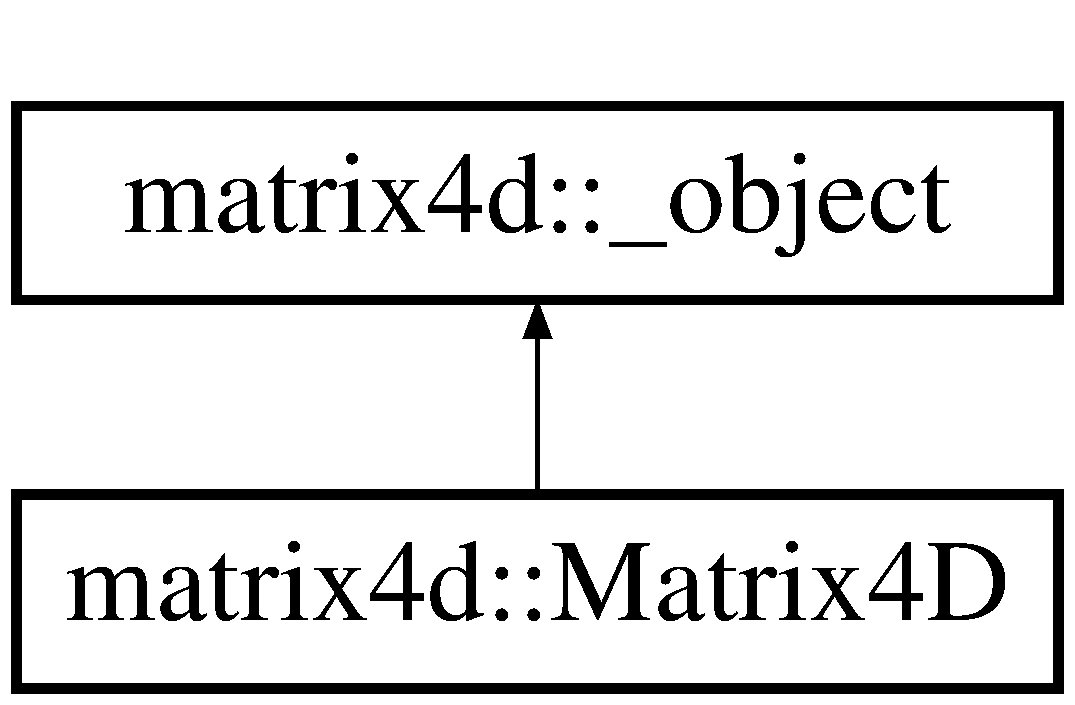
\includegraphics[height=2cm]{d8/d2d/classmatrix4d_1_1Matrix4D}
\end{center}
\end{figure}
\subsection*{Public Member Functions}
\begin{DoxyCompactItemize}
\item 
\hypertarget{classmatrix4d_1_1Matrix4D_aa8d774229c413810f9b45e3f9639e14a}{
def {\bfseries \_\-\_\-init\_\-\_\-}}
\label{d8/d2d/classmatrix4d_1_1Matrix4D_aa8d774229c413810f9b45e3f9639e14a}

\item 
\hypertarget{classmatrix4d_1_1Matrix4D_a6fafbf238ef7c28349d531f83fd8cf33}{
def {\bfseries GetVal}}
\label{d8/d2d/classmatrix4d_1_1Matrix4D_a6fafbf238ef7c28349d531f83fd8cf33}

\item 
\hypertarget{classmatrix4d_1_1Matrix4D_a2b5889d9f828b99718de148fca1be9f9}{
def {\bfseries SetVal}}
\label{d8/d2d/classmatrix4d_1_1Matrix4D_a2b5889d9f828b99718de148fca1be9f9}

\item 
\hypertarget{classmatrix4d_1_1Matrix4D_a3f9d959c9d4c8d5320747d7ee04c9fec}{
def {\bfseries GetNumDim1}}
\label{d8/d2d/classmatrix4d_1_1Matrix4D_a3f9d959c9d4c8d5320747d7ee04c9fec}

\item 
\hypertarget{classmatrix4d_1_1Matrix4D_a95aa43f9651d99efa51c414cbde29838}{
def {\bfseries GetNumDim2}}
\label{d8/d2d/classmatrix4d_1_1Matrix4D_a95aa43f9651d99efa51c414cbde29838}

\item 
\hypertarget{classmatrix4d_1_1Matrix4D_af60a9f91fa2c528f76bea466db63dd12}{
def {\bfseries GetNumDim3}}
\label{d8/d2d/classmatrix4d_1_1Matrix4D_af60a9f91fa2c528f76bea466db63dd12}

\item 
\hypertarget{classmatrix4d_1_1Matrix4D_ad1da489a0f84e1092e77a7586c03a062}{
def {\bfseries GetNumDim4}}
\label{d8/d2d/classmatrix4d_1_1Matrix4D_ad1da489a0f84e1092e77a7586c03a062}

\end{DoxyCompactItemize}
\subsection*{Public Attributes}
\begin{DoxyCompactItemize}
\item 
\hypertarget{classmatrix4d_1_1Matrix4D_a874437e826daf81e59bd8dad0fb64f00}{
{\bfseries this}}
\label{d8/d2d/classmatrix4d_1_1Matrix4D_a874437e826daf81e59bd8dad0fb64f00}

\end{DoxyCompactItemize}


The documentation for this class was generated from the following file:\begin{DoxyCompactItemize}
\item 
src/matrix4d.py\end{DoxyCompactItemize}

\hypertarget{classmaxslope_1_1MaxSlope}{
\section{maxslope::MaxSlope Class Reference}
\label{d8/deb/classmaxslope_1_1MaxSlope}\index{maxslope::MaxSlope@{maxslope::MaxSlope}}
}
Inheritance diagram for maxslope::MaxSlope:\begin{figure}[H]
\begin{center}
\leavevmode
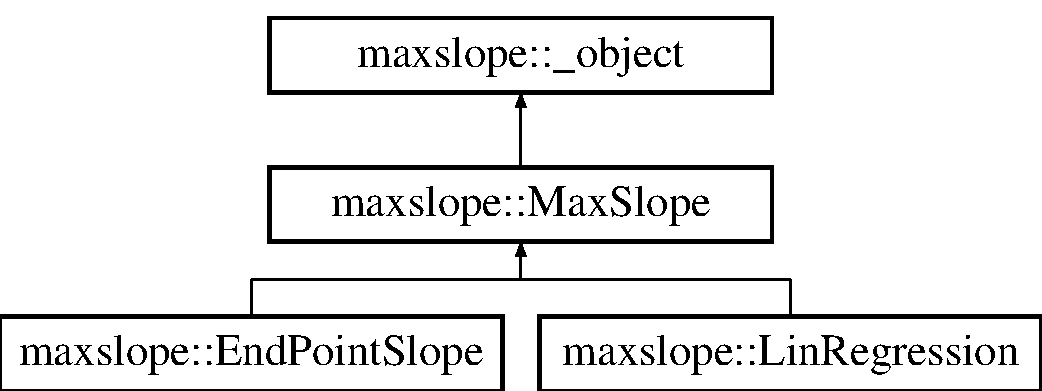
\includegraphics[height=3cm]{d8/deb/classmaxslope_1_1MaxSlope}
\end{center}
\end{figure}
\subsection*{Public Member Functions}
\begin{DoxyCompactItemize}
\item 
\hypertarget{classmaxslope_1_1MaxSlope_a362903e9e198c5d097c7c09ae6f74dd8}{
def {\bfseries \_\-\_\-init\_\-\_\-}}
\label{d8/deb/classmaxslope_1_1MaxSlope_a362903e9e198c5d097c7c09ae6f74dd8}

\item 
\hypertarget{classmaxslope_1_1MaxSlope_a6fda530ba01a2b4bc78f7c1ad841cabf}{
def {\bfseries MostMonotonic}}
\label{d8/deb/classmaxslope_1_1MaxSlope_a6fda530ba01a2b4bc78f7c1ad841cabf}

\end{DoxyCompactItemize}


The documentation for this class was generated from the following file:\begin{DoxyCompactItemize}
\item 
src/maxslope.py\end{DoxyCompactItemize}

\hypertarget{classMaxSlope}{
\section{MaxSlope Class Reference}
\label{d0/d39/classMaxSlope}\index{MaxSlope@{MaxSlope}}
}
Inheritance diagram for MaxSlope:\begin{figure}[H]
\begin{center}
\leavevmode
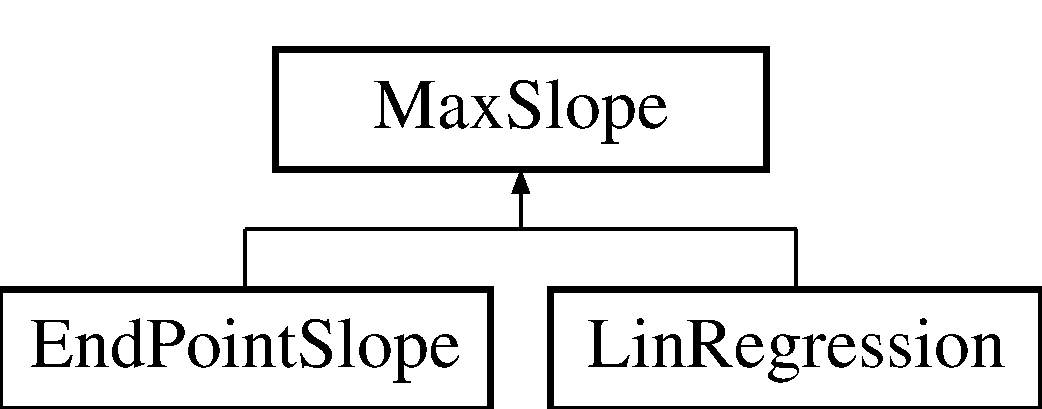
\includegraphics[height=2cm]{d0/d39/classMaxSlope}
\end{center}
\end{figure}
\subsection*{Public Member Functions}
\begin{DoxyCompactItemize}
\item 
\hypertarget{classMaxSlope_a494b1b1ae073d3b29fe7cdc023ce7861}{
virtual int \hyperlink{classMaxSlope_a494b1b1ae073d3b29fe7cdc023ce7861}{MostMonotonic} (int $\ast$monoAry, const int ncols, const int col)=0}
\label{d0/d39/classMaxSlope_a494b1b1ae073d3b29fe7cdc023ce7861}

\begin{DoxyCompactList}\small\item\em Virtual function to be inherited by each monotonicity checking algorithm to determine the most monotonic progress variable. \item\end{DoxyCompactList}\end{DoxyCompactItemize}


The documentation for this class was generated from the following file:\begin{DoxyCompactItemize}
\item 
src/maxslope.h\end{DoxyCompactItemize}

\hypertarget{classMonoCheck}{
\section{MonoCheck Class Reference}
\label{d8/ddf/classMonoCheck}\index{MonoCheck@{MonoCheck}}
}
\subsection*{Public Member Functions}
\begin{DoxyCompactItemize}
\item 
\hyperlink{classMonoCheck_a4cee9c89dd8a6c19cd01d597343c4d99}{MonoCheck} (const \hyperlink{classMatrix}{Matrix} \&progVar)
\begin{DoxyCompactList}\small\item\em Constructor. \item\end{DoxyCompactList}\item 
\hypertarget{classMonoCheck_a97dc563e5cad68eafabd498d66e86590}{
\hyperlink{classMonoCheck_a97dc563e5cad68eafabd498d66e86590}{$\sim$MonoCheck} ()}
\label{d8/ddf/classMonoCheck_a97dc563e5cad68eafabd498d66e86590}

\begin{DoxyCompactList}\small\item\em Destructor. \item\end{DoxyCompactList}\item 
int \hyperlink{classMonoCheck_af34f3d72ec2d1575526d42bfe4cdfe7a}{CheckStrictMonoticity} (int $\ast$monoAry, const int ncols, int col)
\begin{DoxyCompactList}\small\item\em Method to check whether each progress variable is strictly monotonic. \item\end{DoxyCompactList}\end{DoxyCompactItemize}


\subsection{Constructor \& Destructor Documentation}
\hypertarget{classMonoCheck_a4cee9c89dd8a6c19cd01d597343c4d99}{
\index{MonoCheck@{MonoCheck}!MonoCheck@{MonoCheck}}
\index{MonoCheck@{MonoCheck}!MonoCheck@{MonoCheck}}
\subsubsection[{MonoCheck}]{\setlength{\rightskip}{0pt plus 5cm}MonoCheck::MonoCheck (const {\bf Matrix} \& {\em progVar})}}
\label{d8/ddf/classMonoCheck_a4cee9c89dd8a6c19cd01d597343c4d99}


Constructor. 

monocheck is a class which checks whether a specified progress variable is strictly increasing or strictly decreasing with respect to temperature (or another specified column). That is, C(T1)$<$C(T2) or C(T1)$>$C(T2) for T1$<$T2, where T1 and T2 are any two temperatures and C is the progress variable. 

\subsection{Member Function Documentation}
\hypertarget{classMonoCheck_af34f3d72ec2d1575526d42bfe4cdfe7a}{
\index{MonoCheck@{MonoCheck}!CheckStrictMonoticity@{CheckStrictMonoticity}}
\index{CheckStrictMonoticity@{CheckStrictMonoticity}!MonoCheck@{MonoCheck}}
\subsubsection[{CheckStrictMonoticity}]{\setlength{\rightskip}{0pt plus 5cm}int MonoCheck::CheckStrictMonoticity (int $\ast$ {\em monoAry}, \/  const int {\em ncols}, \/  int {\em col})}}
\label{d8/ddf/classMonoCheck_af34f3d72ec2d1575526d42bfe4cdfe7a}


Method to check whether each progress variable is strictly monotonic. 

CheckStrictMonoticity checks the monotonicity of each column (AKA progress variable \char`\"{}C\char`\"{}) in progVar with respect to column \char`\"{}col\char`\"{}. The output array monoAry must be of length ncols\_\-, where each cell holds a value of 3 if C is strictly increasing or strictly decreasing and 0 otherwise.

\begin{DoxyVerb}
INPUTS:

int *monoAry        array containing integer flags that denote the monotonicity of candidate progress variables

const int ncols     number of columns of monoAry

const int col       the reference column


OUTPUT:

int                 flag specifying whether or not the function succeeded
                     = 0: success
		    != 0: something went wrong

\end{DoxyVerb}
 

The documentation for this class was generated from the following files:\begin{DoxyCompactItemize}
\item 
src/monocheck.h\item 
src/monocheck.cc\end{DoxyCompactItemize}

\hypertarget{classmonocheck_1_1MonoCheck}{
\section{monocheck::MonoCheck Class Reference}
\label{d7/de1/classmonocheck_1_1MonoCheck}\index{monocheck::MonoCheck@{monocheck::MonoCheck}}
}
Inheritance diagram for monocheck::MonoCheck:\begin{figure}[H]
\begin{center}
\leavevmode
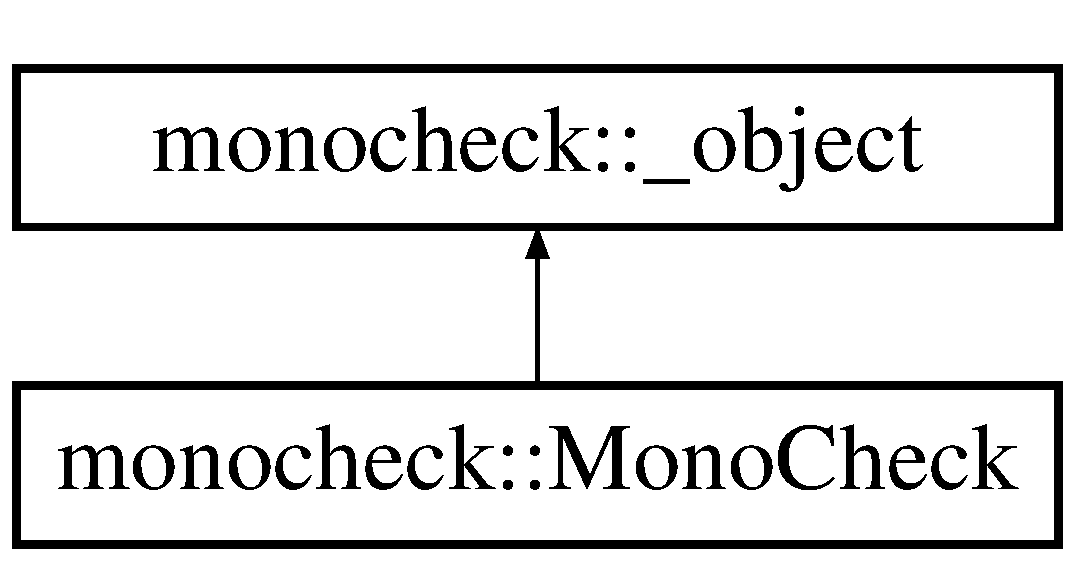
\includegraphics[height=2cm]{d7/de1/classmonocheck_1_1MonoCheck}
\end{center}
\end{figure}
\subsection*{Public Member Functions}
\begin{DoxyCompactItemize}
\item 
\hypertarget{classmonocheck_1_1MonoCheck_a69a5e0b89b39ff0c0caac2604605dddd}{
def {\bfseries \_\-\_\-init\_\-\_\-}}
\label{d7/de1/classmonocheck_1_1MonoCheck_a69a5e0b89b39ff0c0caac2604605dddd}

\item 
\hypertarget{classmonocheck_1_1MonoCheck_a9684b1459e63268cf3a3962e79827355}{
def {\bfseries CheckStrictMonoticity}}
\label{d7/de1/classmonocheck_1_1MonoCheck_a9684b1459e63268cf3a3962e79827355}

\end{DoxyCompactItemize}
\subsection*{Public Attributes}
\begin{DoxyCompactItemize}
\item 
\hypertarget{classmonocheck_1_1MonoCheck_a4e896031c1c1933907b882f4c4807cae}{
{\bfseries this}}
\label{d7/de1/classmonocheck_1_1MonoCheck_a4e896031c1c1933907b882f4c4807cae}

\end{DoxyCompactItemize}


The documentation for this class was generated from the following file:\begin{DoxyCompactItemize}
\item 
src/monocheck.py\end{DoxyCompactItemize}

\hypertarget{classPDF}{
\section{PDF Class Reference}
\label{dc/d2d/classPDF}\index{PDF@{PDF}}
}
Inheritance diagram for PDF:\begin{figure}[H]
\begin{center}
\leavevmode
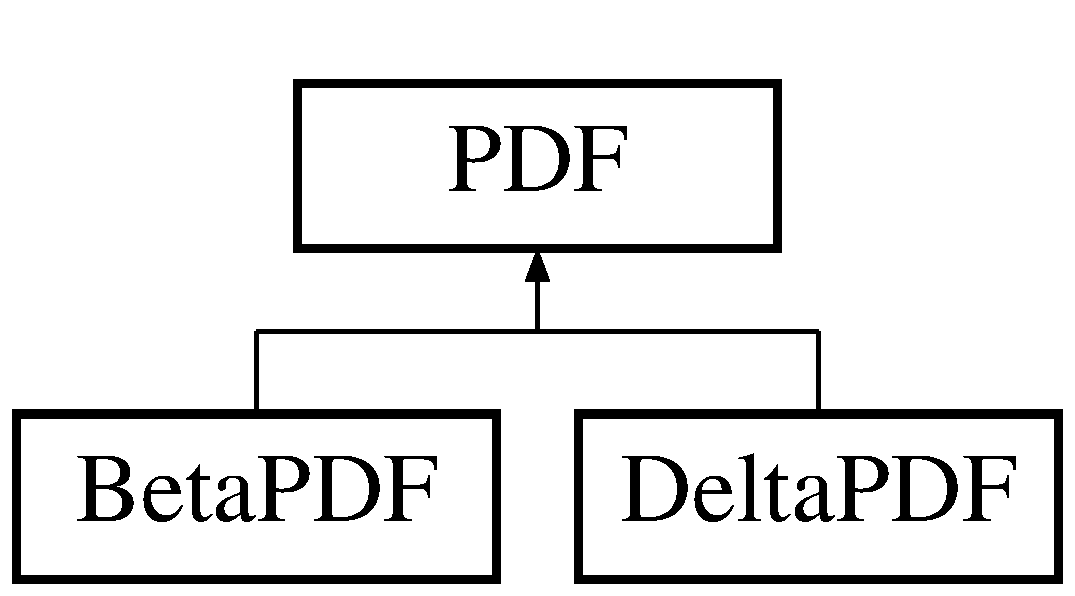
\includegraphics[height=2cm]{dc/d2d/classPDF}
\end{center}
\end{figure}
\subsection*{Public Member Functions}
\begin{DoxyCompactItemize}
\item 
\hypertarget{classPDF_aa1c76d504f181d271734bba54068c51b}{
virtual int {\bfseries pdfVal} (const double $\ast$Z, const int ZPoints, \hyperlink{classMatrix3D}{Matrix3D} $\ast$pdfValM)=0}
\label{dc/d2d/classPDF_aa1c76d504f181d271734bba54068c51b}

\end{DoxyCompactItemize}


The documentation for this class was generated from the following file:\begin{DoxyCompactItemize}
\item 
src/pdf.h\end{DoxyCompactItemize}

\hypertarget{classpdf_1_1PDF}{
\section{pdf::PDF Class Reference}
\label{dd/d66/classpdf_1_1PDF}\index{pdf::PDF@{pdf::PDF}}
}
Inheritance diagram for pdf::PDF:\begin{figure}[H]
\begin{center}
\leavevmode
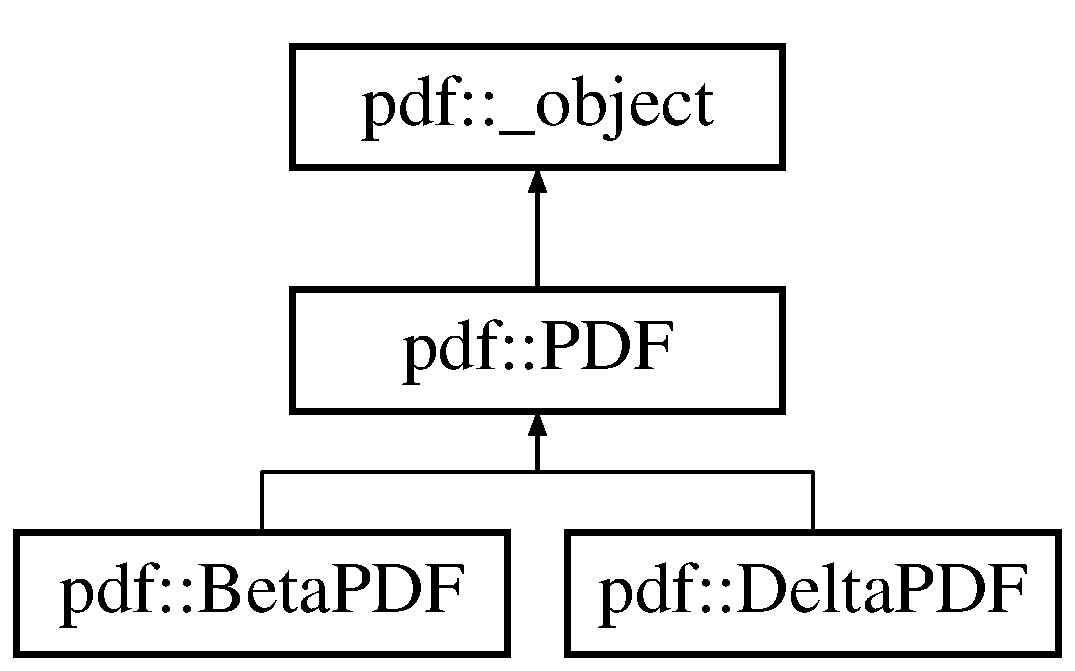
\includegraphics[height=3cm]{dd/d66/classpdf_1_1PDF}
\end{center}
\end{figure}
\subsection*{Public Member Functions}
\begin{DoxyCompactItemize}
\item 
\hypertarget{classpdf_1_1PDF_ad3afb94bbbcb72475c89d7bb3f946da2}{
def {\bfseries \_\-\_\-init\_\-\_\-}}
\label{dd/d66/classpdf_1_1PDF_ad3afb94bbbcb72475c89d7bb3f946da2}

\item 
\hypertarget{classpdf_1_1PDF_a44e17a10e5b431ab10ed1f5741d05e30}{
def {\bfseries pdfVal}}
\label{dd/d66/classpdf_1_1PDF_a44e17a10e5b431ab10ed1f5741d05e30}

\end{DoxyCompactItemize}


The documentation for this class was generated from the following file:\begin{DoxyCompactItemize}
\item 
src/pdf.py\end{DoxyCompactItemize}

\hypertarget{classiofuncs_1_1ProcFile}{
\section{iofuncs::ProcFile Class Reference}
\label{d3/d16/classiofuncs_1_1ProcFile}\index{iofuncs::ProcFile@{iofuncs::ProcFile}}
}
\subsection*{Public Member Functions}
\begin{DoxyCompactItemize}
\item 
def \hyperlink{classiofuncs_1_1ProcFile_aaf57101eb0b922217a240ca283fc5d9d}{\_\-\_\-init\_\-\_\-}
\begin{DoxyCompactList}\small\item\em The Constructor. \item\end{DoxyCompactList}\item 
def \hyperlink{classiofuncs_1_1ProcFile_a88f142260af3fd70b1b8613da471f858}{gettitles}
\begin{DoxyCompactList}\small\item\em Function that returns a vector containing the column headers in the 2nd row of the data file. \item\end{DoxyCompactList}\item 
def \hyperlink{classiofuncs_1_1ProcFile_ae7f8d6213747a8d1e41b771ec71cd2be}{interpolate}
\begin{DoxyCompactList}\small\item\em Interpolate function extracts/interpolates a row of data in the data file at the specified value in the first column. \item\end{DoxyCompactList}\end{DoxyCompactItemize}


\subsection{Detailed Description}
\begin{DoxyVerb}Class for processing .kg datafiles, including extracting column headers and interpolating a row of data.\end{DoxyVerb}
 

\subsection{Member Function Documentation}
\hypertarget{classiofuncs_1_1ProcFile_aaf57101eb0b922217a240ca283fc5d9d}{
\index{iofuncs::ProcFile@{iofuncs::ProcFile}!\_\-\_\-init\_\-\_\-@{\_\-\_\-init\_\-\_\-}}
\index{\_\-\_\-init\_\-\_\-@{\_\-\_\-init\_\-\_\-}!iofuncs::ProcFile@{iofuncs::ProcFile}}
\subsubsection[{\_\-\_\-init\_\-\_\-}]{\setlength{\rightskip}{0pt plus 5cm}def iofuncs::ProcFile::\_\-\_\-init\_\-\_\- ( {\em self}, \/   {\em sfile})}}
\label{d3/d16/classiofuncs_1_1ProcFile_aaf57101eb0b922217a240ca283fc5d9d}


The Constructor. 

SFILE: a string contiaining the name of the data file to be processed or path to that file \hypertarget{classiofuncs_1_1ProcFile_a88f142260af3fd70b1b8613da471f858}{
\index{iofuncs::ProcFile@{iofuncs::ProcFile}!gettitles@{gettitles}}
\index{gettitles@{gettitles}!iofuncs::ProcFile@{iofuncs::ProcFile}}
\subsubsection[{gettitles}]{\setlength{\rightskip}{0pt plus 5cm}def iofuncs::ProcFile::gettitles ( {\em self})}}
\label{d3/d16/classiofuncs_1_1ProcFile_a88f142260af3fd70b1b8613da471f858}


Function that returns a vector containing the column headers in the 2nd row of the data file. 

Ignores 1st row, returns contents of 2nd row as elements of a vector (assuming datafile is tab delimited). \hypertarget{classiofuncs_1_1ProcFile_ae7f8d6213747a8d1e41b771ec71cd2be}{
\index{iofuncs::ProcFile@{iofuncs::ProcFile}!interpolate@{interpolate}}
\index{interpolate@{interpolate}!iofuncs::ProcFile@{iofuncs::ProcFile}}
\subsubsection[{interpolate}]{\setlength{\rightskip}{0pt plus 5cm}def iofuncs::ProcFile::interpolate ( {\em self}, \/   {\em inputvars}, \/   {\em locs}, \/   {\em datavec}, \/   {\em interpval} = {\ttfamily 0.27}, \/   {\em interpmethod} = {\ttfamily 'linear'})}}
\label{d3/d16/classiofuncs_1_1ProcFile_ae7f8d6213747a8d1e41b771ec71cd2be}


Interpolate function extracts/interpolates a row of data in the data file at the specified value in the first column. 

Read the columns of the data file with headers matching the strings in the INPUTVARS vector.

Write the column numbers corresponding to these column headers into LOCS vector.

Interpolate to find values of each column corresponding to INTERPVAL in the 1st column, using interpolation method specified by the INTERPMETHOD string.

Write interpolated values to DATAVEC. 

The documentation for this class was generated from the following file:\begin{DoxyCompactItemize}
\item 
python/iofuncs.py\end{DoxyCompactItemize}

\hypertarget{classSequenceGen}{
\section{SequenceGen Class Reference}
\label{d4/d99/classSequenceGen}\index{SequenceGen@{SequenceGen}}
}


Sequence generator for the standard sorting algorithm.  


\subsection*{Public Member Functions}
\begin{DoxyCompactItemize}
\item 
\hypertarget{classSequenceGen_a4d1ef90f7ec766284371caf9e6c4f791}{
{\bfseries SequenceGen} (int start=0)}
\label{d4/d99/classSequenceGen_a4d1ef90f7ec766284371caf9e6c4f791}

\item 
\hypertarget{classSequenceGen_af63e6e7ae3a2fdcb86a6ed263f953c84}{
int {\bfseries operator()} ()}
\label{d4/d99/classSequenceGen_af63e6e7ae3a2fdcb86a6ed263f953c84}

\end{DoxyCompactItemize}


\subsection{Detailed Description}
Sequence generator for the standard sorting algorithm. 

The documentation for this class was generated from the following file:\begin{DoxyCompactItemize}
\item 
src/standardsort.cc\end{DoxyCompactItemize}

\hypertarget{classSimpleLNM}{
\section{SimpleLNM Class Reference}
\label{d8/dfe/classSimpleLNM}\index{SimpleLNM@{SimpleLNM}}
}
Inheritance diagram for SimpleLNM:\begin{figure}[H]
\begin{center}
\leavevmode
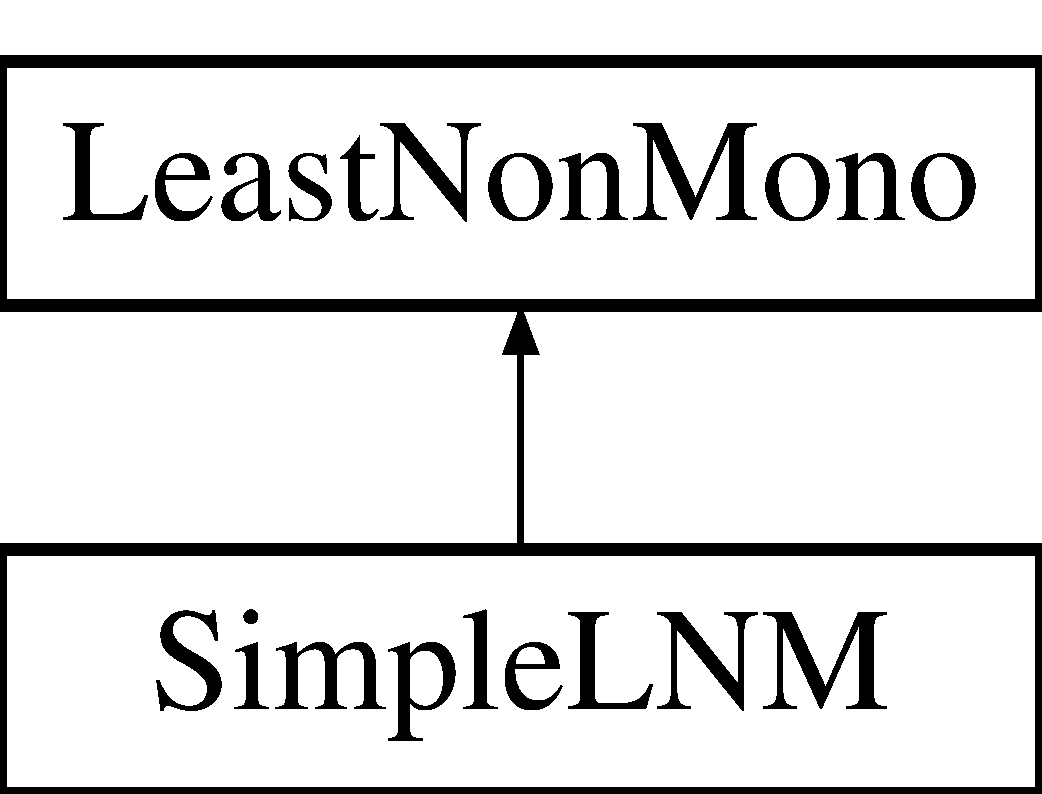
\includegraphics[height=2cm]{d8/dfe/classSimpleLNM}
\end{center}
\end{figure}
\subsection*{Public Member Functions}
\begin{DoxyCompactItemize}
\item 
\hyperlink{classSimpleLNM_a45bd676f6bb504baf1b46ddcbf2f8fb8}{SimpleLNM} (const \hyperlink{classMatrix}{Matrix} \&progVar)
\begin{DoxyCompactList}\small\item\em Constructor. \item\end{DoxyCompactList}\item 
\hypertarget{classSimpleLNM_a89cbe5270c4846ebba8ab1660149112f}{
\hyperlink{classSimpleLNM_a89cbe5270c4846ebba8ab1660149112f}{$\sim$SimpleLNM} ()}
\label{d8/dfe/classSimpleLNM_a89cbe5270c4846ebba8ab1660149112f}

\begin{DoxyCompactList}\small\item\em Destructor. \item\end{DoxyCompactList}\item 
int \hyperlink{classSimpleLNM_a9d296839ca84467c0f6241b1393bd6d5}{LeastNonMonotonic} (int $\ast$monoAry, const int ncols, const int col)
\begin{DoxyCompactList}\small\item\em Method to find the least non monotonic progress variable. \item\end{DoxyCompactList}\end{DoxyCompactItemize}


\subsection{Constructor \& Destructor Documentation}
\hypertarget{classSimpleLNM_a45bd676f6bb504baf1b46ddcbf2f8fb8}{
\index{SimpleLNM@{SimpleLNM}!SimpleLNM@{SimpleLNM}}
\index{SimpleLNM@{SimpleLNM}!SimpleLNM@{SimpleLNM}}
\subsubsection[{SimpleLNM}]{\setlength{\rightskip}{0pt plus 5cm}SimpleLNM::SimpleLNM (const {\bf Matrix} \& {\em progVar})}}
\label{d8/dfe/classSimpleLNM_a45bd676f6bb504baf1b46ddcbf2f8fb8}


Constructor. 

\hyperlink{classSimpleLNM}{SimpleLNM} is a class that determines the least non-\/monotonic progress variable with respect to temperature (or another specified column). It determines the percentage which the progress variable is strictly increasing and the percentage which the progress variable is strictly decreasing. The larger percentage not only determines whether the progress variable is increasing or decreasing, but will also be compared with the percentages of other progress variables. The progress variable with the largest percentage of increasing or decreasing values is the least non-\/monotonic progress variable.

If two or more progress variables share the highest percentage, then the progress variable with the greatest magnitude slope (by endpoints) is selected. Progress variables with neither increasing nor decreasing data are considered strongly non-\/monotonic. 

\subsection{Member Function Documentation}
\hypertarget{classSimpleLNM_a9d296839ca84467c0f6241b1393bd6d5}{
\index{SimpleLNM@{SimpleLNM}!LeastNonMonotonic@{LeastNonMonotonic}}
\index{LeastNonMonotonic@{LeastNonMonotonic}!SimpleLNM@{SimpleLNM}}
\subsubsection[{LeastNonMonotonic}]{\setlength{\rightskip}{0pt plus 5cm}int SimpleLNM::LeastNonMonotonic (int $\ast$ {\em monoAry}, \/  const int {\em ncols}, \/  const int {\em col})\hspace{0.3cm}{\ttfamily  \mbox{[}virtual\mbox{]}}}}
\label{d8/dfe/classSimpleLNM_a9d296839ca84467c0f6241b1393bd6d5}


Method to find the least non monotonic progress variable. 

LeastNonMonotonic calculates how much each progress variable is strictly increasing and strictly decreasing. The input array monoAry will initially be filled with 0s since all progress variables are non-\/monotonic. This method will select the least non-\/monotonic and change its value in monoAry to 1. col is the reference column.

\begin{DoxyVerb}
INPUTS: 

int *monoAry      array containing integer flags that denote the monotonicity of candidate slope variables

const int ncols   number of columns of monoAry

const int col     the reference column

OUTPUT:

int               flag specifying whether or not the function succeeded 
                   = 0: success
		  != 0: something went wrong

\end{DoxyVerb}
 

Implements \hyperlink{classLeastNonMono_a239cbd7836950dc7c758138c4db00d0c}{LeastNonMono}.



The documentation for this class was generated from the following files:\begin{DoxyCompactItemize}
\item 
src/simplelnm.h\item 
src/simplelnm.cc\end{DoxyCompactItemize}

\hypertarget{classleastnonmono_1_1SimpleLNM}{
\section{leastnonmono::SimpleLNM Class Reference}
\label{d8/df0/classleastnonmono_1_1SimpleLNM}\index{leastnonmono::SimpleLNM@{leastnonmono::SimpleLNM}}
}
Inheritance diagram for leastnonmono::SimpleLNM:\begin{figure}[H]
\begin{center}
\leavevmode
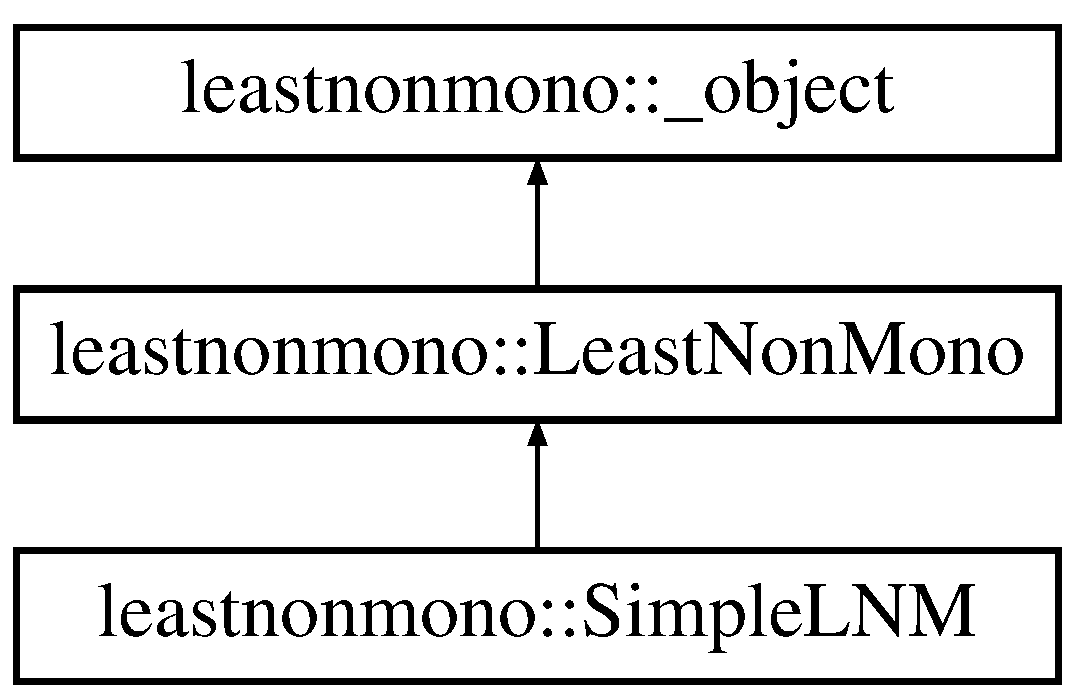
\includegraphics[height=3cm]{d8/df0/classleastnonmono_1_1SimpleLNM}
\end{center}
\end{figure}
\subsection*{Public Member Functions}
\begin{DoxyCompactItemize}
\item 
\hypertarget{classleastnonmono_1_1SimpleLNM_a60b4300be3d34df4505fa4a58eb214dd}{
def {\bfseries \_\-\_\-init\_\-\_\-}}
\label{d8/df0/classleastnonmono_1_1SimpleLNM_a60b4300be3d34df4505fa4a58eb214dd}

\item 
\hypertarget{classleastnonmono_1_1SimpleLNM_ac5c0bed3e296b52b508ad9f45860ac75}{
def {\bfseries LeastNonMonotonic}}
\label{d8/df0/classleastnonmono_1_1SimpleLNM_ac5c0bed3e296b52b508ad9f45860ac75}

\end{DoxyCompactItemize}
\subsection*{Public Attributes}
\begin{DoxyCompactItemize}
\item 
\hypertarget{classleastnonmono_1_1SimpleLNM_a0e7014df02df6a20c4a5d1a78e574303}{
{\bfseries this}}
\label{d8/df0/classleastnonmono_1_1SimpleLNM_a0e7014df02df6a20c4a5d1a78e574303}

\end{DoxyCompactItemize}


The documentation for this class was generated from the following file:\begin{DoxyCompactItemize}
\item 
src/leastnonmono.py\end{DoxyCompactItemize}

\hypertarget{classSimpson}{
\section{Simpson Class Reference}
\label{d7/d99/classSimpson}\index{Simpson@{Simpson}}
}


Calculates integral using Simpson's rule.  




{\ttfamily \#include $<$simpson.h$>$}

Inheritance diagram for Simpson:\begin{figure}[H]
\begin{center}
\leavevmode
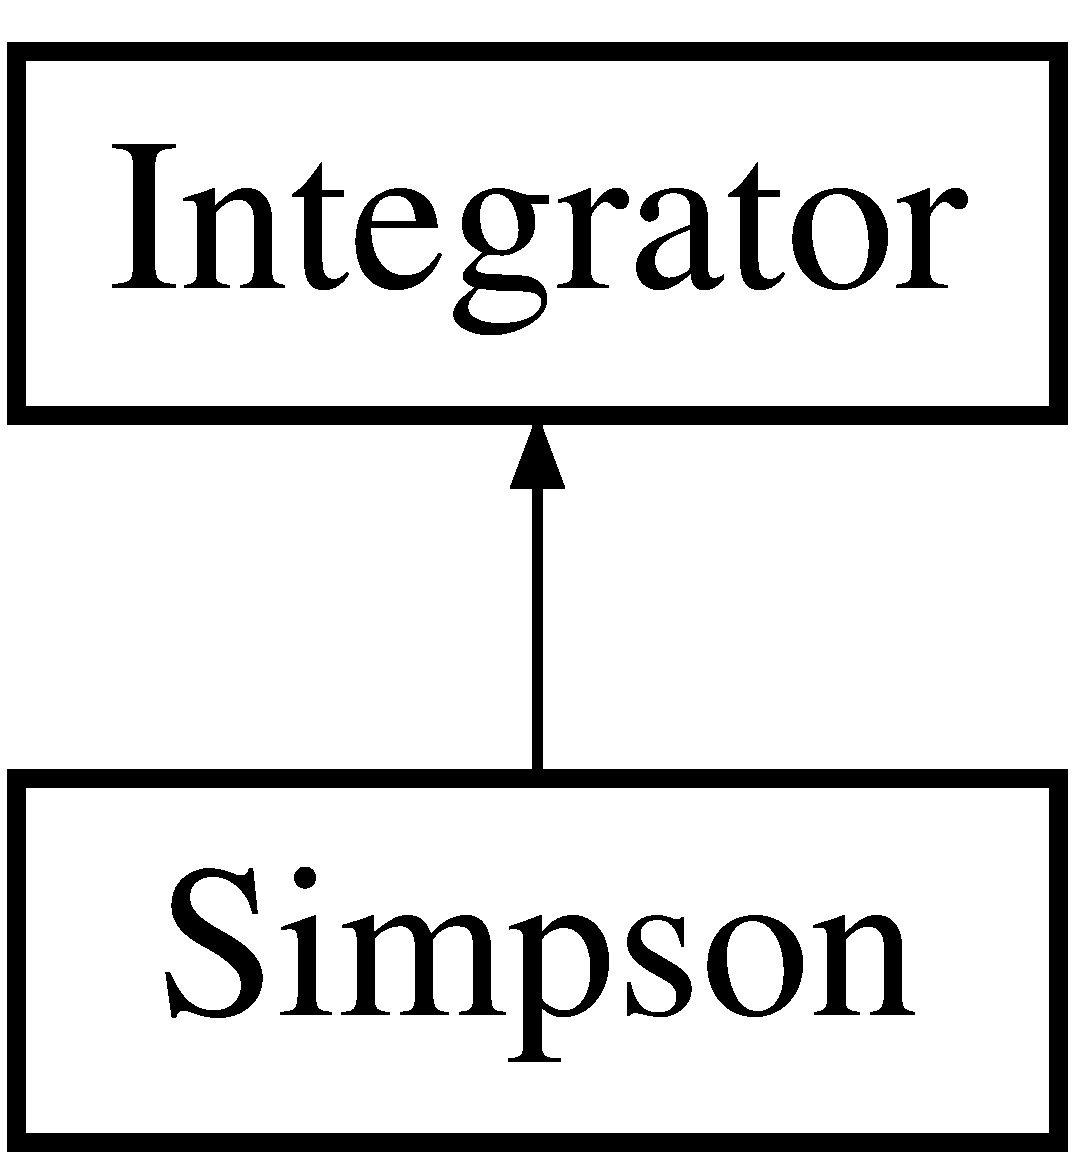
\includegraphics[height=2cm]{d7/d99/classSimpson}
\end{center}
\end{figure}
\subsection*{Public Member Functions}
\begin{DoxyCompactItemize}
\item 
\hypertarget{classSimpson_a67630263e3dafdfaa033f566324b4799}{
\hyperlink{classSimpson_a67630263e3dafdfaa033f566324b4799}{Simpson} ()}
\label{d7/d99/classSimpson_a67630263e3dafdfaa033f566324b4799}

\begin{DoxyCompactList}\small\item\em Constructor. \item\end{DoxyCompactList}\item 
\hypertarget{classSimpson_a92c73e59a11fdf7a156b3682676de6b8}{
\hyperlink{classSimpson_a92c73e59a11fdf7a156b3682676de6b8}{$\sim$Simpson} ()}
\label{d7/d99/classSimpson_a92c73e59a11fdf7a156b3682676de6b8}

\begin{DoxyCompactList}\small\item\em Destructor. \item\end{DoxyCompactList}\item 
double \hyperlink{classSimpson_ab90da2fb197efe2f4a669bf5029a16f4}{integrate} (const double $\ast$integrand, const double $\ast$Z, const int ZPoints)
\begin{DoxyCompactList}\small\item\em Main function that integrates a given data set using Simpson's Rule. \item\end{DoxyCompactList}\end{DoxyCompactItemize}


\subsection{Detailed Description}
Calculates integral using Simpson's rule. \hyperlink{classSimpson}{Simpson} takes in an array (the integrand) and returns the integral of that array using Simpson's rule. 

\subsection{Member Function Documentation}
\hypertarget{classSimpson_ab90da2fb197efe2f4a669bf5029a16f4}{
\index{Simpson@{Simpson}!integrate@{integrate}}
\index{integrate@{integrate}!Simpson@{Simpson}}
\subsubsection[{integrate}]{\setlength{\rightskip}{0pt plus 5cm}double Simpson::integrate (const double $\ast$ {\em integrand}, \/  const double $\ast$ {\em Z}, \/  const int {\em ZPoints})\hspace{0.3cm}{\ttfamily  \mbox{[}virtual\mbox{]}}}}
\label{d7/d99/classSimpson_ab90da2fb197efe2f4a669bf5029a16f4}


Main function that integrates a given data set using Simpson's Rule. 

Simpson's rule is applied to integrate a given integrand over a given double array, Z.

\begin{DoxyVerb}
  INPUTS: 

  const double *integrand           array that contains function values to be integrated

  const double *Z                   array that contains the mixture fraction values which the integrand will be integrated over

  const int ZPoints                 number of values, size of the integrand and Z arrays


  OUTPUT:

  double                            result of the integration

  \end{DoxyVerb}
 

Implements \hyperlink{classIntegrator_a89fbef2f7923ce4e2c979b2ff1d1f4ac}{Integrator}.



The documentation for this class was generated from the following files:\begin{DoxyCompactItemize}
\item 
src/simpson.h\item 
src/simpson.cc\end{DoxyCompactItemize}

\hypertarget{classintegrator_1_1Simpson}{
\section{integrator::Simpson Class Reference}
\label{d0/d4a/classintegrator_1_1Simpson}\index{integrator::Simpson@{integrator::Simpson}}
}
Inheritance diagram for integrator::Simpson:\begin{figure}[H]
\begin{center}
\leavevmode
\includegraphics[height=3cm]{d0/d4a/classintegrator_1_1Simpson}
\end{center}
\end{figure}
\subsection*{Public Member Functions}
\begin{DoxyCompactItemize}
\item 
\hypertarget{classintegrator_1_1Simpson_a17d1008804885fc6afe3790365ffa9e7}{
def {\bfseries \_\-\_\-init\_\-\_\-}}
\label{d0/d4a/classintegrator_1_1Simpson_a17d1008804885fc6afe3790365ffa9e7}

\item 
\hypertarget{classintegrator_1_1Simpson_a8af6b307046196ddefc88456f2341b16}{
def {\bfseries integrate}}
\label{d0/d4a/classintegrator_1_1Simpson_a8af6b307046196ddefc88456f2341b16}

\end{DoxyCompactItemize}
\subsection*{Public Attributes}
\begin{DoxyCompactItemize}
\item 
\hypertarget{classintegrator_1_1Simpson_a891a4cebf60a703f96f1bbd8d1add1e2}{
{\bfseries this}}
\label{d0/d4a/classintegrator_1_1Simpson_a891a4cebf60a703f96f1bbd8d1add1e2}

\end{DoxyCompactItemize}


The documentation for this class was generated from the following file:\begin{DoxyCompactItemize}
\item 
src/integrator.py\end{DoxyCompactItemize}

\hypertarget{classSorting}{
\section{Sorting Class Reference}
\label{da/d2c/classSorting}\index{Sorting@{Sorting}}
}
Inheritance diagram for Sorting:\begin{figure}[H]
\begin{center}
\leavevmode
\includegraphics[height=2cm]{da/d2c/classSorting}
\end{center}
\end{figure}
\subsection*{Public Member Functions}
\begin{DoxyCompactItemize}
\item 
\hypertarget{classSorting_a6686201265fbb31ba9c2071623742be1}{
virtual int \hyperlink{classSorting_a6686201265fbb31ba9c2071623742be1}{sort\_\-data} ()=0}
\label{da/d2c/classSorting_a6686201265fbb31ba9c2071623742be1}

\begin{DoxyCompactList}\small\item\em Virtual function to be inherited by each sorting algorithm to sort the give data. \item\end{DoxyCompactList}\item 
\hypertarget{classSorting_a835629d0133adcdcbf0c56ec05e67ad4}{
virtual void \hyperlink{classSorting_a835629d0133adcdcbf0c56ec05e67ad4}{SetRefColNum} (int num)}
\label{da/d2c/classSorting_a835629d0133adcdcbf0c56ec05e67ad4}

\begin{DoxyCompactList}\small\item\em Setting the reference column according to which the data will be sorted. \item\end{DoxyCompactList}\end{DoxyCompactItemize}


The documentation for this class was generated from the following file:\begin{DoxyCompactItemize}
\item 
src/sorting.h\end{DoxyCompactItemize}

\hypertarget{classsorting_1_1Sorting}{
\section{sorting::Sorting Class Reference}
\label{db/d89/classsorting_1_1Sorting}\index{sorting::Sorting@{sorting::Sorting}}
}
Inheritance diagram for sorting::Sorting:\begin{figure}[H]
\begin{center}
\leavevmode
\includegraphics[height=3cm]{db/d89/classsorting_1_1Sorting}
\end{center}
\end{figure}
\subsection*{Public Member Functions}
\begin{DoxyCompactItemize}
\item 
\hypertarget{classsorting_1_1Sorting_ae3f7a0a90d9d69fbb89b50ebd19117cc}{
def {\bfseries \_\-\_\-init\_\-\_\-}}
\label{db/d89/classsorting_1_1Sorting_ae3f7a0a90d9d69fbb89b50ebd19117cc}

\item 
\hypertarget{classsorting_1_1Sorting_a3fa59303aa54a66068990af025fff245}{
def {\bfseries sort\_\-data}}
\label{db/d89/classsorting_1_1Sorting_a3fa59303aa54a66068990af025fff245}

\item 
\hypertarget{classsorting_1_1Sorting_a0d3b5cfd6277d7cabaef8b139315ad6d}{
def {\bfseries SetRefColNum}}
\label{db/d89/classsorting_1_1Sorting_a0d3b5cfd6277d7cabaef8b139315ad6d}

\end{DoxyCompactItemize}


The documentation for this class was generated from the following file:\begin{DoxyCompactItemize}
\item 
src/sorting.py\end{DoxyCompactItemize}

\hypertarget{classStandardSort}{
\section{StandardSort Class Reference}
\label{d0/d94/classStandardSort}\index{StandardSort@{StandardSort}}
}
Inheritance diagram for StandardSort:\begin{figure}[H]
\begin{center}
\leavevmode
\includegraphics[height=2cm]{d0/d94/classStandardSort}
\end{center}
\end{figure}
\subsection*{Public Member Functions}
\begin{DoxyCompactItemize}
\item 
\hyperlink{classStandardSort_afecdf65f1388c1d23339c99f799131fd}{StandardSort} (\hyperlink{classMatrix}{Matrix} $\ast$data)
\begin{DoxyCompactList}\small\item\em Constructor. \item\end{DoxyCompactList}\item 
\hypertarget{classStandardSort_a71e4c8dff2b71dcf0958babaf2e3beb8}{
\hyperlink{classStandardSort_a71e4c8dff2b71dcf0958babaf2e3beb8}{$\sim$StandardSort} ()}
\label{d0/d94/classStandardSort_a71e4c8dff2b71dcf0958babaf2e3beb8}

\begin{DoxyCompactList}\small\item\em Destructor. \item\end{DoxyCompactList}\item 
int \hyperlink{classStandardSort_ae0c7e47ba48c319989b41815b0724f41}{sort\_\-data} ()
\begin{DoxyCompactList}\small\item\em Main function that sorts the given data. \item\end{DoxyCompactList}\item 
\hypertarget{classStandardSort_afdf7549b717b75c6274697fddcb75c8a}{
void \hyperlink{classStandardSort_afdf7549b717b75c6274697fddcb75c8a}{SetRefColNum} (int num)}
\label{d0/d94/classStandardSort_afdf7549b717b75c6274697fddcb75c8a}

\begin{DoxyCompactList}\small\item\em Set the reference column number. \item\end{DoxyCompactList}\end{DoxyCompactItemize}


\subsection{Constructor \& Destructor Documentation}
\hypertarget{classStandardSort_afecdf65f1388c1d23339c99f799131fd}{
\index{StandardSort@{StandardSort}!StandardSort@{StandardSort}}
\index{StandardSort@{StandardSort}!StandardSort@{StandardSort}}
\subsubsection[{StandardSort}]{\setlength{\rightskip}{0pt plus 5cm}StandardSort::StandardSort ({\bf Matrix} $\ast$ {\em data})}}
\label{d0/d94/classStandardSort_afecdf65f1388c1d23339c99f799131fd}


Constructor. 

The data to be sorted is passed to the constructor. A duplicate of the data is produced to be later at this stage 

\subsection{Member Function Documentation}
\hypertarget{classStandardSort_ae0c7e47ba48c319989b41815b0724f41}{
\index{StandardSort@{StandardSort}!sort\_\-data@{sort\_\-data}}
\index{sort\_\-data@{sort\_\-data}!StandardSort@{StandardSort}}
\subsubsection[{sort\_\-data}]{\setlength{\rightskip}{0pt plus 5cm}int StandardSort::sort\_\-data ()\hspace{0.3cm}{\ttfamily  \mbox{[}virtual\mbox{]}}}}
\label{d0/d94/classStandardSort_ae0c7e47ba48c319989b41815b0724f41}


Main function that sorts the given data. 

The algorithm sends the reference column to the standard sorting operator that is embedded into the C++ standard library

\begin{DoxyVerb}
  INPUT 

  There are no inputs. The data to be sorted is already passed via the constructor

  OUTPUT:

  int       flag specifying whether or not the function succeeded
             = 0: success
	    != 0: something went wrong

\end{DoxyVerb}
 

Implements \hyperlink{classSorting_a6686201265fbb31ba9c2071623742be1}{Sorting}.



The documentation for this class was generated from the following files:\begin{DoxyCompactItemize}
\item 
src/standardsort.h\item 
src/standardsort.cc\end{DoxyCompactItemize}

\hypertarget{classsorting_1_1StandardSort}{
\section{sorting::StandardSort Class Reference}
\label{d2/d3e/classsorting_1_1StandardSort}\index{sorting::StandardSort@{sorting::StandardSort}}
}
Inheritance diagram for sorting::StandardSort:\begin{figure}[H]
\begin{center}
\leavevmode
\includegraphics[height=3cm]{d2/d3e/classsorting_1_1StandardSort}
\end{center}
\end{figure}
\subsection*{Public Member Functions}
\begin{DoxyCompactItemize}
\item 
\hypertarget{classsorting_1_1StandardSort_a8f565d310ca5114b4df5c8786b5ded14}{
def {\bfseries \_\-\_\-init\_\-\_\-}}
\label{d2/d3e/classsorting_1_1StandardSort_a8f565d310ca5114b4df5c8786b5ded14}

\item 
\hypertarget{classsorting_1_1StandardSort_a7135230313eba673cb6bb4db808a5188}{
def {\bfseries sort\_\-data}}
\label{d2/d3e/classsorting_1_1StandardSort_a7135230313eba673cb6bb4db808a5188}

\item 
\hypertarget{classsorting_1_1StandardSort_aa42465972d6629637a8954d505c2733b}{
def {\bfseries SetRefColNum}}
\label{d2/d3e/classsorting_1_1StandardSort_aa42465972d6629637a8954d505c2733b}

\end{DoxyCompactItemize}
\subsection*{Public Attributes}
\begin{DoxyCompactItemize}
\item 
\hypertarget{classsorting_1_1StandardSort_a55c05fdd3c2de1fec0fe2312feb70d91}{
{\bfseries this}}
\label{d2/d3e/classsorting_1_1StandardSort_a55c05fdd3c2de1fec0fe2312feb70d91}

\end{DoxyCompactItemize}


The documentation for this class was generated from the following file:\begin{DoxyCompactItemize}
\item 
src/sorting.py\end{DoxyCompactItemize}

\hypertarget{classTrapz}{
\section{Trapz Class Reference}
\label{d8/da8/classTrapz}\index{Trapz@{Trapz}}
}


Calculates integral using the trapezoidal method.  




{\ttfamily \#include $<$trapz.h$>$}

Inheritance diagram for Trapz:\begin{figure}[H]
\begin{center}
\leavevmode
\includegraphics[height=2cm]{d8/da8/classTrapz}
\end{center}
\end{figure}
\subsection*{Public Member Functions}
\begin{DoxyCompactItemize}
\item 
\hypertarget{classTrapz_a464cc7e5b33620d799cb89f69f70f1b4}{
\hyperlink{classTrapz_a464cc7e5b33620d799cb89f69f70f1b4}{Trapz} ()}
\label{d8/da8/classTrapz_a464cc7e5b33620d799cb89f69f70f1b4}

\begin{DoxyCompactList}\small\item\em Constructor. \item\end{DoxyCompactList}\item 
\hypertarget{classTrapz_adff2586590ecb48620b749a0966f32a7}{
\hyperlink{classTrapz_adff2586590ecb48620b749a0966f32a7}{$\sim$Trapz} ()}
\label{d8/da8/classTrapz_adff2586590ecb48620b749a0966f32a7}

\begin{DoxyCompactList}\small\item\em Destructor. \item\end{DoxyCompactList}\item 
double \hyperlink{classTrapz_a8aee327ed631f75ef3dea7e458f71cca}{integrate} (const double $\ast$integrand, const double $\ast$Z, const int ZPoints)
\begin{DoxyCompactList}\small\item\em Main function that integrates a given data set using Trapezoidal Rule. \item\end{DoxyCompactList}\end{DoxyCompactItemize}


\subsection{Detailed Description}
Calculates integral using the trapezoidal method. \hyperlink{classTrapz}{Trapz} takes in an array (the integrand) and returns the integral of that array using the trapezoidal method. 

\subsection{Member Function Documentation}
\hypertarget{classTrapz_a8aee327ed631f75ef3dea7e458f71cca}{
\index{Trapz@{Trapz}!integrate@{integrate}}
\index{integrate@{integrate}!Trapz@{Trapz}}
\subsubsection[{integrate}]{\setlength{\rightskip}{0pt plus 5cm}double Trapz::integrate (const double $\ast$ {\em integrand}, \/  const double $\ast$ {\em Z}, \/  const int {\em ZPoints})\hspace{0.3cm}{\ttfamily  \mbox{[}virtual\mbox{]}}}}
\label{d8/da8/classTrapz_a8aee327ed631f75ef3dea7e458f71cca}


Main function that integrates a given data set using Trapezoidal Rule. 

Trapezoidal rule is applied to integrate a given integrand over a given double array, Z.

\begin{DoxyVerb}
  INPUTS:

  const double *integrand          array that contains function values to be integrated

  const double *Z                  array that contains the mixture fraction values which the integrand will be integrated over

  const int ZPoints                number of values, size of the integrand and Z containers

  
  OUTPUT:

  double                           result of the integration
 
  \end{DoxyVerb}
 

Implements \hyperlink{classIntegrator_a89fbef2f7923ce4e2c979b2ff1d1f4ac}{Integrator}.



The documentation for this class was generated from the following files:\begin{DoxyCompactItemize}
\item 
src/trapz.h\item 
src/trapz.cc\end{DoxyCompactItemize}

\hypertarget{classintegrator_1_1Trapz}{
\section{integrator::Trapz Class Reference}
\label{db/dc8/classintegrator_1_1Trapz}\index{integrator::Trapz@{integrator::Trapz}}
}
Inheritance diagram for integrator::Trapz:\begin{figure}[H]
\begin{center}
\leavevmode
\includegraphics[height=3cm]{db/dc8/classintegrator_1_1Trapz}
\end{center}
\end{figure}
\subsection*{Public Member Functions}
\begin{DoxyCompactItemize}
\item 
\hypertarget{classintegrator_1_1Trapz_a20001d1505a9f9f5d6412e707c99a28c}{
def {\bfseries \_\-\_\-init\_\-\_\-}}
\label{db/dc8/classintegrator_1_1Trapz_a20001d1505a9f9f5d6412e707c99a28c}

\item 
\hypertarget{classintegrator_1_1Trapz_af8fade81b71ebd43ea4d8c93b7dbc490}{
def {\bfseries integrate}}
\label{db/dc8/classintegrator_1_1Trapz_af8fade81b71ebd43ea4d8c93b7dbc490}

\end{DoxyCompactItemize}
\subsection*{Public Attributes}
\begin{DoxyCompactItemize}
\item 
\hypertarget{classintegrator_1_1Trapz_a591c3fae4b831990a14bf6ac6203d599}{
{\bfseries this}}
\label{db/dc8/classintegrator_1_1Trapz_a591c3fae4b831990a14bf6ac6203d599}

\end{DoxyCompactItemize}


The documentation for this class was generated from the following file:\begin{DoxyCompactItemize}
\item 
src/integrator.py\end{DoxyCompactItemize}

\chapter{File Documentation}
\hypertarget{convolute_8cc}{
\section{src/convolute.cc File Reference}
\label{d4/db1/convolute_8cc}\index{src/convolute.cc@{src/convolute.cc}}
}
{\ttfamily \#include \char`\"{}convolute.h\char`\"{}}\par
{\ttfamily \#include \char`\"{}matrix.h\char`\"{}}\par
{\ttfamily \#include \char`\"{}matrix3d.h\char`\"{}}\par
{\ttfamily \#include \char`\"{}math.h\char`\"{}}\par
\subsection*{Functions}
\begin{DoxyCompactItemize}
\item 
int \hyperlink{convolute_8cc_a4dc63393d8024c8d83caa68eed073629}{convVal} (double $\ast$Z, double $\ast$data, \hyperlink{classMatrix3D}{Matrix3D} $\ast$pdfValues, \hyperlink{classMatrix}{Matrix} $\ast$postConvVal, \hyperlink{classIntegrator}{Integrator} $\ast$intgr)
\begin{DoxyCompactList}\small\item\em Convolution function. \item\end{DoxyCompactList}\end{DoxyCompactItemize}


\subsection{Detailed Description}


\subsection{Function Documentation}
\hypertarget{convolute_8cc_a4dc63393d8024c8d83caa68eed073629}{
\index{convolute.cc@{convolute.cc}!convVal@{convVal}}
\index{convVal@{convVal}!convolute.cc@{convolute.cc}}
\subsubsection[{convVal}]{\setlength{\rightskip}{0pt plus 5cm}int convVal (double $\ast$ {\em Z}, \/  double $\ast$ {\em data}, \/  {\bf Matrix3D} $\ast$ {\em pdfValues}, \/  {\bf Matrix} $\ast$ {\em postConvVal}, \/  {\bf Integrator} $\ast$ {\em intgr})}}
\label{d4/db1/convolute_8cc_a4dc63393d8024c8d83caa68eed073629}


Convolution function. 

Convolutes date and pdf. 
\hypertarget{fittogrid_8cc}{
\section{src/fittogrid.cc File Reference}
\label{d0/dc2/fittogrid_8cc}\index{src/fittogrid.cc@{src/fittogrid.cc}}
}
{\ttfamily \#include \char`\"{}fittogrid.h\char`\"{}}\par
{\ttfamily \#include \char`\"{}matrix.h\char`\"{}}\par
{\ttfamily \#include \char`\"{}matrix3d.h\char`\"{}}\par
{\ttfamily \#include \char`\"{}interpolator.h\char`\"{}}\par
{\ttfamily \#include $<$iostream$>$}\par
{\ttfamily \#include $<$algorithm$>$}\par
{\ttfamily \#include $<$vector$>$}\par
{\ttfamily \#include \char`\"{}sorting.h\char`\"{}}\par
{\ttfamily \#include $<$omp.h$>$}\par
\subsection*{Functions}
\begin{DoxyCompactItemize}
\item 
int \hyperlink{fittogrid_8cc_abc7a89647a0f024f3c265c7b4f390b7f}{fittogrid} (const \hyperlink{classMatrix4D}{Matrix4D} $\ast$datain, const double $\ast$cgrid, \hyperlink{classInterpolator}{Interpolator} $\ast$interp, \hyperlink{classMatrix3D}{Matrix3D} $\ast$dataout, int nthreads, int ex)
\begin{DoxyCompactList}\small\item\em Function which fits data to a grid. \item\end{DoxyCompactList}\end{DoxyCompactItemize}


\subsection{Detailed Description}


\subsection{Function Documentation}
\hypertarget{fittogrid_8cc_abc7a89647a0f024f3c265c7b4f390b7f}{
\index{fittogrid.cc@{fittogrid.cc}!fittogrid@{fittogrid}}
\index{fittogrid@{fittogrid}!fittogrid.cc@{fittogrid.cc}}
\subsubsection[{fittogrid}]{\setlength{\rightskip}{0pt plus 5cm}int fittogrid (const {\bf Matrix4D} $\ast$ {\em datain}, \/  const double $\ast$ {\em cgrid}, \/  {\bf Interpolator} $\ast$ {\em interp}, \/  {\bf Matrix3D} $\ast$ {\em dataout}, \/  int {\em nthreads}, \/  int {\em ex})}}
\label{d0/dc2/fittogrid_8cc_abc7a89647a0f024f3c265c7b4f390b7f}


Function which fits data to a grid. 

This function takes in a 4D matrix and fits the data onto a specified grid.

\begin{DoxyVerb}
  INPUTS:

  Matrix4D *datain       input data stored as a 4D matrix. The structure is (mean, z~, z_v, file), where
                         mean has dimension 2 and contains w~ and c~. datain can be thought of as two 3D
                         matrices with structure (z~, z_v, file) containing values of w~ and c~, 
                         respectively. 

  const double *cgrid    pointer to an array which contains the values of c~ at which to interpolate

  Interpolator *interp   pointer to an Interpolator object

  Matrix3D *dataout      output data stored as a 3D matrix. The structure is (z~, z_v, cgrid), with the 
                         numbers being interpolated values of w~

  int numthreads         integer specifying the number of threads to be used (1 = serial, >1 = parallel)

  int ex                 integer specifying whether or not to extrapolate (0 = no, 1 = yes)


  OUTPUTS:

  int                    flag specifying whether or not extrapolation was necessary:
                         = 0: no extrapolation
			 = 1: extrapolation performed
\end{DoxyVerb}
 
\printindex
\end{document}
